\documentclass[a4paper, 12pt, openright, oneside, german, french, english, brazil]{abntex2}
\usepackage[brazil]{babel}
\usepackage{graphicx}
\usepackage[utf8]{inputenc}
\usepackage{wrapfig}
\usepackage{lscape}
\usepackage{rotating}
\usepackage{epstopdf}
\usepackage[alf]{abntex2cite}
\usepackage[a4paper, left=3cm, right=2cm, top=3cm, bottom=2cm]{geometry}
\usepackage{indentfirst}
\usepackage{longtable}
\usepackage{amsmath}
\usepackage{verbatim}
\usepackage{algorithm}
\floatname{algorithm}{Código}
\renewcommand{\listalgorithmname}{Lista de Códigos}
\usepackage{algpseudocode} %para escrever pseudo-algoritmos
%\algrenewcommand\algorithmicwhile{\textbf{Enquanto}}
%\algrenewcommand\algorithmicfor{\textbf{Para}}
%\algrenewcommand\algorithmicif{\textbf{Se}}
%\algrenewcommand\algorithmicthen{\textbf{então}}
%\algrenewcommand\algorithmicelse{\textbf{Do contrário}}
%\algrenewcommand\algorithmicdo{\textbf{faça}}
%\algrenewcommand\algorithmicfunction{\textbf{Função}}
%\algrenewcommand\algorithmicend{\textbf{termina}}
\usepackage{listings} %para escrever códigos
\pagestyle{plain}

\titulo{\textbf{A Construção Social da Qualidade no Mercado da Música de Concerto}}
\autor{Neylson J. B. F. Crepalde}
\data{Agosto, 2017}
\instituicao{UNIVERSIDADE FEDERAL DE MINAS GERAIS
	\par
	Faculdade de Filososia e Ciências Humanas}
\local{Belo Horizonte}
\orientador{Dr. Silvio Salej Higgins}
\preambulo{Projeto de tese apresentado ao programa de pós-graduação em sociologia como requisito parcial à obtenção do título de Doutor em Sociologia.

	Linha de Pesquisa: Sociologia Econômica e das Organizações}
\tipotrabalho{Tese (doutorado)}


\begin{document}
	\pretextual
	%\imprimircapa
	\imprimirfolhaderosto

	%	\begin{dedicatoria}
	%		\vspace*{\fill}
	%		Dedico este trabalho a \ldots
	%		\vspace*{\fill}
	%	\end{dedicatoria}

	%\begin{agradecimentos}
	%	Gostaria de agradecer \ldots
	%\end{agradecimentos}

	%\begin{epigrafe}
	%	\vspace*{\fill}
	%	\begin{flushright}
	%		\textit{Não é da benevolência do violinista, do maestro e do diretor artístico que esperamos a nossa \textbf{música}, mas da consideração que ele tem pelos prórprios interesses.\\
	%			(parafraseando Adam Smith)}
	%	\end{flushright}
	%\end{epigrafe}

	%% --- resumo em português ---
	%\begin{resumo}
	%	Resumo em português\\
	%	\vspace{\onelineskip}
	%	\noindent
	%	\textbf{Palavras-chave}: latex. abntex. editoração de texto.
	%\end{resumo}
	%% --- resumo em inglês ---
	%\begin{resumo}[Abstract]
	%	\begin{otherlanguage*}{english}
	%		The abstract in english.\\
	%		\vspace{\onelineskip}
	%		\noindent
	%		\textbf{Keywords}: latex. abntex. publication of texts.
	%	\end{otherlanguage*}
	%\end{resumo}
	%% --- resumo em francês ---
	%\begin{resumo}[Résumé]
	%	\begin{otherlanguage*}{french}
	%		Il s’agit d’un résumé en français.\\
	%		\vspace{\onelineskip}
	%		\noindent
	%		\textbf{Mots-clés}: latex. abntex. publication de textes.
	%	\end{otherlanguage*}
	%\end{resumo}

%	\listofalgorithms
	\listoffigures
	\listoftables
	\newpage
	\tableofcontents
	\textual

	\chapter*[Introdução]{Introdução}
	\addcontentsline{toc}{chapter}{INTRODUÇÃO}

	Para que o produto final por excelência de uma orquestra, a saber o concerto, venha a existir e chegue ao seu destino, o público, uma série de atores se envolvem em diversos processos de cooperação e mobilizam uma série de recursos construindo um sistema de produção em rede, ou o que Howard Becker chamaria de um ``mundo da arte'' (\textit{Art World}). Para \citeonline[p. 1, tradução do autor]{becker2008art}, ``a existência de mundos da arte, bem como o modo como sua existência afeta tanto a produção quanto o consumo de obras de arte, sugere uma abordagem sociológica para as artes'' \footnote{The existence of art worlds, as well as the way their existence affects both the production and consumption of art works, suggests a sociological approach to the arts.}.


	%\begin{citacao}
	%	Os mundos da arte consistem de todas as pessoas cujas atividades são necessárias para a produção de obras características que aquele mundo, e talvez outros ainda, definem como arte. Membros dos mundos da arte coordenam as atividades pelas quais a obra é produzida referindo-se a um corpo de entendimentos convencionais incorporados na prática comum e nos artefatos comumente usados. As mesmas pessoas frequentemente cooperam repetidamente, até mesmo rotineiramente, de formas similares para produzir obras similares, portanto podemos pensar em um mundo da arte como uma rede de conexões de cooperação entre os participantes estabelecida.\footnote{Art worlds consist of all the people whose activities are necessary to the production of the characteristic works which that world, and perhaps others as well, define as art. Members of art worlds coordinate the activities by which work is produced by referring to a body of conventional understandings embodied in common practice and in frequently used artifacts. The same people often cooperate repeatedly, in similar ways to produce similar works, so that we can think of an art world as an established network of cooperative links among participants.} \cite[p. 34-5]{becker2008art}

	%\end{citacao}



	%Para que os concertos aconteçam, a orquestra (formada pelos instrumentistas, pelo maestro, pela administração e ainda pela instituição mantenedora) toca uma obra escrita por um compositor em uma notação convencionada. Os instrumentistas tocam em instrumentos construídos por um luthier de uma maneira também convencionada. Para que o concerto aconteça, é preciso que exista uma demanda por ele. Por isso, além da orquestra, participam do evento o público consumidor do espetáculo, os meios de divulgação pelos quais esse público toma conhecimento do concerto, o Estado como regulador e financiador, as empresas privadas que também financiam a orquestra, além de diversos outros atores com papeis menores, embora igualmente importantes (iluminadores, técnicos de som, funcionários da bilheteria, copistas, arquivistas, montadores, etc.).


	Por outro lado, se prestamos atenção à dinâmica comum aos mercados, o que percebemos com maior facilidade é um ambiente altamente concorrencial. O fenômeno supracitado é abordado por \citeonline{lazega2009theorie} de uma perspectiva distinta: no mundo concorrencial, os atores se veem constantemente em situações em que buscam a estabilidade do mercado tornando-o viável. Isso não acontece simplesmente de acordo com a lei da oferta e da demanda mas a partir do posicionamento dos produtores numa escala de qualidade que diferencia seus produtos. Para que isso seja possível, a concorrência total é inviável já que existe uma parcela de interdependência entre produtores. Essa visão está ancorada na perspectiva relacional a qual concebe mercados como estruturas sociais, empresas, Estados, etc., como estruturas em rede \cite{white2008,white2002markets,lazega2014redes}.


	O foco deste trabalho é descortinar o mercado da música de concerto. Esse mercado ainda permanece fora do interesse convencional de economistas, sociólogos e demais estudiosos dos mercados, talvez por uma mera obra do acaso, talvez por sua alta complexidade e especificidade. Antes de apresentar nossas perguntas de pesquisa e nossos objetivos, faz-se necessário uma imersão na literatura de base realizando uma revisão tão profunda quanto possível. Após essa revisão, tentaremos extrair da observação da própria literatura (considerando o que já está postulado e, sobretudo, as lacunas existentes) os rumos de nossa investigação.

	Desse modo, iniciaremos o trabalho apresentando brevemente o marco teórico do qual partimos para compreender nosso objeto de pesquisa, a sociologia neoestrutural. Em seguida, apresentaremos uma pesquisa bibliográfica realizada em duas das principais bases de produção acadêmica disponíveis na área de sociologia e economia. Encontramos que a produção científica sobre o mercado da música de concerto nos últimos 30 anos é ínfima. Depois, investigaremos na teoria econômica o conhecimento já sedimentado sobre bens culturais buscando entender os desafios colocados por nosso objeto de pesquisa. No terceiro capítulo, apresentaremos o framework teórico adotado para as análises, qual seja, a Análise de Redes Sociais (\textit{Social Network Analysis})\footnote{Muito embora, antecipamos, as ferramentas conhecidas como \textit{social network analysis} não constituem uma teoria geral do mundo que dedutivamente se aplique a qualquer realidade complexa. Trata-se, aqui, de um conjunto de ferramentas metodológicas aliadas a uma concepção de relações sociais.}. No quarto capítulo apresentaremos o desenho de pesquisa explicitando que tipo de dados intencionamos coletar, os procedimentos adotados, as formas de análises e os resultados esperados. Por fim, apresentamos uma investigação preliminar iniciada com uma das orquestras da cidade de Belo Horizonte bem como as considerações finais deste projeto.



	%Para o autor, ``a construção coletiva da qualidade implica que a viabilidade do mercado vem do coletivo, e que é a estrutura do conjunto do mercado viável que cria a divisão de lucros\footnote{La construction collective de la qualité implique ainsi que la viabilité du marché vient du collectif, et que c'est la structure d'ensemble du marché viable qui crée le partage des rentes.}'' \cite[p. 563, tradução do autor]{lazega2009theorie}.



	%Desse modo, para que esse mercado viável seja possível, é necessário que que as empresas se engajem constantemente numa combinação estável de concorrência e de cooperação. A emergência de uma estrutura a partir das próprias relações assimétricas entre eles pode criar vantagens para alguns. Para \citeonline{lazega2009theorie}, ``as relações de poder e os controles que eles exercem sobre as negociações são, portanto, cruciais nesse modelo. Sobre esse tipo de mercado, por definição, a troca não é jamais bilaterial, sempre multilateral e estratégica\footnote{Les relations de pouvoir et les contraintes qu'elles font peser sur les négociations sont donc cruciales dans ce modèle. Sur ce type de marché, par définition, l'échange n'est jamais bilatéral, toujours multilatéral et stratégique.}'' \cite[p. 563, tradução do autor]{lazega2009theorie}. Esse fenômeno é conhecido na literatura como \textit{coopetition}. A partir das perspectivas apresentadas, entramos na problemática que conduz nossa investigação.



	%\subsection*{Problemas de Pesquisa}

	%\addcontentsline{toc}{section}{Problema de Pesquisa e Objetivos}





	\begin{comment}

	na região Sudeste do Brasil. A investigação é norteada por duas principais perguntas: 1) Entendendo que o mercado das orquestras não opera como um mercado comum, como se dá seu funcionamento; quem são os atores envolvidos e quais são as ações que cada um desenvolve no sistema? 2)Quais são as condições e fatores sociais de produção de padrões de qualidade da música de concerto, ou seja, como é produzido e mantido o \textit{standard} de qualidade com o qual todos estão comprometidos?



	Para desenvolvermos nosso estudo faz-se necessário transcender os limites com os quais a teoria econômica se deparou ao abordar produtos culturais. Ora, em todo o seu decurso, a teoria econômica tem ancorado seus principais achados em dois pressupostos. O primeiro remonta à ideia do \textit{homo economicus}, ou seja, o ator racional que toma decisões visando potencializar ganhos e diminuir perdas. Para isso, ele tem acesso à completude das informações de que precisa e é capaz de processá-las inteiramente. Esse pressuposto dá à economia a capacidade de elaborar modelos elegantes para explicar escolhas e preferências mas não consegue incorporar uma parte central da vida social, a saber, a cultura. A área da sociologia econômica desenvolveu-se, sobretudo, se debruçando sobre as lacunas deixadas por esse pressuposto buscando dar conta de como normas sociais, valores, sistemas de status e prestígio influenciam a ação econômica. Dito de outra forma, uma perspectiva sociológica possibilita enxergar fatores relacionais que ajudam a responder a perguntas clássicas da economia além de tornar o estudo mais próximo da realidade mesmo não tendo modelos tão elegantes e nem lógica tão consistente \cite{hirsch1987dirty}. A sociologia econômica está preocupada com elementos contextuais das trocas econômicas, ou seja, analisar como as interações entre os atores fazem emergir um mercado e como essas interações regulam e controlam os mercados.











	O segundo pressuposto consiste da caracterização geral dos produtos mercantis. Nessa caracterização, as mercadorias são entendidas por meio de quatro critérios objetivos, a saber, suas propriedades físicas (as quais, nesse caso, estão diretamente relacionadas com a qualidade do produto em questão), a data e o local em que estão disponíveis e aquilo que condiciona sua entrega num universo certo, i.e., sem incertezas. A qualidade de um bem, nessa perspectiva, pode ser decomposta em uma série de elementos objetivos, i.e., claramente mensuráveis e hierarquizáveis. Além disso, na teoria econômica clássica todo bem é considerado um ``bem privado'' e, portanto, ``exclusivo e rival'' no consumo. Para citar um exemplo, ``um café, um sanduíche, uma camisa, um par de sapatos, uma cadeira, etc., são bens exclusivos porque é possível impedir-me de obtê-los (\ldots); por outro lado, cada um desses bens é de consumo exclusivo porque no momento em que o aproveito, nenhuma outra pessoa pode usufruí-lo'' \cite[p. 29]{tolila2007cultura}. Ora, os produtos culturais, de um modo geral, são não exclusivos; pode-se, por exemplo, admirar um belo edifício histórico na rua sem ter que pagar por isso. Tampouco são rivais no consumo; o prazer de assistir um concerto não é diminuído pela presença de outras pessoas no público.



	O setor cultural define-se, ainda, pela sua lógica de oferta voltada à produção, ao contrário dos mercados de bens comuns voltados ao consumo. Para \citeonline[p. 32]{tolila2007cultura}, ``essa lógica da oferta caracteriza bem, entre outras, a ação das políticas públicas em termos de investimento, de ajuda e de sustentação das atividades culturais, do patrimônio ao espetáculo ao vivo, e em termos de incentivos às práticas culturais''. De fato, os Estados e coletividades públicas tem demonstrado interesse crescente no setor cultural, o que pode ser verificado através das políticas públicas, das administrações especializadas, da alocação de recursos dirigidos especificamente ao setor e do surgimento de toda uma rede de instituições e profissionais atuantes no setor cultural, grande parte deles financiados por dinheiro público \cite{tolila2007cultura}.



	O valor simbólico dos bens culturais constitui, para nós, um elemento central na compreensão de nosso objeto de estudo, muito embora, contrariando novamente a teoria econômica clássica, não seja objetivo em sua natureza mas relacional e individual, i.e., só existe à medida que é reconhecido pelo indivíduo no momento de seu consumo. Para que o valor simbólico de um determinado bem seja reconhecido, é necessário que haja estruturas cognitivas apropriadas para a compreensão e fruição do bem, ou seja, esquemas mentais adquiridos por meio da educação artística prévia \cite{bourdieu2003amor}.



	As performances musicais possuem ainda uma particularidade quanto à natureza de sua existência na qual reside grande parte das dificuldades metodológicas que as cercam. \citeonline{tolila2007cultura} explica:



	\begin{citacao}

		O que é a música? A partitura escrita? Não. Os músicos que formam a orquestra? Não. O regente? Também não. Na verdade, é quase impossível definir a música como uma ``coisa'' (uma mesa, uma cadeira, uma casa, etc.) pois ela só existe de fato no momento em que é ouvida, isto é, em uma relação com o ouvinte\footnote{Para o autor, ``na verdade, no mundo social, o modo real de existência da maioria dos fenômenos é o da relação entre seres humanos'' \cite[p. 110]{tolila2007cultura}. Curiosamente, nessa premissa se baseia todo o paradigma neoestrutural na sociologia conhecido também como ``perspectiva relacional'' ou ``teoria das redes sociais''.}. \cite[p. 109]{tolila2007cultura}

	\end{citacao}



	Desse modo, a música (bem como a dança e o teatro, por exemplo) assume um modo especial de existência que envolve a participação de todos os elementos ou atores supracitados, a saber, partitura, músicos, regente, etc., na construção de sua materialidade que só existe (e portanto só é possível de ser consumida) no momento da escuta.



	\citeonline{karpik2009elements} trata o mesmo objeto sob a ótica da ``economia de singularidades''. Para esse autor, bens e serviços singulares ``são desconhecidos pela teoria econômica neoclássica. Eles não existem''\footnote{(\dots) ils sont donc méconnus par la théorie économique néo-classique. Ils n'existent pas.} \cite[p. 163]{karpik2009elements}. As singularidades são sinalizadas pela presença do \textit{bom} em sua caracterização como diferencial numa comparação entre qualidades, i.e., o bom vinho, a boa música, a boa orquestra, etc.



	\begin{citacao}

		As singularidades são bens e serviços \textit{estruturados, incertos e incomensuráveis}. Essas três características \textit{combinadas} caracterizam todas as singularidades como sendo únicas, múltiplas e seu suporte material prescinde da produção industrial, uma vez que seja mantido o seu poder simbólico e, por conseguinte, sua capacidade de acolher um número indeterminado de interpretações particulares\footnote{Les singularités sont des biens et services \textit{structurés, incertains et incommensurables.} Ces trois traits \textit{combinés} caractérisent toutes les singularités que'elles soient uniques, multiples ou que leurs supports matériels relèvent de la production industrielle, dès lors qu'est maintenu leur pouvoir symbolique et, par voie de conséquence, leur capacité à accueillir un nombre indéterminé d'interprétations particulières.}. \cite[p. 164]{karpik2009elements}

	\end{citacao}



	\end{comment}









	% Segundo \citeonline[p. 54]{benhamou2007economia} ``a concorrência assume a forma paradoxal de uma competição entre instituições que oferecem bens únicos e efêmeros'' onde o comportamento dos atores econômicos tende a monopólios discriminatórios. Para essa autora, o setor é caracterizado por uma fragilidade constante devido a elevações periódicas de custos e à quase-ausência de reservas de produtividade. De fato, como veremos, o paradigma vigente, no que tange a teoria econômica das performances ao vivo, aponta para um inevitável estado deficitário.







%	\subsection*{Justificativa}





%	Para além de seu ineditismo e originalidade, a presente proposta se justifica por duas principais razões. A primeira reside no aprendizado e desenvolvimento de habilidades e competências num dos mais atualizados paradigmas de pesquisa nas ciências humanas, a saber, a análise de redes sociais, com um de seus principais expoentes no mundo, o prof. Emmanuel Lazega. No Brasil, o número de pesquisadores trabalhando sob a ótica deste paradigma tem crescido exponencialmente. A oportunidade de ter acesso aos últimos avanços na área junto ao pesquisador que hoje ocupa a linha de frente nessa área será de grande benefício à ciência brasileira. (REVISAR)



%	A segunda razão reside nas possibilidades de avanços tanto na socioeconomia brasileira quanto no entendimento do funcionamento das orquestras brasileiras e de seu mercado. \ldots











	%\section*{Objetivos}

	
	\chapter{A sociologia neoestrutural}
	
	A chamada sociologia neoestrutural (também conhecida como sociologia de redes ou sociometria) concebe o mundo social como estruturas interconectadas, redes, compostas por laços sociais \cite{denooy2011exploratory}. 
	
	A sociologia neoestrutural consiste, portanto, de um grande avanço no corpo teórico sociológico tradicional posto que abandona a velha dicotomia insolúvel entre agência e estrutura mas concebe o mundo como uma estrutura de indivíduos interdependentes onde tanto a ação individual quanto a força estrutural sobre o indivíduo emergem da própria estrutura e moldam-se uma à outra mutuamente.
	
	







	\chapter{Investigação Bibliográfica Preliminar}

	Com o objetivo de identificar o ``estado da arte"  no campo de pesquisas que envolvem o mercado da música e a economia da música, pesquisamos os \textit{abstracts} de trabalhos publicados na área entre 1983 e 2014 ($n=44$). Para isso, usamos as \textit{keywords} listadas na Figura \ref{chaves-busca} nos indexadores \textit{Sociological Abstracts} e \textit{Econlit}. A grande maioria dos trabalhos encontrados são artigos (86.36\%), quatro são teses de doutorado e dois são livros que foram publicados também a partir de trabalhos de doutorado. Os tipos de estudo mais encontrados na área foram estudos de caso (\textit{Case Studies}), estudos históricos e trabalhos de cunho quantitativo (cf. Tabela \ref{tipo-de-estudo}). Aqui é importante salientar que a codificação dos tipos de estudo foi feita a partir dos resumos consultados tendo como critério a sua citação expressa.

	\begin{figure}[!h]
		\centering
		\caption{Chaves de busca usadas}
		\label{chaves-busca}
		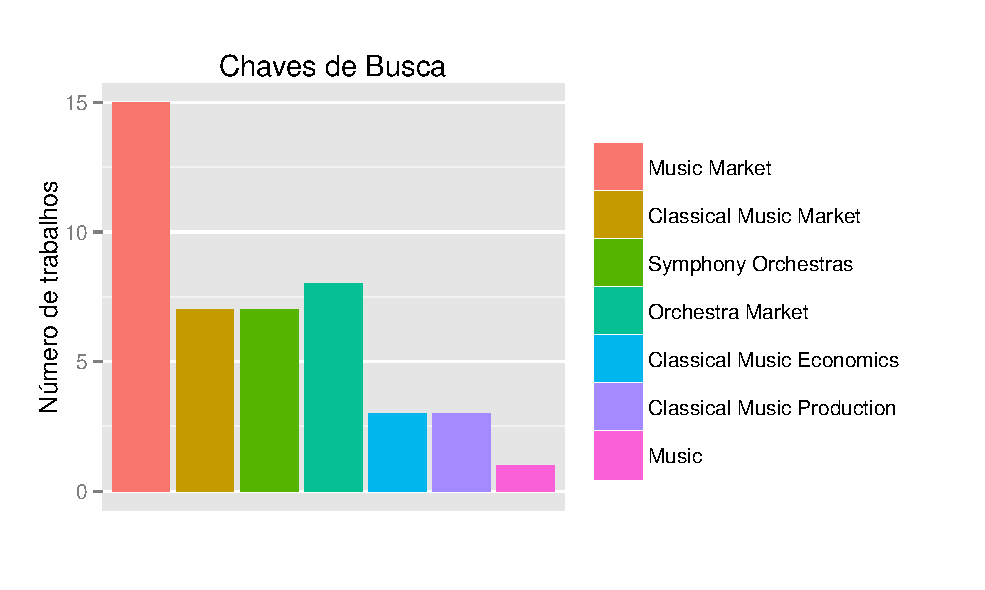
\includegraphics[scale=0.8]{chave.eps}
		\legend{Fonte: Dados trabalhados pelo autor}
	\end{figure}



	Dois estudos experimentais chamaram nossa atenção pela originalidade do desenho metodológico, a saber, \citeonline{salganik2008leading} pela aplicação do método experimental no estudo de um mercado cultural artificial e \citeonline{kasaras2012musical} que também utilizam do método experimental aliado à análise de redes sociais para investigar a influência no gosto musical na Web.  Eles são ainda bem recentes e não estão inseridos, como as outras metodologias, numa tradição de pesquisa em sociologia.

	Os métodos (cf. Tabela \ref{metodos-usados}) mais citados nos resumos foram a \textit{Social Network Analysis}, o \textit{Web-based Experiment} e pesquisas utilizando grandes bancos de dados (\textit{Big Data}) e entrevistas. Após cruzar as frequências dos métodos utilizados com o ano de publicação, investigamos se, de fato há associação entre essas variáveis na amostra calculando o $V$ de Cramér, uma medida para associação de variáveis categóricas. O $V$ de Cramér é definido por $$ V = \sqrt{\frac{\chi^2}{n\cdot(k-1)}} $$ onde $k$ é o menor valor entre o número de linhas e o número de colunas da tabela gerada \cite{barbetta2012estatistica}.

	O valor calculado para estas variáveis foi $V=0.9280$ indicando uma associação muito forte. As variáveis ``Métodos" e "Tipo de estudo" apresentaram associação perfeita. Podemos perceber que os métodos utilizados tem uma mudança mais significativa no tempo do que as metodologias propriamente. É notável a grande variedade de métodos utilizados nessa área de pesquisa. Esse fato aliado ao pequeno número de artigos publicados no espaço de trinta e um anos denota pouca atenção destinada ao campo do mercado da música de concerto o que, \textit{per se}, já justifica nosso esforço.



	% latex table generated in R 3.1.3 by xtable 1.7-4 package

	% Wed Jul 08 11:53:02 2015



	\begin{table}[ht]
		\ibgetab{
		\centering
		\caption{Tipos de Publicação}
	}
		{\begin{tabular}{lr}
			\hline
			\hline
			Artigo &  38 \\
			PhD Dissertation &   4 \\
			Livro &   2 \\
			\hline
			\end{tabular}
		}
		{\fonte{dados trabalhados pelo autor.}}
	\end{table}





	% latex table generated in R 3.1.3 by xtable 1.7-4 package

	% Wed Jul 08 11:56:08 2015

			\begin{table}[ht]
				\ibgetab{
				\centering
				\caption{Tipo de Estudo}
				\label{tipo-de-estudo}
			}
				{\begin{tabular}{lr}
					\hline
					\hline
					Case Study &   6 \\
					Experimental Study &   2 \\
					Estudo exploratório &   1 \\
					Estudo histórico &   6 \\
					Qualitativo &   1 \\
					Quantitativo &   5 \\
					Sociologia Econômica &   1 \\
					Institutionalist Economic Sociology &   1 \\
					\hline
					\end{tabular}
				}
				{\fonte{dados trabalhados pelo autor.}}
			\end{table}





	% latex table generated in R 3.1.3 by xtable 1.7-4 package

	% Wed Jul 08 11:57:57 2015

					\begin{table}[ht]
						\ibgetab{
						\centering
						\caption{Métodos usados}
						\label{metodos-usados}
					}
						{\begin{tabular}{lr}
							\hline
							\hline
							Multivariate Regression Analysis &   1 \\
							Big Data &   1 \\
							Big Data + Word Count &   1 \\
							Comparative Analysis &   1 \\
							Comparative Historical Analysis &   1 \\
							Discourse Analysis &   1 \\
							Método Econômico &   1 \\
							Field Theory / Organizational Theory &   1 \\
							Pesquisa Documental &   1 \\
							Racionalização &   1 \\
							Social Network Analysis &   3 \\
							Survey &   1 \\
							Web-based Experiment &   2 \\
							Interviews + Documentation Analysis + Statistics  &  1 \\
							Interviews + Music Journals + Promotional Literature &   1 \\
							\hline
						\end{tabular}
					}
					{\fonte{dados trabalhados pelo autor.}}
					\end{table}







	%				\begin{figure}

	%					\caption{Tipos de publicação e métodos utilizados por ano}

	%					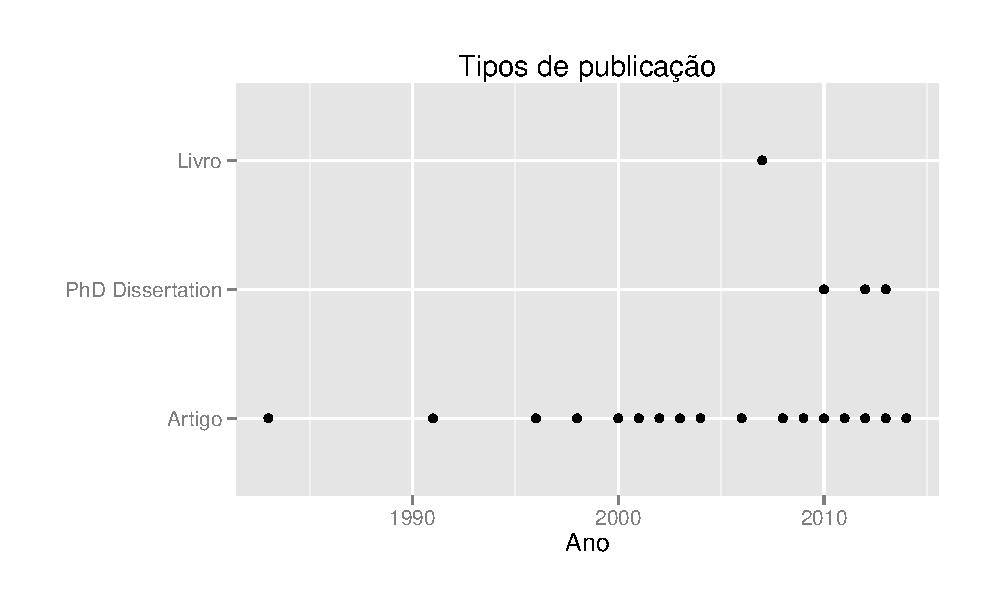
\includegraphics[scale=0.5]{tipopubano.eps}

	%					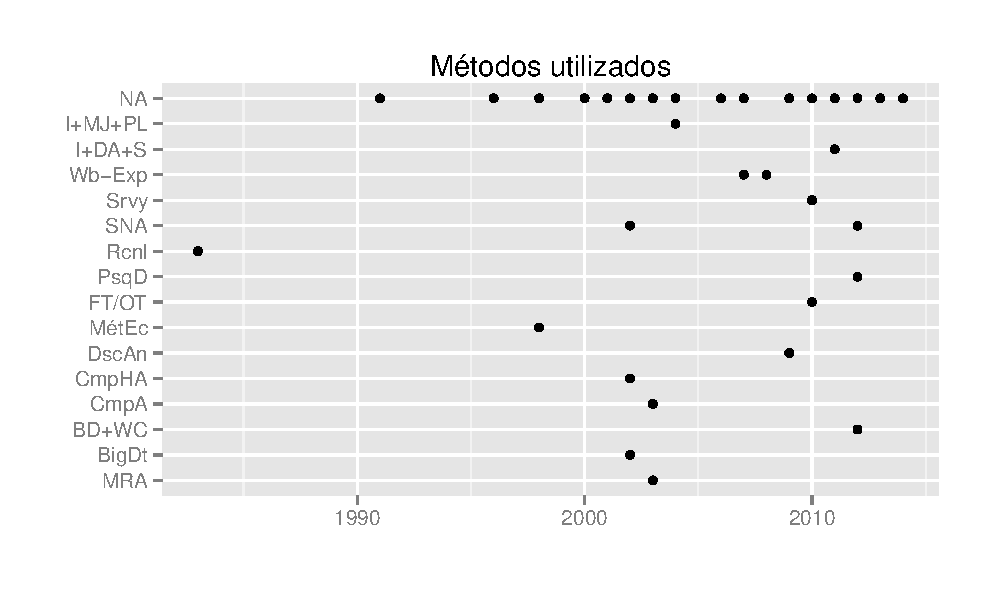
\includegraphics[scale=0.5]{metodoanoab.eps}

	%					\legend{Fonte: Dados trabalhados pelo autor}

	%				\end{figure}



	%\begin{figure}

	%	\caption{Métodos utilizados por ano}

	%	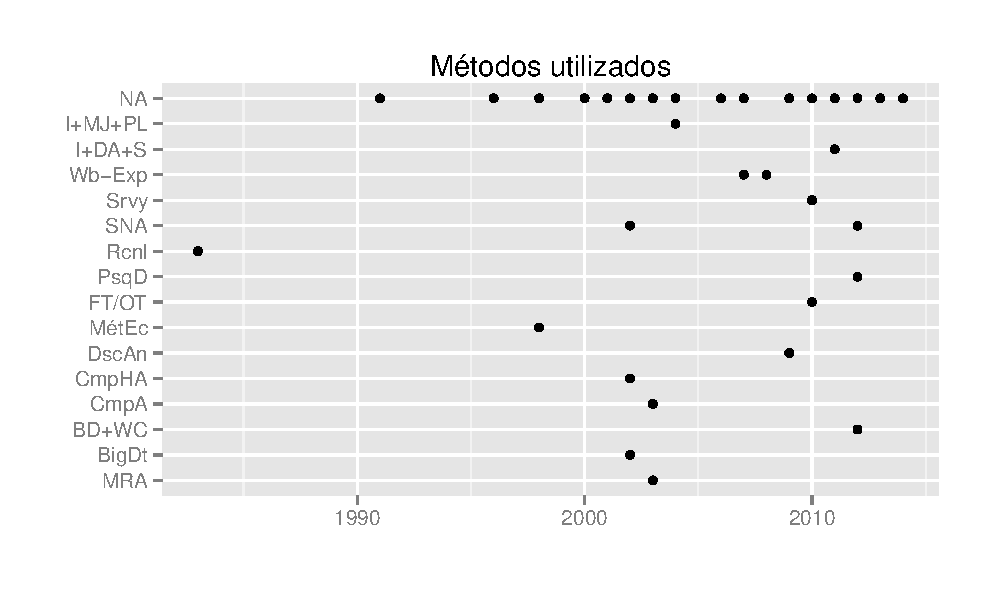
\includegraphics[scale=1]{metodoanoab.eps}

	%	\legend{Fonte: Dados trabalhados pelo autor}

	%\end{figure}



	%				\begin{figure}

	%					\centering

	%					\caption{Densidade de publicações por ano}

	%					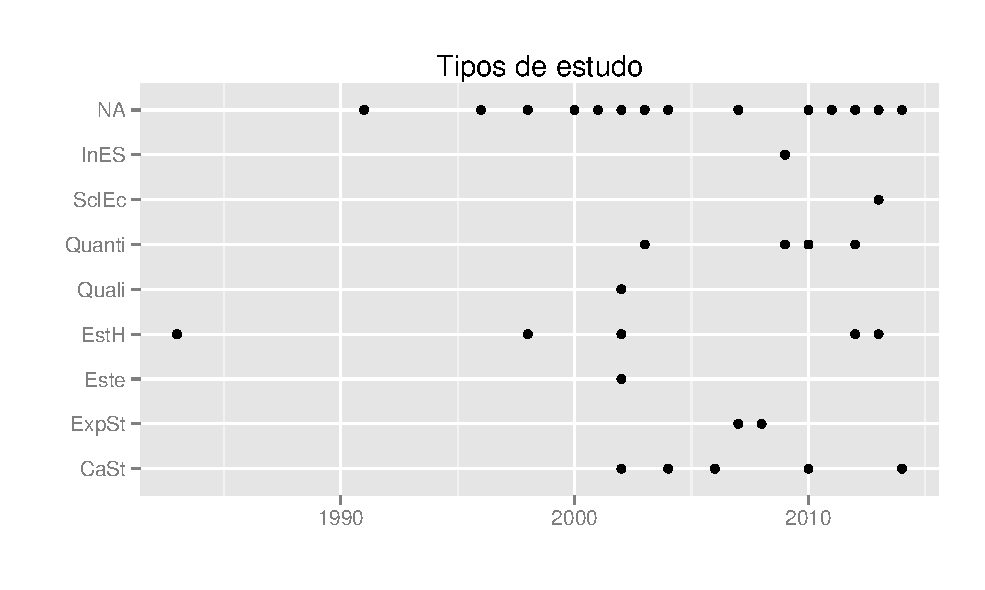
\includegraphics[scale=0.5]{tipoestudoano.eps}

	%					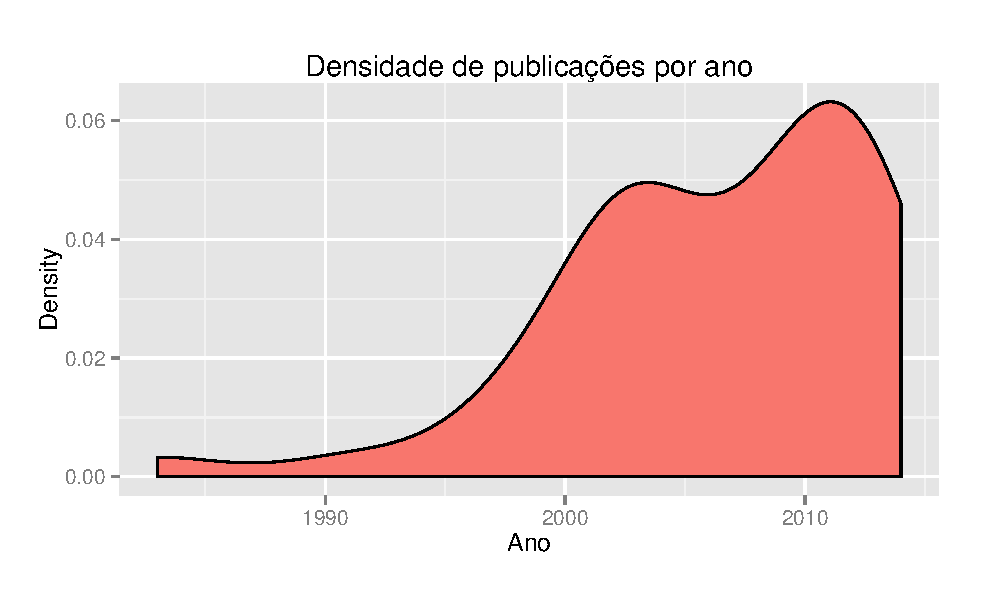
\includegraphics[scale=0.7]{anodensidade.eps}

	%					\legend{Fonte: Dados trabalhados pelo autor}

	%				\end{figure}



	O gráfico de densidade\footnote{Um gráfico de densidade mostra a propabilidade de as observações cairem numa janela de variação ao longo da variável de interesse. Em contraposição ao histograma que mostra uma medida discreta, o gráfico de densidade mostra um contínuo de distribuição dessas probabilidades \cite{lander2014r}.} na figura \ref{grafico-densidade} gerado a partir dos anos de publicação (Figura 3) mostra que, nos trinta e um anos analisados, o campo tem crescido. Este crescimento, entretanto, se deu mais efetivamente nos últimos quinze anos. A densidade das publicações até 1995 é bastante baixa.



	\begin{figure}
		\centering
		\caption{Densidade de publicações por ano}
		\label{grafico-densidade}
		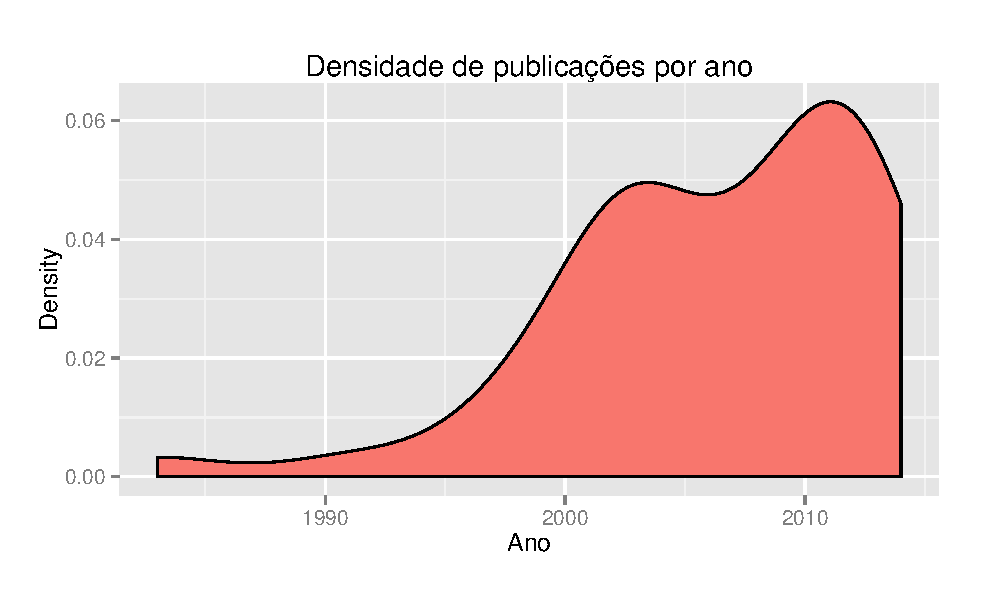
\includegraphics[scale=.6]{anodensidade.eps}
		\legend{Fonte: Dados trabalhados pelo autor}
	\end{figure}



		\section{Perspectivas teóricas e abordagens}

		Os temas de investigação aparecem nos trabalhos de uma maneira bastante difusa. Encontramos algumas publicações abordando aspectos culturais que influenciam o mercado da música, o mercado de trabalho dos músicos, as relações de gênero e a divisão do trabalho, financiamento e ``patronagem", o consumo da música e as variáveis que o explicam, gosto musical, padrões estéticos, identidade cultural e música nacional/folclórica, história social dos músicos, o ``cânon" do repertório musical, liderança do maestro e participação e satisfação dos músicos, música antiga\footnote{No campo da música, convencionou-se chamar de música antiga aquela escrita até o séc. XVII.}, revolução digital e indústria fonográfica.

		Percebemos algumas leves polarizações entre os autores expressamente citados nos resumos. Um deles é Bourdieu que, conhecidamente, deixou um vasto trabalho na área de sociologia da arte e do consumo de arte. O nome de Viviana Zelizer aparece relacionado ao de Bourdieu em um resumo consultado. Stigler e Becker são citados num trabalho que argumenta contra a perspectiva econômica neoclássica. Matthew Salganik também aparece nessa bibliografia como autor de dois trabalhos e é citado por mais um indicando novamente atenção ao método experimental na área. No campo, alguns trabalhos tendem a seguir uma perspectiva teórica que privilegia a influência dos aspectos culturais na economia (sociologia econômica). No entanto, não há uma corrente teórica definida perceptível, o que indica que a área não é madura e nem tem uma tradição de pesquisas consolidada.

		No primeiro anexo deste trabalho apresentamos para o leitor um quadro contendo autor, ano, periódico de publicação e principais assuntos de todos os trabalhos aqui investigados. Pelo fato de que todas referências encontradas são apenas tangenciais ao nosso objeto de pesquisa, nenhuma delas foi revisada em profundidade. O mérito desta investigação bibliográfica preliminar reside justamente no reconhecimento de que nosso objeto de pesquisa permanece até hoje praticamente inexplorado em suas particularidades.





	\chapter{Os produtos culturais}

	O primeiro desafio deste trabalho reside no fato de que estamos lidando com um objeto que desafia a maioria dos pressupostos da teoria econômica vigente. Comecemos, portanto, estabelecendo algumas diferenças fundamentais entre os bens culturais e as mercadorias comuns conforme concebidos tradicionalmente pela teoria econômica. Segundo \citeonline{tolila2007cultura}, as mercadorias são entendidas por meio de quatro critérios objetivos, a saber, suas propriedades físicas (as quais, nesse caso, estão diretamente relacionadas com a qualidade do produto em questão), a data e o local em que ele está disponível e aquilo que condiciona sua entrega num universo certo, i.e., sem incertezas. A qualidade de um bem, nessa perspectiva, pode ser decomposta em uma série de elementos objetivos, i.e., claramente mensuráveis e hierarquizáveis. Além disso, na teoria econômica clássica todo bem é considerado um ``bem privado'' e, portanto, ``exclusivo e rival'' no consumo. Para citar um exemplo, ``um café, um sanduíche, uma camisa, um par de sapatos, uma cadeira, etc., são bens exclusivos porque é possível impedir-me de obtê-los (\ldots); por outro lado, cada um desses bens é de consumo exclusivo porque no momento em que o aproveito, nenhuma outra pessoa pode usufruí-lo'' \cite[p. 29]{tolila2007cultura}. Ora, os produtos culturais, de um modo geral, são não exclusivos; pode-se, por exemplo, admirar um belo edifício histórico na rua sem ter que pagar por isso. Tampouco são rivais no consumo; o prazer de assistir um concerto não é diminuído pela presença de outras pessoas no público.

	Esse setor da economia define-se, ainda, pela sua lógica de oferta voltada à produção, ao contrário dos mercados de bens comuns voltados ao consumo. Para \citeonline[p. 32]{tolila2007cultura}, ``essa lógica da oferta caracteriza bem, entre outras, a ação das políticas públicas em termos de investimento, de ajuda e de sustentação das atividades culturais, do patrimônio ao espetáculo ao vivo, e em termos de incentivos às práticas culturais''. De fato, os Estados e coletividades públicas tem demonstrado interesse crescente no setor cultural, o que pode ser verificado através das políticas públicas, das administrações especializadas, da alocação de recursos dirigidos especificamente ao setor e do surgimento de toda uma rede de instituições e profissionais atuantes no setor cultural, grande parte deles financiados por dinheiro público \cite{tolila2007cultura}. Para \citeauthoronline{tolila2007cultura}

	\begin{citacao}
		Consequentemente, a atenção das autoridades, dos cidadãos e de seus representantes, foi desenvolvida em duas direções clássicas no contexto das democracias: por um lado, \textbf{o debate público interno} sobre a alocação dos recursos, o valor deles e seu significado, por outro, \textbf{a competição exterior} com os outros Estados pelas questões de mercados e de comércio. Essa segunda direção (\ldots) é inseparável dos dilemas e debates que movimentam atualmente todas as reflexões sobre \textbf{a globalização e a diversidade das expressões culturais}. \cite[p. 71-2]{tolila2007cultura}
	\end{citacao}

	Para esse autor, esses dois elementos são constitutivos do valor simbólico atribuído às práticas e ao desenvolvimento cultural à medida que traz relevância ao debate relacionado à identidade e diversidade cultural. O valor simbólico dos bens culturais constitui, para nós, um elemento central na compreensão de nosso objeto de estudo, muito embora, contrariando novamente a teoria econômica clássica, não seja objetivo em sua natureza mas relacional e individual, i.e., só existe à medida que é reconhecido pelo indivíduo no momento de seu consumo. Para que o valor simbólico de um determinado bem seja reconhecido, é necessário que haja estruturas cognitivas apropriadas para a compreensão e fruição do bem, ou seja, esquemas mentais adquiridos por meio da educação artística prévia \cite{bourdieu2003amor}.

	As performances musicais possuem ainda uma particularidade quanto à natureza de sua existência na qual reside grande parte das dificuldades metodológicas que as cercam. \citeonline{tolila2007cultura} explica:

	\begin{citacao}
		O que é a música? A partitura escrita? Não. Os músicos que formam a orquestra? Não. O regente? Também não. Na verdade, é quase impossível definir a música como uma ``coisa'' (uma mesa, uma cadeira, uma casa, etc.) pois ela só existe de fato no momento em que é ouvida, isto é, em uma relação com o ouvinte\footnote{Para o autor, ``na verdade, no mundo social, o modo real de existência da maioria dos fenômenos é o da relação entre seres humanos'' \cite[p. 110]{tolila2007cultura}. Curiosamente, nessa premissa se baseia todo o paradigma neoestrutural na sociologia conhecido também como ``perspectiva relacional'' ou ``teoria das redes sociais''.}. \cite[p. 109]{tolila2007cultura}
	\end{citacao}

	Desse modo, a música (bem como a dança e o teatro, por exemplo) assume um modo especial de existência que envolve a participação de todos os elementos ou atores supracitados, a saber, partitura, músicos, regente, etc., na construção de sua materialidade que só existe (e portanto só é possível de ser consumida) no momento da escuta. Segundo \citeonline[p. 54]{benhamou2007economia} ``a concorrência assume a forma paradoxal de uma competição entre instituições que oferecem bens únicos e efêmeros'' onde o comportamento dos atores econômicos tende a monopólios discriminatórios. Para essa autora, o setor é caracterizado por uma fragilidade constante devido a elevações periódicas de custos e à quase-ausência de reservas de produtividade. De fato, como veremos, o paradigma vigente, no que tange a teoria econômica das performances ao vivo, aponta para um inevitável estado deficitário.
	
	\section{A economia das singularidades}
	
	 %\citeonline{karpik2009elements,karpik2007economie} addresses the problem of stating a market for the ``good'' musical interpretation as well as the good lawyer, wine, theatre spectacle, concert, etc. How something that is, in essence, not comparable and incommensurable can delineate a market?
	
	\citeonline{karpik2009elements,karpik2007economie} abordam o problema do estabelecimento de um mercado da ``boa''interpretação musical bem como do bom advogado, do bom vinho, do bom espetáculo teatral, do bom concerto, etc. Como algo que é, em essência, não comparável e incomensurável pode delinear um mercado?
	
	%\citeonline{karpik2009elements} states that this problem is resolved with the \textit{judgement devices}. To understand the judgement devices, it is necessary to point the basic difference between the \textit{decision} and the \textit{judgement}. The former is essentially made upon calculations aiming for the optimal outcome. The latter is related to the qualities of a given product and its main action is the \textit{choice}. To this author, no calculation would help on choosing between, say, the best interpretation of Beethoven's 5th. The choice is made essentially as a judgement, an arbitrary and subjective action that tries to take into account all the information one can dispose to build knowledge that differentiates the options into a practical way. For the judgement to happen, consumers mobilize five kinds of judgement devices: (1) networks, the only personal device and the other impersonal devices  (2) appellations, (3) cicerones, (4) rankings and (5) confluences.
	
	\citeonline{karpik2009elements} coloca que esse problema é resolvido através de \textit{dispositivos de julgamento}\footnote{Judgement devices.}. Para entender os dispositivos de julgamento, é necessário apontar a diferença básica entre a \textit{decisão} e o \textit{julgamento}. O primeiro é essencialmente formado a partir de cálculos que visam o \textit{outcome} ótimo. O último está relacionado às qualidades de um dado produto e sua ação principal é a \textit{escolha}. Para esse autor, nenhum cálculo poderia ajudar na escolha, digamos, da melhor interpretação da Quinta Sinfonia de Beethoven. A escolha é feita essencialmente como um julgamento, uma ação arbitrária e subjetiva que tenta levar em conta toda a informação de que se dispõe para construir conhecimento que diferencie as opções de uma maneira prática. Para que o julgamento aconteça, os consumidores mobilizam cinco tipos de dispositivos de julgamento: (1) as redes, o único dispositivo pessoal, e os dispositivos impessoais (2) apelações, (3) cicerones, (4) rankings e (5) confluências.
	
	
	EXPLICAR.......................................
	
	
	
	CONECTAR................
	
	%According to \citeonline[p. 54]{benhamou2007economia}, ``competition takes a paradoxical form of a competition between institutions that offer unique and ehpemeral goods'' where economic actors behavior tend to discriminatory monopolies. According to the author, the sector is characterized by a strong inclination to the singularities and a constant fragility because of periodic cost increases and the nearly absence of productivity reserves. In fact, as we will see, the current paradigm, regarding the economic theory of live performances, points to an inevitable deficit. We will now examine these two points in further detail.
	
	De acordo com \citeonline[p. 54]{benhamou2007economia}, ``a competição toma uma forma paradoxa de uma competição entre instituições que oferecem bens únicos e efêmeros'' onde o comportamento dos atores econômicos tende a monopólios discriminatórios. De acordo com a autora, o o setor é caracterizado por uma forte inclinação às singularidades e uma fragilidade constante devido aos aumentos de custo periódicos e a quase ausência de reservas de produtividade. De fato, conforme argumentação que será apresentada abaixo, o paradigma corrente com relação à teoria econômica da performance ao vivo aponta para o déficit inevitável. Examinaremos agora esses pontos em maiores detalhes.
	

	\section{O modelo de Baumol e Bowen -- a ``doença dos custos''}

	William Baumol e William Bowen empreenderam, sob encomenda da Fundação Ford em 1965, uma pesquisa visando diagnosticar a situação econômica dos teatros da Broadway \cite{benhamou2007economia}. Seus achados são até hoje considerado válidos. Para \apudonline{baumol1966performing}{benhamou2007economia} a economia divide-se em dois setores, o setor 1 (arcaico) e o setor 2 (progressista). O setor arcaico não apresenta possibilidades de gerar ganhos de produtividade enquanto o setor progressista gera ganhos de produtividade a partir de inovações, de economias de escala e da acumulação de capital. A performance ao vivo faz parte do setor arcaico e isso se deve à posição que nele ocupa o trabalho. Para \citeonline{benhamou2007economia}

	\begin{citacao}
		O trabalho é um elemento constitutivo do produto final: não se poderia substituí-lo sem desnaturar o produto. Não se poderia, por exemplo, substituir um dos instrumentistas de um quarteto de cordas por uma gravação\ldots Ora, os salários são iguais aos do setor progressista, devido à fluidez do mercado de trabalho; a consequência é um aumento permanente dos custos relativos do espetáculo ao vivo, que somente uma elevação dos preços das entradas pode compensar, com o risco de reduzir a demanda e as receitas.
	\end{citacao}

	O modelo de \apudonline{baumol1966performing}{benhamou2007economia} baseia-se nas três hipóteses que se seguem:

	\begin{enumerate}
		\item A economia divide-se em dois setores, arcaico e progressista. No setor arcaico, onde reside a performance ao vivo, a produtividade do trabalho é constante ou aumenta pouco e a quantidade de trabalho não pode ser diminuída sem desnaturar o produto. Sendo $L_{1,t}$ o volume de trabalho empregado no setor 1 no momento \textit{t} e \textit{a} um valor constante, a quantidade de produto no setor 1 no momento \textit{t} ($Y_{1,t}$) é obtida por $$Y_{1,t} = aL_{1,t}$$

		Sejam $Y_{2,t}$ e $L_{2,t}$ respectivamente a quantidade de produto do setor progressista no momento \textit{t} e o volume de trabalho empregado no setor 2 no momento \textit{t}, seja r a taxa de aumento da produtividade do trabalho e \textit{b} uma constante, a quantidade de produto no setor é obtido por $$Y_{2,t} = bL_{2,t}[1+r]^t $$

		\item Os custos de produção, comparados somente com os custos salariais (\textit{W}), evoluem no mesmo ritmo e sentido que a produtividade no setor progressista, isto é, $W_{1,t} = W_{2,t} = W_t = W[1+r]^t$. Os custos relativos de cada setor são, portanto, dados por
		$$C_1 = \frac{W_tL_{1,t}}{Y_{1,t}} = \frac{W(1+r)^tL_{1,t}}{aL_{1,t}} = \frac{W(1+r)^t}{a}$$
		$$C_2 = \frac{W_tL_{2,t}}{Y_{2,t}} = \frac{W(1+r)^tL_{2,t}}{bL_{2,t}(1+r)^t} = \frac{W}{b}$$

		Tem-se, então, que o custo por unidade de produto obtido aumenta indefinidamente no setor 1 e mantém-se constante no setor 2. As funções de custos de produção em ambos os setores está representada na Figura \ref{custos-de-producao}.

		% Inserir a figura plotando as duas funções
		\begin{figure}[!h]
			\centering
			\caption{Custos de Produção}
			\label{custos-de-producao}
			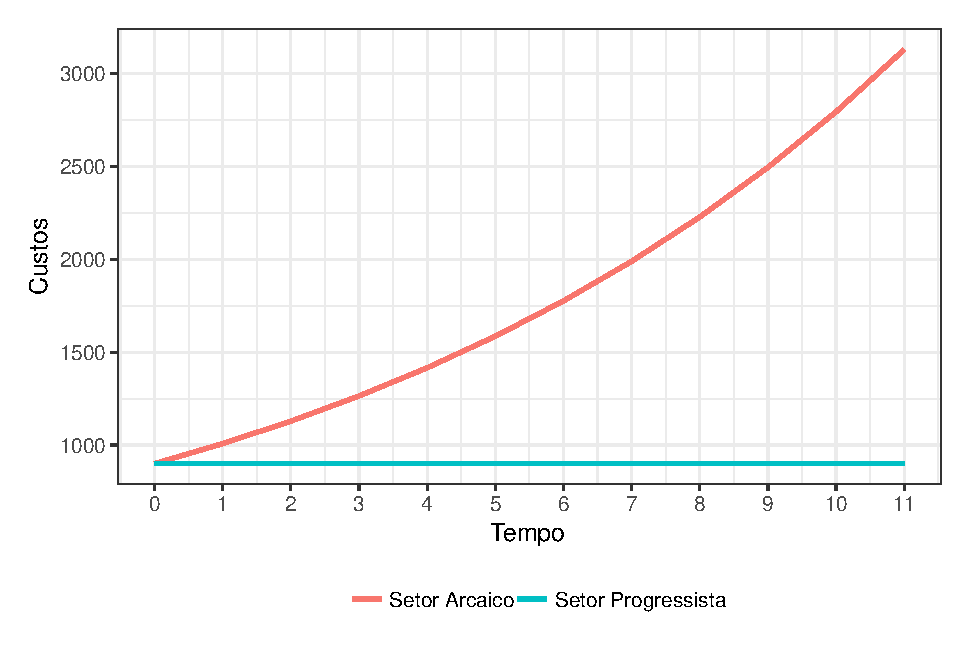
\includegraphics[scale=1]{doenca_dos_custos.eps}
			\fonte{Elaboração do autor.}
		\end{figure}


		\item ``A demanda de espetáculos ao vivo é elástica; toda alta de preço redunda numa redução do público'' \cite[p. 56]{benhamou2007economia}. Sendo os preços proporcionais aos custos relativos nos dois setores, $P_1 = \alpha C_1$ e $P_2 = \beta C_2$, então
		$$\frac{P_1Y_1}{P_2Y_2} = \frac{\alpha C_1Y_1}{\beta C_2Y_2} = Cte$$ ou
		$$\frac{C_1Y_1}{C_2Y_2} = \frac{W(1+r)^t \cdot L_{1,t}}{W(1+r)^t \cdot L_{2,t}} = \frac{L_{1,t}}{L_{2,t}} = K_0$$ e
		$$\frac{Y_1}{Y_2} = \frac{aL_{1,t}}{bL_{2,t}(1+r)^t} = \frac{aK_0}{b(1+r)^t}$$

		``Quando \textit{t} aumenta, $\frac{Y_1}{Y_2}$ diminui, e quando $t \rightarrow \infty$, $\frac{Y_1}{Y_2} \rightarrow 0$'' \cite[p. 57]{benhamou2007economia}. Desse modo, a produção do setor arcaico (1) diminui fatalmente.
	\end{enumerate}

	De forma complementar à lei de Baumol, \citeonline{throsby1994production} desenvolve uma função da produção do espetáculo ao vivo a qual pode ser sintetizada da seguinte forma:

	O número de representações de uma determinada temporada deve ser fixado levando em conta a capacidade da sala \textit{v}. Sejam $L^s$ e $K^s$ o trabalho e o capital necessários para montar uma produção, sejam $L^r$ e $K^r$ o trabalho e o capital requeridos por cada representação da produção, o número de espectadores da iésima representação da jésima produção, $y_{ij}$, tal que $y_{ij} \leq v$, é dado por
	$$y_j = \sum_iy_{ij} = y_i(L^{s}_{j}, K^{s}_{j}, m_j, q_j) $$ onde
	o número de representações da jésima produção $$m_j = m_j(L^{r}_{j}, K^{r}_{j})$$ e $q_j$ resume as qualidades da jésima produção as quais, nesse contexto, podem ser medidas pela luxuosidade (\textit{lavishness}) da produção. Nesse caso, $q_j$ não é independente de $L^s$ e $K^s$. Espera-se que $$\frac{\partial y_j}{\partial m_j} > 0 \quad, \quad \frac{\partial^2y_j}{\partial m^{2}_{j}} < 0,$$ isto é, extender a temporada pode reduzir o número de espectadores na margem.

	Segundo \citeonline[p. 59]{benhamou2007economia} ``a conclusão do modelo [de Baumol] é a inelutabilidade do aumento dos déficits dos espetáculos ao vivo''. Esse modelo tem sido corroborado por várias pesquisas \cite[e.g.]{throsby1979economics,leroy1980economie,peacock1983inflation,baumol1984inflation,dias2011artes} e, para \citeonline[p. 54]{benhamou2007economia}, essa característica do setor é suficiente para justificar o aumento das subvenções públicas e da prática do mecenato mesmo tendo em vista que ``essa intervenção maciça, distribuída de forma muito desigual, não é suficiente para garantir ao setor um equilíbrio financeiro duradouro''. Para \apudonline[p. 320]{baumol1966performing}{luksetich2011orchestras}, ``se se concorda que a artes de performance conferem benefícios gerais à comunidade como um todo\ldots as artes são bens públicos cujos benefícios demonstravelmente excedem as receitas que se espera coletar na bilheteria\footnote{If one agrees that the performing arts confer general benefits on the community as a whole\ldots the arts are public goods whose benefits demonstrably exceed the receipts one can hope to collect at the box office.}''. O modelo, entretanto, possui inconsistências, algumas delas apontadas por \citeonline{benhamou2007economia}.

	A primeira consiste do pressuposto de que os salários do setor 1 são iguais aos do setor 2. Entretanto, desde a Segunda Guerra Mundial, os salários médios no setor do espetáculo ao vivo apresentaram uma tendência a crescerem menos do que no outro setor \apud{throsby1994production}{benhamou2007economia}. A segunda consiste do pressuposto altamente discutível de que a demanda é sensível ao preço. Maior parece ser o efeito da qualidade (percebida) do espetáculo sobre a demanda. De fato, \citeonline{throsby1994production} salienta que, por causa da dificuldade na medição da qualidade das performances, os efeitos dessa variável usualmente ficam restritos ao termo do erro nos modelos econométricos com a exceção de um estudo experimental conduzido pelo próprio \citeonline{throsby1983quality}. Nesse trabalho, o autor identificou algumas características da qualidade da performance no teatro como a qualidade da atuação, da produção, do roteiro e encontrou que a demanda é inelástica com relação ao preço dos ingressos mas \textit{altamente correlacionada com a qualidade esperada}. Este ponto parece central na investigação do mercado das orquestras e será desenvolvido oportunamente.

	Além disso, é possível reduzir os custos de uma produção de espetáculo ao vivo de várias formas, a saber, através da gravação e reprodução do espetáculo, através do uso, na música, de sons \textit{sampleados} ou eletrônicos ao invés da contratação de músicos, a utilização de um mesmo ator representando mais de um papel em uma montagem cênica ou a reutilização de cenários e figurinos (práticas comum em montagens modernas de ópera), dentre várias outras. Para \citeonline[p. 60]{benhamou2007economia} esses meios ``equivalem a substituir o déficit comercial por um `déficit artístico'. Mesmo assim, essas medidas não são suficientes para compensar a diferença de produtividade.

	A terceira inconsistência reside no fato de que a alta da produtividade nos setores progressistas acompanhada por um aumento de salário proporcional à melhora das qualificações provoca um crescimento da procura por espetáculos, o que \textit{per se} contribui com a solução das dificuldades criadas pela diferença de produtividade nos setores \apud{throsby1979economics}{benhamou2007economia}. O crescimento, para \apudonline{baumol1966performing}{benhamou2007economia} reside na presença de consumidores cada vez mais sagazes e exigentes e acaba por gerar custos marginais superiores às receitas. ``As companhias musicais ajudaram a construir a reputação de artistas cuja contratação se tornou inevitável. A consequência é um aumento exagerado dos cachês e dos custos'' \cite[p. 61]{benhamou2007economia}.

	Por mais que seja verdadeira esta última constatação sobre os custos gerados na contratação de artistas de renome, parece também uma grande ingenuidade acreditar que o aumento de salário acarreta um crescimento na procura por espetáculos ao vivo. Na verdade os estudos em sociologia econômica tem mostrado, como veremos, que o consumo artístico está ligado ao que Bourdieu (\citeyear{bourdieu2011forms,bourdieu2003amor,bourdieu2007distincao}) chama de ``capital cultural'' e à construção de uma identidade social.

	A quarta inconsistência é esta: A gravação dos espetáculos pode gerar receita. Embora as rendas de espetáculos gravados sejam pequenas conforme investigações no contexto americano \apud{heilbrun2001economics}{benhamou2007economia} parecem ser um recurso bastante explorado no setor Algumas orquestras brasileiras costumam disponibilizar as gravações de seus concertos e óperas como produto secundário da sua carta de produtos. Gravações de estúdio e ainda outros produtos (camisetas, acessórios, \textit{souvenirs}) compõem o financiamento dessas instituições. Oportunamente abordaremos esse ponto.

	\citeonline{throsby1994production}, após revisar vários estudos que testam a lei de Baumol conclui que

	\begin{citacao}
		Os impactos combinados dos ajustes de produção aumentaram a demanda e níveis crescentes de receita não esperada contrariaram qualquer tendência em direção a um aumento secular nos déficits entre companias de performance sugerindo que, embora a doença dos custos irá indubitavelmente continuar a presentear a artes performáticas com problemas difíceis, é improvável que chegue ao extremo\footnote{the combined impacts of production adjustments increased demand, and generally rising levels of unearned revenue have countered any tendency towards a secular rise in deficits among performance companies, suggesting that although the cost disease will doubtless continue to present the performing arts with difficult problems, it is unlikely to be terminal.}. \cite[p. 16]{throsby1994production}
	\end{citacao}

	Por fim, a análise de \citeonline{baumol1966performing} apontando a especificidade do setor contribuiu tanto para o desenvolvimento do programa de pesquisa que hoje conhecemos como economia da cultura quanto para o reconhecimento da necessidade de vinculação dos espetáculos ao vivo à esfera não-comercial subvencionada. Sigamos agora examinando como o mercado cultural brasileiro obtém seus recursos e o principal mecanismo de financiamento para que isso aconteça: as leis de incentivo à cultura.

	\section{Políticas Culturais no Brasil}

	Para \citeonline[p. 62]{benhamou2007economia}, ``na França, o espetáculo ao vivo vive essencialmente das subvenções públicas''. A realidade brasileira não parece ser diferente. No Brasil, a música de concerto, bem como as artes em geral, parecem obter a maior parte de seu financiamento através do Estado seja por investimento direto, seja por investimento indireto via isenção fiscal. No contexto brasileiro, a mais substantiva política pública na área da cultura reside na implementação de mecanismos de fomento à produção cultural mediante isenção fiscal os quais conhecemos como ``leis de incentivo à cultura''. Para \citeonline{sarkovas2005incentivo} a receita dos empreendimentos culturais \textit{per se} não dão conta de suprir as demandas do setor. Por isso se fazem necessárias outras três fontes de financiamento, a saber,

	\begin{citacao}
		\_o Estado, que tem a responsabilidade de fomentar a criação artística e intelectual, e a distribuição do conhecimento, bases do progresso humano;\\
		\_o investimento social privado, evolução histórica do mecenato, meio pelo qual cidadãos e instituições privadas tornam-se agentes do desenvolvimento da sociedade;\\
		\_o patrocínio empresarial, estratégia de construção de marcas e de relacionamento com seus públicos, feita por associação com ações de interesse público. \cite[p. 22]{sarkovas2005incentivo}
	\end{citacao}

	Para \citeonline{sarkovas2005incentivo}, essas três fontes foram interconectadas na criação de um sistema de financiamento por isenção fiscal que culminou em nossa conhecida Lei de Incentivo à Cultura. Em 2 de julho de 1986 era sancionada a ``Lei Sarney'', o primeiro mecanismo de isenção fiscal do país. Essa lei permitia que contribuintes abatessem dos impostos a pagar parte da quantia que decidiram investir em instituições culturais. A lei foi revogada sem motivo aparente em 1990 dando lugar a iniciativas semelhantes organizadas pelos governos municipais. No fim do mesmo ano foi promulgada em São Paulo a ``Lei Mendonça'' que permitia dedução do ISS\footnote{Imposto sobre serviços de qualquer natureza.} e do IPTU\footnote{Imposto sobre propriedade predial e territorial urbana.}. Outros municípios brasileiros acompanharam a medida e alguns estados criaram um modelo de isenção fiscal cujo abatimento se dava sobre o ICMS\footnote{Imposto sobre a circulação de mercadorias e serviços.}. Em dezembro de 1991 o sociólogo e então secretário da cultura Sérgio Paulo Rouanet instaura o ``Programa Nacional de Apoio à Cultura'' que ficou conhecido como Lei Rouanet. O programa instituía os mesmos mecanismos de isenção fiscal da antiga Lei Sarney e instituía ainda dois novos instrumentos, o FNC (Fundo Nacional de Cultura) e o FICART (Fundos de Investimento Cultural e Artístico). Segundo \citeonline{sarkovas2005incentivo}, nenhum dos dois mecanismos vingou. Para ele,

	\begin{citacao}
		O FICART tornou-se letra morta porque seus benefícios foram largamente superados pelos níveis de dedução fiscal obscenos que seriam depois adotados em outros mecanismos. E o FNC jamais foi operado pelas regras primárias de um fundo público: transparência de critérios, acessibilidade paritária e primazia do mérito público. Desde que foi criado, seus recursos são arbitrariamente distribuídos segundo predileções e interesses do Ministério da Cultura. \cite[p. 22-3]{sarkovas2005incentivo}
	\end{citacao}

	Em 1997 a medida provisória 1.589 introduziria a dedução de 100\% para as áreas de artes cênicas, livros de valor artístico, literário ou humanístico, música erudita ou instrumental, circulação de exposições de artes plásticas e doações de acervos para bibliotecas públicas e para museus. Em sua gestão, o ministro da cultura Gilberto Gil iniciou um processo de consulta pública em diversos estados denominado ``Cultura para Todos'' visando aprimorar a Lei Rouanet. Para \citeonline{sarkovas2005incentivo}, apesar das boas intenções, a medida foi realizada sem planejamento estratégico adequado e falhou em prover soluções para os problemas encontrados no modelo de financiamento. Esses problemas se relacionam sobretudo ao modo de seleção de projetos a serem financiados pela lei o qual reside na iniciativa privada. Nas palavras desse autor,

	\begin{citacao}
		O financiamento por dedução fiscal transfere e pulveriza, aleatoriamente, o dinheiro e a responsabilidade pública para as empresas e por	isso não é o instrumento adequado para produzir os efeitos que Gil alega desejar: ``desconcentração e democratização dos recursos; ampliação da responsabilidade do Estado e do público beneficiado; qualificação do processo de seleção dos projetos; facilitação e	apoio aos pequenos empreendedores; desburocratização e melhoria dos instrumentos de gestão”. Seria mais eficaz, e menos demagógico, estudar os modelos de financiamento público	direto que funcionam, no Brasil e no mundo,	dentro e fora da área cultural. \cite[p. 25]{sarkovas2005incentivo}
	\end{citacao}

	Isso acontece porque, apesar de o financiamento acontecer através de isenção fiscal, ou seja, com dinheiro público, são as empresas privadas que selecionam os projetos nos quais pretendem ``investir''. Para \citeonline[p. 27]{sarkovas2005incentivo} ``empresas patrocinam para ampliar sua credibilidade, estimular a identificação e melhorar o relacionamento com seus públicos de interesse; agregar atributos e valorizar suas marcas; demonstrar sua participação social''. Desse modo, projetos com grande mérito artístico, cultural ou pedagógico seriam suplantados por projetos que tenham maior apelo de mercado ou que se identifiquem mais com o público alvo da empresa patrocinadora. Para \citeonline[pos. 524]{weiss2009estatais}, um dos pontos fracos da Lei Rouanet consiste justamente da ``desproporção de apoio entre projetos grandiosos e de entretenimento -- e, portanto, de grande apelo de marketing -- e projetos locais, ligados à formação'' além do baixo retorno de captações. Os autores argumentam que mesmo sendo o principal motor da atividade cultural no país tendo movimentado em 2008 cerca de R\$ 1,4 bilhão, o mecanismo gera desequilíbrios, visto que ``as empresas habituaram-se a patrocinar com dinheiro público e os produtores culturais a contar com essa captação como única alternativa''\cite[pos. 475]{weiss2009estatais}.


	No Brasil, o Estado aparece como a grande instituição financiadora e mantenedora da arte, seja através de investimentos diretos, seja por investimentos indiretos. Em outros países, entretanto, encontramos cenários diversos. Alguns divergem completamente onde o financiamento da cultura é focado no mercado e as instituições culturais preferem não se submeter às regras impostas pelo Estado, outros assemelham-se ao caso brasileiro embora com uma porcentagem muitíssimo menor de financiamento público. \citeonline{van2006making} estudou as diversas formas de intervenção estatal nas artes no contexto europeu e avaliou as asserções comuns no discurso da área que sustentam a legitimidade/necessidade dessa intervenção conceituando as diversas linguagens artísticas como bens públicos ou não.


	Após as considerações sobre as especificidades dos produtos culturais e uma investigação preliminar sobre o modelo de financiamento da cultura vigente no Brasil apresentados acima, revisaremos agora a base teórica escolhida para análise. Tentaremos construir um \textit{framework} teórico dentro da teoria social que leve em conta os achados que apresentamos até agora. Começaremos apresentando cada um dos elementos que vamos agregar em nossa análise, a saber, (1) o modelo $W(y)$ de White, (2) a teoria de Fligstein, (3) os isomorfismos normativos e (4) as redes multinível.
	
	%Baumol's analysis pointing the specificities of the cultural sector contributed to both the development of the research program that we know today as economy of culture and the recognition of the necessity of binding live performances to the subsidized non-commercial sphere. However, this approach is a standard economic one which, for the purposes of this investigation, lacks some of the social elements that are important to understand the shaping of a market, namely, institutions, social control, cooperation and social coordination, etc. Therefore, we will now try to build a theoretical framework inside social theory and accounting for the findings we have seen so far. Let us start presenting each of the elements we are going to aggregate in our analysis framework, namely, (1), White's $W(y)$ model, (2), Fligstein's theory, (3), normative isomorphisms and (4) multilevel networks.



	\chapter{A Construção Social dos Mercados}

	%Para entender o mercado da música de concerto, é necessário um arcabouço teórico que o dê sentido e, ao mesmo tempo, conduza o olhar do pesquisador. No processo de pesquisa, foi possível identificar elementos de diversos \textit{frameworks} teóricos que lançam luz sobre o nosso objeto de estudo. Neste capítulo, nosso esforço se dará numa tentativa de articulação desses elementos de modo a obtermos um arcabouço teórico para análise de nosso objeto. Apresentaremos quatro elementos teóricos que lidam com a emergência dos mercados, a saber, o modelo relacional de Harrison White, o modelo de Fligstein, o conceito de \textit{coopetition} e o conceito de isomorfismos organizacionais.

	\section{O modelo de White}

	Para Harrison \citeonline{white2002markets}, os mercados não são dados mas são estruturas sociais que emergem de interações complexas de seus componentes. Essas interações podem acontecer tanto de forma competitiva quanto, argumentamos, de forma cooperativa visando estabilização do mercado e redução do que o professor White chama de ``incerteza knightiana\footnote{Em referência ao economista americano Frank H. Knight.}''.

	Sua teoria visa explicar ``como as firmas minimizam incertezas formando um mercado como uma coleção de nichos baseada em sinais observados em seus engajamentos\footnote{(...) how firms minimize uncertanty by forming a market as a collection of niches based on signals observed in their commitments.}'' \cite[p. xiii]{white2002markets}. Em que consiste, portanto, um mercado de produção? A resposta para essa pergunta perpassa duas dimensões. A primeira, já comentada no parágrafo acima, remonta à natureza interdependente de sua estrutura, ou seja, uma emergência a partir das dependências de seus próprios fluxos. A segunda remonta ao seu mecanismo de operação o qual consiste dos engajamentos das diversas firmas em fluxos de produtos nos quais a procura do comprador agregado foi incorporada. Para esse autor ``Os fluxos resultantes de bens ou serviços diferenciados do mercado se dividem entre diversos compradores como opções igualmente boas: \textbf{a disciplina do mercado está centrada na qualidade do produto}\footnote{Resulting streams of differentiated goods or services from the market get split among diverse buyers as equally good options: The market discipline centers on product quality.}'' \cite[p. 1, grifo meu]{white2002markets}. Este ponto é central na caracterização de nosso objeto de estudo. O que seriam, entretanto, disciplinas de mercado?

	\citeonline[p. 63]{white2008} indica que ``disciplinas oferecem regras dos jogos que produzem coordenação em tarefas em um mundo que, do contrário, seria caótico\footnote{Disciplines offer rules of the games that yield coordination in tasks in an otherwise messy world.}''. As disciplinas permitem ações conjuntas dando ordem aos laços traçados entre identidades em rede. Cada disciplina possui um tipo de processo que agrega a ação conjunta. Elas possuem ainda um ordenamento de valor específico pelo qual a estrutura se organiza hierarquicamente (por isso, podemos entender as disciplinas também como um sistema local de status). Dentre os tipos ideais de disciplinas elencadas pelo autor, aquela que se aplica aos mercados é chamada de \textit{interface}. Seu processo típico é o \textit{engajamento} que gera fluxos produtivos. O valor distintivo típico desse tipo de disciplina é a \textit{qualidade}.

	No caso dos mercados de produção, as firmas engajam fluxos de produtos direcionados ao comprador agregado que são percebidos na interface do mercado como igualmente bons. O distintivo social, o ordenador de valor nessa estrutura, é a qualidade.

	Como se articulam os mercados? Para \citeonline{white2002markets}, algumas distinções básicas precisam ser feitas para entendermos sua estrutura. A primeira delas concerne a distinção entre \textit{downstream} e \textit{upstream}\footnote{Pela grande dificuldade em traduzir esses termos, optamos por mantê-los conforme o idioma original. Uma tentativa de tradução pouco elegante poderia ser feita como ``fluxos para baixo'' e ``fluxos para cima''.}, ou seja, os fluxos de produtos engajados pelo produtor em direção ao comprador agregado e a demanda desse comprador agregado o qual é incorporada nos produtos. Essa distinção gera uma segunda distinção concernente a três possíveis papeis para as firmas num mercado, a saber, fornecedor, produtor e comprador. Cada mercado possui uma orientação \textit{upstream} ou \textit{downstream}. Segundo o autor, ``os produtores não estão imbricados em um mercado, como o sociólogo Mark \citeonline{granovetter2007acao} argumentaria; eles de fato constituem a interface do mercado como um set de suas percepções e escolhas\footnote{Producers are not just embedded in a market, as the sociologist Mark Granovetter (1985) [na citação original] would argue; they actually constitute the market's interface in, and as the set of, their perceptions and choices.}'' \cite[p. 8]{white2002markets}. A constituição da interface do mercado se dá em direcionamento à origem percebida de risco. Nesse ponto, para White, reside a fraqueza da teoria econômica ortodoxa.

	Ora, a teoria econômica ortodoxa oferece várias tentativas de modelagem de mercados empíricos/realísticos e, para isso, ancora-se em várias asserções provenientes do senso comum. Muito embora esse corpo de conhecimento possua modelos econométricos sofisticados, ele reside muito próximo do senso comum. Entretanto, ao abordar fluxos de produtos em rede num ambiente realístico, a teoria econômica ortodoxa abandona seus modelos, sejam eles realísticos ou de senso comum, e se atém à ficção da competição perfeita. Para \citeonline[p. 9]{white2002markets} ``um enorme custo dessa ortodoxia tem sido a infiltração desapercebida de noções de competição pura na pesquisa de economistas práticos\footnote{One great cost of this orthodoxy has been the unacknowledged infiltration of notions of pure competition into practical economists' research.}''. Do mesmo modo, a sociologia também tem relutado em incorporar os achados da teoria econômica em tentativas de construir críticas mais gerais à influência econômica nos processos sociais a partir das pesquisas de mercados específicos.

	Como, então, podemos entender a estabilização de uma interface de mercado? Que propriedades dela podem sucumbir à ``incerteza knightiana'' que atua contra seus membros?

	\subsection{Estabilizando a ``incerteza knightiana''}

	Transações num mercado tem mais a ver com interações repetitivas do que com momentos únicos. Desse modo, o volume de fluxos de produtos em um mercado pode funcionar como um sinalizador para os produtores sobre os engajamentos. Nas palavras de White:

	\begin{citacao}
		Cada um [produtor] pode se orientar em direção a um nicho pelo tamanho que é apropriado à avaliação do mercado de sua própria qualidade comparada à de seus companheiros que também se orientarão aos nichos: o mercado como uma construção social conjunta\footnote{Each can orient to a niche by the size that is appropriate to the market's assessment of its quality compared to that of its fellows, who also are orienting to niches: the market as a joint social construction.}. \cite[p. 10]{white2002markets}
	\end{citacao}

	Atrelado à interface do mercado está a noção de qualidade que, embora seja comumente tomada por uma característica inerente aos produtos, emerge das interações entre julgamentos tanto de produtores quanto de compradores. Desse modo,

	\begin{citacao}
		É uma noção dual de qualidade diferencial referente tanto a produto como a produtor que se torna estabelecida como o centro em volta do qual um conjunto de solos sólidos\footnote{\citeonline{white2008} caracteriza os \textit{footings} ou solos sólidos como definições compartilhadas da vida social sobre a qual os indivíduos orientam sua ação e sua interpretação da ação do outro.} [\textit{footings}] para produtores pode se reproduzir como solos sólidos em um perfil de mercado conjunto. Os dois lados, compradores e produtores, exercem pressões concorrentes no formato desse perfil, pressões que são correlacionadas com suas respectivas discriminações de qualidade\footnote{(\dots) it is dual notions of differential quality, referent both to product and to producer, that become established as the core around which a set of market footings for producers can reproduce itself as footings in a joint market profile. The two sides, buyers and producers, exert contending pressures on the shape of this profile, pressures that correlate with their respective discriminations of quality.}. \cite[p. 10]{white2002markets}
	\end{citacao}

	Cada produtor busca diferenciar seu produto e ao mesmo tempo reconhece um sistema de diferenciação  -- o índice de qualidade -- para sua versão de um produto no mercado. Nesse contexto, as escolhas interagem com influência e calibram os engajamentos repetidos de fluxos de produção e de pagamentos. Essa interação entre escolhas pressupõe um mínimo de comparabilidade o que é obtido de uma forma mais simples numa ordem linear de precedência. ``A reputação num ordenamento individual é a moeda de disciplina para mercados de produção'' \cite[p. 10]{white2002markets}, o que se torna difícil de sustentar com muitos participantes devido às nossas limitações cognitivas e de percepção.


	\subsection{O mecanismo por trás da produção}

	%Os engajamentos de fluxos de produtos estão alinhados, de acordo com \citeonline[p. 12]{white2002markets}, a nove fenômenos. São eles:
	
	%According to \citeonline[p. 12]{white2002markets}, flow commits are related to various phenomena, some of them specially interesting to our modelling rationale:
	
	De acordo com \citeonline[p. 12]{white2002markets}, os engajamentos de fluxos de produtos estão relacionados com vários fenômenos dos quais alguns tem especial interesse para a construção de nosso modelo analítico:

	\begin{enumerate}
		\item um \textit{pequeno número} reconhecido de firmas que constituem uma linha negócios;
		\item uma \textit{identidade} relacionada àquele mercado específico;
		\item um ordenamento \textit{desigual} entre firmas incluindo sua distribuição de lucros e volume de fluxos de produtos engajados no mercado;
		\item as firmas visam \textit{lucro} e não se engajam, conforme a teoria econômica ortodoxa, em um sistema de ``soma zero'';
		\item se as condições permitem o aumento da produção, espera-se que o custo unitário diminua gerando \textit{maiores retornos};
		\item em algumas linhas de negócios, reconhecimento de qualidade superior de um produto exige custos estruturais menores do que outros produtos de qualidade reconhecidamente inferior gerando \textit{retornos perversos};
		\item \textit{monopólios} são fenômenos extremamente \textit{raros};
		\item há um \textit{ciclo de vida} reconhecido dos produtos num mercado;
		\item o \textit{desengajamento} (\textit{decoupling}) ocorre de acordo com variabilidades e caminhos do mercado, não necessariamente por oferta e demanda.
	\end{enumerate}

	Esses fenômenos são explicáveis entre si e atravessados por um modelo operacionalizado segundo parâmetros específicos o qual apresentaremos a seguir.	O modelo parte do pressuposto fundamental de que qualidade e identidade não emanam um do outro mas produzem um ao outro nas interações entre as firmas num mercado. A qualidade é aqui entendida como uma construção social e não como um atributo evidente.


	\subsection{O modelo de produção de White}

	Chamemos o retorno total recebido por um volume de produtos de \textit{valor} (\textit{worth}). Seja  $W(y)$ o valor do volume $y$. Basicamente, o perfil do mercado pode ser inferido a partir da observação do comportamento dos pares volume-valor (Figura \ref{white_1.2}).

	\begin{figure}[ht]
		\centering
		\caption{Um perfil Retorno X Volume}
		\label{white_1.2}
		\includegraphics[scale=1]{white_1_2.png}
		\fonte{Elaboração do autor adaptado de \citeonline[p. 15]{white2002markets}}
	\end{figure}

	Cada firma $k$ tenta selecionar o $y(k)$ ótimo e também ajusta sua estratégia de \textit{preço}
	$ W(y(k))/y(k) = p(y(k)) $
	para maximizar o \textit{lucro}
	$ W(y) - C(y(k), k) $. Portanto, \citeonline[p. 36]{white2002markets} define o âmbito do custo como a variação do custo do produtor com o volume conforme abaixo:
	
	\begin{equation}
	\label{cost}
	C(y, n) = q \cdot y^c \cdot n^d
	\end{equation}
	
	onde os dois parâmetros principais são os expoentes $c$ e $d$, expressões de elasticidade. Nessa fórmula, $q$ é um fator escalar numérico ao longo de todas as firmas, uma constante, $y$ representa o volume de engajamentos de produtos e $n$ é um componente de qualidade, a própria identidade do produto daquela firma. O parâmetro $d$ é especialmente interessante nesse caso. Isso será analisado em maior profundidade oportunamente.
	
	Do lado do consumidor, a \textit{satisfação} do comprador agregado $ S(y, n) $ é definida por 

	\begin{equation}
	\label{satisfaction}
	S(y, n) = r \cdot y^a \cdot n^b 	
	\end{equation}
	
	e reside tanto sobre o número de unidades adquiridas $y$ quanto num \textit{componente qualitativo}, $n$. De acordo com \citeonline{favereau2002markets}, visto que ``compradores no agregado tomam decisões de 'sim ou não' quando recebem a oferta de um par volume/preço por um produtor'', os únicos produtores que podem se destacar são aqueles cuja oferta satisfaz o \textit{cosntraint} a seguir:
	
	\begin{equation}
	\label{S-theta}
	S(y[n], n) = \theta \cdot W(y[n])	
	\end{equation}
	
	
	``O parâmetro $\theta$ é um tipo de marca de satisfação (\dots) sobre o custo geral de compra de uma dada produção''\footnote{The parameter $\theta$ is a sort of mark-up of satisfaction (\dots) over the overall buying cost of a given production.} \cite[p. 217]{favereau2002markets}. Ele é também uma razão que funciona como um ``critério de negócio'' \cite[p. 39]{white2002markets}. O custo $C$ e o perfil do mercado $W(y)$ são conhecidos pelos produtores mas não a função de satisfação $S$ a qual é um construto do observador.
	
	
	
	
	%A curva da figura \ref{white_1.2} pode ser estimada por um analista de negócios como um guia para um perfil adequado dentro desse mercado. Esse perfil disciplina os engajamentos de cada firma quanto ao volume visando um resultado ótimo de Retornos X Custos. A qualidade se vê refletida nesse perfil e isso se dá sem a necessidade de um índice explícito. As definições da vida são incorporadas em um ordenamento de qualidade o qual perpassa o discurso vigente num domínio em rede. Esse ordenamento que condiciona a formação de laços na rede é percebido em termos de prestígio e combina qualidade de consumo e relações de concorrência \cite{white2002markets}.

	Os esforços de uma firma refletidos em sua estrutura de custos tendem a ser refletidas em avaliações do comprador agregado. Essa correlação provê uma base para o ordenamento da qualidade percebida, a saber, um ordenamento linear suficiente para embasar o perfil do mercado. Mas qual é a relação entre os volumes engajados e a qualidade percebida? Isso depende da linha de negócio. \citeonline{white2002markets} explica que:

	\begin{citacao}
		Às vezes, um $y$ grande traz a conotação de maior qualidade como no setor de refrigerantes, mas por outro lado, pode implicar baixa qualidade, como no setor de vinhos. Portanto, a frequência com a qual compradores encontram um \textit{output} de um produtor pode sinalizar coisas diferentes entre formas diferentes de perfil. Como alguns bens monopolizam o espaço nas estantes [de supermercado], mães mais ricas do subúrbio bem como as mães ricas da região Leste em Manhattan, fogem deles já que é isso o que as pessoas comuns estão comprando. Para outros bens que recebem alta exposição nos comerciais, é precisamente isso que esses compradores compram. Afinal de contas, o fato de que todos estão comprando isso confirma que este é o melhor\footnote{Sometimes, a large $y$ connotes higher quality, as in the soda pop industry, but at other times, lower quality, as in the wine industry. So the frequency with which buyers encounter a producer's output (\dots) can signal different things across different shapes of profile. As some goods monopolize shelf space, wealthier suburban mothers, like wealthy East Siders in Manhattan, shy away from them, since they are what the average person is buying. For other goods that receive high exposure in advertising, that's precisely what these shoppers buy. After all, the fact that everyone else is buying it confirms that it's the best.}. \cite[p. 15]{white2002markets}
	\end{citacao}

	O ordenamento da qualidade, portanto, envolve um contexto social onde as empresas possuem uma distribuição prévia de prestígio que mescla sua reputação com a de seus produtos. Fluxos de informação são centrais no mecanismo de reprodução de um mercado de produção. Informação útil ao produtor, entretanto, não precisa coincidir com a informação formulada por outros. ``Quando possível para os atores usarem informações lidas das ações de outras, chamamos essa informação de \textit{sinal}. Engajamentos anteriormente feitos são em si mesmos sinais lidos como perfil pelos produtores\footnote{When it is possible for actors to make use of information read from the doings of others, let's call this information a \textit{signal}. Fulfilled prior commitments are themselves the signals read off as profile by the producers.}'' \cite[p. 16]{white2002markets}.

	White resume o mecanismo dos mercados de produção da seguinte maneira:

	\begin{citacao}
		Um mercado de produção se forma entre produtores e portanto consiste de uma interface conjunta entre eles ao confrontarem incertezas do outro lado da interface. Essa interface é energizada pela rivalidade entre seus pares produtores, todos buscando compradores para seus fluxos contínuos de produção em quantidades ótimas para suas estruturas de custo individuais. Os produtores sinalizam uns para os outros através de um perfil ao longo de seus engajamentos de produção\footnote{A production market forms around and thus consists in a joint interface between producers confronting uncertainty from the other side of the interface. This interface is energized by rivalry among its peer producers, all seeking buyers for their continuing streams of production in amounts optimal for their individual cost structures. The producers have come to signal each other through a profile across their production commitments.}. \cite[p. 27]{white2002markets}
	\end{citacao}

	Concentremos nossa atenção agora nos parâmetros de elasticidade, os expoentes $a$, $b$, $c$ e $d$, para entender como o mercado pode ser entendido nos termos dessas variáveis.
	
	%Let us now take a closer look to the elasticities parameters, the exponents $a$, $b$, $c$ and $d$, to understand how the market can be understood in terms of these variables.
	
	
	\subsection{A topologia dos mercados -- os parâmetros de elasticidade}
	
	%To \citeonline{white2002markets}, the four elasticities parameters, saturation terms that shape the market curves, when analyzed jointly allow for the investigation of the viability of the market. Parameters $b$ and $d$ are measures of dispersion across quality, ``the exponents of discount of valuation with declining quality by, respectively, taste of consumers and cost of producers'' \cite[p. 50]{white2002markets}. The same way, $a$ and $c$ are saturation parameters for volume produced. These parameters relate themselves as we describe in table \ref{exponents-abcd}.
	
	Para \citeonline{white2002markets}, os quatro parâmetros de elasticidade são termos de saturação que moldam as curvas do mercado. Quando analisados conjuntamente, eles permitem a investigação da viabilidade do mercado. Os parâmetros $b$ e $d$ são medidas de dispersão ao longo da qualidade, ``expoentes de desconto da avaliação com a diminuição da qualidade por, respectivamente, gosto dos consumidores e custo dos produtores'' \cite[p. 50]{white2002markets}.  Do mesmo modo, $a$ e $c$ são parâmetros de saturação  para o volume produzido. Esses parâmetros se relacionam entre si como descrito na tabela \ref{exponents-abcd}.
	
	\begin{table}[ht]
		\ibgetab{
			\caption{Tabulação dos parâmetros}
			\centering
			\label{exponents-abcd}
		}
		{\begin{tabular}{l c c}
				\hline
				\hline
				& \textit{Necessidade do Consumidor} & \textit{Custo do Produtor} \\
				\hline
				Sensitividade ao Volume	  & a					  & c						\\
				Sensitividade à Qualidade & b					  & d						\\
				\hline			
			\end{tabular}
		}
		{\fonte{\cite[p. 51]{white2002markets}}}
	\end{table}
	
	
	%According to \citeonline{white2002markets}, we should combine the parameters in ratios in a way that each ratio with buyer side in the numerator and producer side on the denominator makes an axis of the market plane. This allows for a simplified representation of the possible market profiles despite of the complexity of the $W(y)$ model (cf. FIG. \ref{market-plane}).
	
	De acordo com \citeonline{white2002markets}, devemos combinar os parâmetros em razões de um modo que cada razão com o lado do comprador no numerador e o lado do produtor no denominador faz um eixo do Plano do Mercado (\textit{Market Plane}). Isto permite uma representação simplificada dos perfis possíveis de mercado apesar da complexidade do modelo $W(y)$ (cf. FIG. \ref{market-plane}).
	
	
	\begin{figure}[th]
		\centering
		\caption{Market plane, designando quatro regiões, três locais}
		\label{market-plane}
		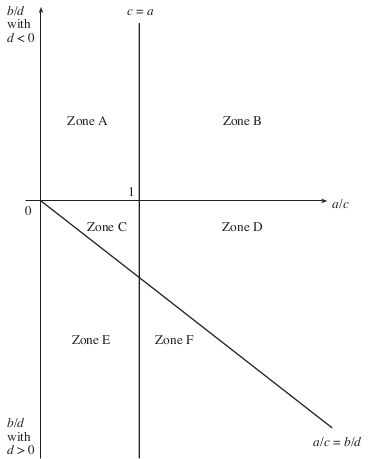
\includegraphics[scale=1]{market_plane_favereau.png}
		\fonte{\cite[p. 229]{favereau2002markets}}
	\end{figure}
	
	%To \citeonline{eloire2009reseaux}, the main goal of White's model is to show the structure of the market. The market plane shows six zones; four of them are zones that demarcate viable market, the other two, non-viable or unraveling. They can be described in a simplified way\footnote{A mathematical development of this plane is described in Appendix 1.} like this:
	
	Para \citeonline{eloire2009reseaux}, o principal objetivo do modelo de White é mostrar a estrutura do mercado. O plano do mercado mostra seis zonas; quatro delas são zonas que demarcam o mercado viável, as outras duas, o mercado não viável ou desvendado (\textit{unravelling}). Eles podem ser descritos de uma maneira simplificada da seguinte maneira:
	
	%Zone C is labelled \textbf{ordinary}. In this zone, revenues decrease to scale ($a/c < 1$) since cost increases with quality ($d > 0$). This is the `ordinary' that we think about quality. Also, returns are decreasing to quality to a more severe degree than to scale ($a/c > b/d$). Zones D and F are labelled \textbf{advanced}. In this zone higher quality is more expensive to produce ($d > 0$) and revenues increase to scale ($a/c > 1$). Zone A is labelled \textbf{paradox}. In this zone, in contrast with the ordinary thinking, higher quality is less costly to produce than lower quality ($d < 0$) although there are decreasing returns to scale ($a/c < 1$). B and E are non-viable market zones. 
	
	A zona C é chamada de \textit{ordinária}. Nessa zona, receitas diminuem com a escala ($a/c < 1$) visto que o custo aumenta com a qualidade ($d > 0$). Isto é o comum, o ``ordinário'', que pensamos sobre a qualidade. Além disso, os retornos diminuem com a qualidade em um grau mais severo do que com a escala ($a/c > b/d$). As zonas D e F são chamadas \textit{avançadas}. Nessa zona melhor qualidade é mais cara de ser produzida ($d > 0$) e as receitas aumentam com a escala ($a/c > 1$). A zona A é chamada \textit{paradoxo}. Nessa zona, em contraste com o pensamento ordinário, melhor qualidade é menos custosa de ser produzida do que pior qualidade ($d < 0$) embora os retornos diminuam com a escala ($a/c < 1$). B e E são zonas de mercado não viável.
	
	
	
	

	
	\subsection{Mensurações}
	
	\subsubsection{Como o modelo $W(y)$ tem sido mensurado}
	
	%In the $W(y)$ model, measurements are an issue to be solved in a creative way because White does not close the scope of the variables to be chosen. The review of two important studies gives us a basis to decide on this measurement issue.
	
	No modelo $W(y)$, as mensurações são uma questão a ser resolvida de uma maneira criativa devido ao fato de que White não fecha o escopo das possíveis variáveis a serem escolhidas para isso. A revisão de dois estudos importantes nos dá uma base para decidir sobre a questão da mensuração.
	
	%\citeonline{biencourt2002market} studied the theatrical institutions markets. They argue that the main advantage of White's model is related to the interdependence of the market structure and individual decisions through niches. This is particularly interesting to this specific case because
	
	\citeonline{biencourt2002market} estudou o mercado das instituições teatrais. Eles argumentam que a principal vantagem do modelo de White está relacionada à interdependência da estrutura do mercado e das decisões individuais através dos nichos. Isto é particularmente interessante para este caso específico porque
	
	\begin{citacao}
		Organizações teatrais baseiam a construção de seus nichos nas competências de seus times administrativo, técnico e artístico, nas experiências prévias do público e na política de elaboração dos programas que orienta as escolhas de repertório e diretores. O conceito de nicho é adequado à singularidade das performances. Sua qualidade é resultado de uma combinação da qualidade do trabalho individual dos atores e técnicos num projeto sob o controle do diretor\footnote{Theatrical organizations base their construction of niches on the competencies of their administrative, technical and artistic teams, the public's former experiences and the programming policy that orients choices of repertories and directors. The concept of a niche is suited to the uniqueness of performances. Their quality is the result of a combination of the quality of actors' and technicians' individual work on a project, under the control of the director.}. \cite[p. 255]{biencourt2002market}
	\end{citacao}
	
	
	%If we retake the functions of satisfaction (\ref{satisfaction}) and cost (\ref{cost}), the variables were chosen in this manner:
	
	Se retomarmos as funções de satisfação (\ref{satisfaction}) e custo (\ref{cost}), as variáveis foram escolhidas da seguinte maneira:
	
	\begin{itemize}
		\item \textbf{Volume de produção $Y$} -- estimado pelo número de performances listadas no relatório anual do teatro.
	\end{itemize}
	
	%The authors show that for \apudonline{throsby1993economics}{biencourt2002market} the number of tickets sold is a better suited indicator for $Y$. However, ``the determination of $S$ would then require one to know the degree of audience satisfaction after each performance, something that is impossible'' \cite[p. 264]{biencourt2002market}. The number of seats available for each performance would also have been a good indicator if the authors had access to this data.
	
	Os autores mostram que para \apudonline{throsby1993economics}{biencourt2002market} o número de ingressos vendidos é um indicador bem adequado para $Y$. Entretanto, ``a determinação de $S$ requereria que se conhecesse o grau de satisfação do público após cada performance, algo impossível\footnote{The determination of $S$ would then require one to know the degree of audience satisfaction after each performance, something that is impossible.}'' \cite[p. 264]{biencourt2002market}.  O número de assentos disponíveis para cada performance seria também um bom indicador se os autores tivessem acesso a esses dados.
	
	\begin{itemize}
		\item \textbf{Satisfação dos consumidores $S$} -- medida pelo número de visitantes pagantes à instituição.
	\end{itemize}
	
	%The authors justify this choice showing data from previous research on theatre audiences' habits and representations. Also, they divided the performances on four repertoire categories, namely, ``classical'', ``20th century'', ``contemporary French'' and ``contemporary foreign'' plays. They also make a correction for the repertory effect by ``multiplying the number of paying visitors observed  in each of the four categories by the average ratio $\bar{x}_i$ between the share of performances and that of the number of visitors in a given genre $i$ for all the institution markets'' \cite[p. 265]{biencourt2002market}. Let $\tilde{P}_i$ be the number of performances and $\tilde{V}_i$ be the number of paying visitors to all theatres in category $i$. The average can be defined by
	
	Os autores justificam essa escolha mostrando dados de pesquisas anteriores em hábitos do público do teatro e representações. Além disso, eles dividem as performances em quatro categorias de repertório, a saber, ``clássico'', ``século XX'', ``contemporâneo Francês'' e ``contemporâneo de outros países''. Eles também fazem uma correção para o efeito do repertório ``multiplicando o número de visitantes pagantes observados em cada uma das quatro categorias pela razão média $\bar{x}_i$ entre a proporção de performances e a proporção do número de visitantes em um dado gênero $i$ para todas as instituições do mercado\footnote{(\dots) Multiplying the number of paying visitors observed  in each of the four categories by the average ratio $\bar{x}_i$ between the share of performances and that of the number of visitors in a given genre $i$ for all the institution markets.}'' \cite[p. 265]{biencourt2002market}. Seja $\tilde{P}_i$ o número de performances e $\tilde{V}_i$ o número de visitantes pagantes para todos os teatros na categoria $i$. A média pode ser definida por
	
	\begin{equation}
	\label{repertory-effect-correction}
	\bar{x}_i = \frac{\tilde{P}_i / \sum_{i=1}^{4}\tilde{P}_i}{\tilde{V}_i / \sum_{i=1}^{4}\tilde{V}_i}	
	\end{equation}
	
	%If $v_i$ represents the number of paying visitors in category $i$ of repertoire, the public satisfaction can be estimated by
	
	Se $v_i$ representa o número de visitantes pagantes na categoria $i$ de repertório, a satisfação do público pode ser estimada por
	
	\begin{equation}
	\label{satisfaction-corrected}
	S = \sum_{i=1}^{4}\bar{x}_i v_i
	\end{equation}
	
	

	
	\begin{itemize}
		\item \textbf{O custo agregado $C$} -- esta variável foi obtida adicionando os custos artísticos do teatro (diferenciados aqui dos custos fixos).
		
		\item \textbf{escalar $r$} -- igual ao inverso do preço médio dos lugares $\bar{p}$ em todos os teatros.
		
		\item \textbf{escalar $q$} -- considerado igual a 1.
	\end{itemize}
	
	%Although White's model represents a big step in the construction of knowledge about the markets, it has an issue related to its very core, the quality ranking. To him, quality is given in a predetermined social space. In fact, \citeonline{favereau2002markets} states that to agree on price is not a big deal but to agree on quality is intrinsically a problem. We shall argue, however, that quality is not predefined but actors struggle and negotiate on a daily basis for its definition.
	
	Embora o modelo de White representa um grande passo na construção de conhecimento sobre os mercados, ele tem um problema relacionado com seu núcleo duro, o ranking de qualidade. Para ele, a qualidade é dada em um espaço social predeterminado. De fato, \citeonline{favereau2002markets} postula que concordar no preço não é uma grande coisa mas concordar na qualidade é intrinsecamente um problema. Argumentamos, entretanto, que a qualidade não é predefinida mas que os atores disputam e negociam diariamente pela sua definição.
	
	%According to \citeonline{eloire2009reseaux}, by embracing the annual publications previously mentioned, this industry has ``specific judgement devices on quality'' as \citeonline{karpik2009elements}  argues. This devices do not only help the coordination between offer and demand, but they also ``contribuent au classement des producteurs selon des critères de qualité collectivement définis et surtout acceptés, mais qui sont aussi des objets de lutte pour leur définition'' \cite[p. 494]{eloire2009reseaux}. In fact, \citeonline{eloire2009reseaux} states that the very existence of various guides is, by itself, an evidence of this symbolic struggles for the definition of quality, although in the ``high distinction'' the guides seem to converge.
	
	De acordo com \citeonline{eloire2009reseaux}, ao receber as publicações anuais previamente mencionadas, esse setor tem ``dispositivos de julgamento específicos para a qualidade'' como argumenta \citeonline{karpik2009elements}. Estes dispositivos não somente ajudam a coordenação entre oferta e demanda mas também ``contribuem à classificação dos produtores de acordo com os critérios de qualidade definidos coletivamente e sobretudo aceitos, mas que são também objetos de luta por definição\footnote{(\dots) Contribuent au classement des producteurs selon des critères de qualité collectivement définis et surtout acceptés, mais qui sont aussi des objets de lutte pour leur définition.}'' \cite[p. 494]{eloire2009reseaux}. De fato, \citeonline{eloire2009reseaux} postula que a própria existência de vários guias de qualidade é, em si, uma evidência dessa luta simbólica pela definição da qualidade, embora na ``alta distinção'' os guias tendam a convergir.
	
	%What if there are no guides or websites to testify on orchestra's quality and the critics in the main newspapers in town are nearly nonexistent? Well, this is the case in Belo Horizonte and it poses a quite of a challenge. All the cultural economics and singularities economics discussion on quality relies on the action of critics who are, per excellence, the ones who have the primacy of quality definition. In Belo Horizonte, orchestral performances almost never get a critic and there is not such a well structured platform for it as Rotten Tomatoes\footnote{\url{https://www.rottentomatoes.com}.} or \textit{Adoro Cinema}\footnote{A famous Brazilian movie critics website. Available in \url{http://www.adorocinema.com}.} for movies. If critics do not act much within the field of our study object, where does the quality definition come from?
	
	E se não houverem guias ou plataformas online especializadas para testificar da qualidade de uma orquestra e a presença de críticas nos jornais for ínfima? Este é o caso da cidade de Belo Horizonte, MG, e ele coloca um grande desafio à pesquisa. Toda a discussão da economia da cultura e da economia das singularidades sobre a qualidade repousa sobre uma ação dos críticos que são, por excelência, aqueles que possuem a primazia da definição da qualidade. Em Belo Horizonte as performances orquestrais quase nunca recebem uma crítica e não há uma plataforma bem estruturada para isso como o Rotten Tomatoes\footnote{\url{https://www.rottentomatoes.com}.} ou \textit{Adoro Cinema}\footnote{Um website brasileiro famoso de críticas de cinema. Disponível em \url{http://www.adorocinema.com}.}. Se as críticas não possuem grande atuação dentro do campo de nosso objeto de estudo, de onde vem a definição da qualidade?
	
	%\citeonline{biencourt2002market} present an interesting approach to the quality problem regarding theatres' market. We shall depart from their rationale to build the quality index $n$ we will use in this investigation.
	
	\citeonline{biencourt2002market} apresenta uma abordagem interessante para o problema da qualidade com relação ao mercado teatral. Partiremos de sua \textit{rationle} para construir o índice de qualidade $n$ que usaremos em nossa investigação.
	
	%To deal with quality index $N$, the authors elaborate a sophisticated construct to explain how various actors have a different influence on quality. To them,
	
	Para lidar com o índice de qualidade $N$, os autores elaboraram um construto sofisticado para explicar como vários atores tem diferentes influências sobre a qualidade. Para eles
	
	\begin{equation}
	\label{biencourt-quality}
	N_{l}^{b_l} = N_{1l}^{b_{1l}} N_{2l}^{b_{2l}} N_{3l}^{b_{3l}} N_{4l}^{b_{4l}} 
	\end{equation}
	
	%that is, the \textit{overall quality} $N$ in the year $l$ is constructed aggregating the judgements of \textit{drama critics} $N_1$, the judegements of \textit{programme planners} $N_2$, the judgement of the \textit{public authorities} $N_3$ and the influence of \textit{previous consumption} $N_4$. Now, each of these parts of the overall quality were measured in this manner:
	
	isto é, a \textit{qualidade geral} $N$ no ano $l$ é construída agregando as opiniões de \textit{críticos de teatro} $N_1$, as opiniões de \textit{planejadores de programas} $N_2$, a opinião de \textit{autoridades públicas} $N_3$ e a influência de \textit{consumo prévio} $N_4$. Cada uma das partes da qualidade geral foi mensurada da seguinte maneira:
	

	
	\begin{itemize}
		\item \textbf{Opiniões de críticos teatrais $N_1$} -- mensuradas registrando todas as críticas de apresentações agendadas nos teatros nos jornais \textit{Le Monde} e \textit{Libération} e na revista \textit{Télérama}, líderes de opinião entre os críticos teatrais.

		\item \textbf{Opiniões dos planejadores de programas $N_2$} -- a centralidade de grau de entrada normalizada do teatro; nesse caso, isso significa o número de performances de espetáculos produzidos por outras instituições teatrais agendadas pelo teatro divididas pela centralidade máxima da rede.
		
		\item \textbf{Opiniões de autoridades públicas $N_3$} -- mensurada pelo volume de subsídio do Estado. Para \citeonline[p. 267]{biencourt2002market}, ``essa escolha é justificada pelo peso do Estado que é maior do que o das autoridades locais no reconhecimento político da reputação de uma instituição artística\footnote{This choice is justified by the weight of the state, which is greater that that of local authorities in the political recognition of an institution's artistic reputation.}''.

		\item \textbf{Influência de consumos prévios $N_4$} -- mensurada pelo número de visitantes pagantes no período precedente.
	\end{itemize}
	
	%The overall quality perceived by the public is constructed by aggregating these four variables in the form of a Cobb-Douglas function (cf. equation \ref{biencourt-quality}). To measure the weight of each one of these variables on the overall quality, they estimated a linear model that had the number of paying visitors per performance as the dependent variable. Knowing that $r = 1/\bar{p}$ and taking into account equations (\ref{satisfaction}) and (\ref{biencourt-quality}), we can derive
	
	A qualidade geral percebida pela público é construída agregando essas quatro variáveis na forma de uma função Cobb-Douglas (cf. equação \ref{biencourt-quality}). Para medir o peso de cada uma das variáveis, eles estimaram um modelo linear que possuía o número de visitantes pagantes por performances como variável dependente. Sabendo que $r = 1/\bar{p}$ e levando em conta as equações (\ref{satisfaction}) e (\ref{biencourt-quality}), podemos derivar
	
	\begin{equation}
	\label{biencourt-derivation}
	[S\bar{p}/Y]_l = Y_{l}^{\hat{a}_l} N_{l}^{\hat{b}_l} \varepsilon_l = Y_{l}^{\hat{a}_l} N_{1l}^{\hat{b}_{1l}} N_{2l}^{\hat{b}_{2l}} N_{3l}^{\hat{b}_{3l}} N_{4l}^{\hat{b}_{4l}} \varepsilon_l
	\end{equation}
	
	%where $l$ is the year under investigation. This leads to the linear model
	onde $l$ é o ano sob investigação. Isso leva ao modelo linear
	
	\begin{equation}
	\label{regression}
	\log([S\bar{p}/Y]_l) = \hat{a}_l \log Y_l + \hat{b}_{1l} \log N_{1l} + \hat{b}_{2l} \log N_{2l} + \hat{b}_{3l} \log N_{3l} + \hat{b}_{4l} \log N_{4l} + \hat{\varepsilon}_l
	\end{equation}
	
	%From this, it is possible to deduce, without a constant,
	Disto é possível deduzir, sem a constante,
	
	\begin{equation}
	\label{N-com-pesos}
	\log N_l = \hat{b}_{1l} \log N_{1l} + \hat{b}_{2l} \log N_{2l} + \hat{b}_{3l} \log N_{3l} + \hat{b}_{4l} \log N_{4l} + e_l \hat{\varepsilon}_l
	\end{equation}
	
	%with $0 \le e_l \le 1$ assuming $\hat{b}_l = 1$.
	com $0 \le e_l \le 1$ assumindo $\hat{b}_l = 1$.
	
	%Then, the four elasticities exponents were deduced as solutions of a system of two equations to two unknowns. As the authors were studying two years seasons, by posing $\Delta = \log Y_l \cdot \log N_{l+1} - \log Y_{l+1} \cdot \log N_l$, they obtain:
	
	Então, os quatro expoentes de elasticidade foram deduzidos como soluções de um sistema de duas equações para dois desconhecidos. Como os autores estudaram duas temporadas, definindo $\Delta = \log Y_l \cdot \log N_{l+1} - \log Y_{l+1} \cdot \log N_l$, eles obtiveram:
	
	$$ a = \frac{ \log([S\bar{p}]_l) \cdot \log N_{l+1} - \log([S\bar{p}]_{l+1}) \cdot \log N_{l} }{\Delta} $$
	
	$$ b = \frac{ \log([S\bar{p}]_{l+1}) \cdot \log Y_{l} - \log([S\bar{p}]_{l}) \cdot \log Y_{l+1} }{\Delta} $$
	
	$$ c = \frac{ \log C_l \cdot \log N_{l+1} - \log C_{l+1} \cdot \log N_{l} }{\Delta} $$
	
	\begin{equation}
	\label{parameters}
	d = \frac{ \log C_l \cdot \log Y_{l+1} - \log C_{l+1} \cdot \log Y_{l} }{\Delta}
	\end{equation}
	
	

	
	% OBS: A partir da página 280, Éloire começar a falar dos niches de qualités e as variáveis que escolhe para medir cada parte do modelo.
	
	%On the other hand, \citeonline{eloire2009reseaux} chose a different set of variables to measure the inputs of the $W(y)$ model. In his PhD thesis, he studied the market of restaurants in Lille. He also uses the number of clients as an indicator to $y$ and observes the revenues (\textit{Chiffre d'affaires}) as well as uses the average ticket price for $W$. In order to investigate the market plane, \citeonline{eloire2009reseaux} mobilized the variables described in Table \ref{eloire-abcd}:
	
	Por outro lado, \citeonline{eloire2009reseaux} escolheu um set diferente de variáveis para medir os \textit{inputs} do modelo $W(y)$ Em sua tese de doutoramento, ele estudou o mercado dos restaurantes em Lille (França). Ele também usou o número de clientes como indicador de $y$ e observa as receitas (\textit{Chiffre d'affaires}) e o preço médio do ticket para $W$. Para investigar o plano do mercado, \citeonline{eloire2009reseaux} mobilizou as variáveis descritas na Tabela \ref{eloire-abcd}:
	
	\begin{table}[ht]
		\ibgetab{
			\centering
			\caption{Parâmetros de nichos de qualidade}
			\label{eloire-abcd}
		}
		{\begin{tabular}{c | p{5cm} p{5cm}}
				\hline
				& \textbf{Volume}  & \textbf{Qualidade} \\
				\hline
				\textbf{Satisfação}  & \textbf{a} = Número médio de clientes por serviço & \textbf{b} = Valor médio do ticket + Nota da qualidade \\
				\textbf{Custo} & \textbf{c} = Assalariados / \textit{Couverts} * Serviços & \textbf{d} = Razão de disponoibilidade de assalariados / clientes \\
				\hline
			\end{tabular}
		}
		{\fonte{\citeonline[p. 289]{eloire2009reseaux}}}
	\end{table}




	% This here is on page 290!!!
	%Éloire argues that quality is a social construction build between the offer from structured producers and an aggregated demand. In the restaurants case, it also depends on the ``cuisine'' style which is very difficult to measure. However, this culinary scale is closely correlated with simple economic statistics: price, availability ratio in a way that the higher the prices and the ratio, the more ``fancy'' is the restaurant. Therefore, he considers the quality cost (\textbf{d} parameter) is related to the availability ratio, that is the amount of personnel that a restaurant hires over the number of clients it intends to serve. Clients satisfaction (\textbf{b} parameter) can be represented by the average ticket value.
	
	Éloire argumenta que a qualidade é uma construção social feita entre a oferta de produtores estruturados e a demanda agregada. No caso dos restaurantes, isso também depende do estilo de \textit{cuisine} o qual é bastante difícil de mensurar. Entretanto, essa escala culinária está fortemente correlacionada com estatísticas econômicas simples: preço, taxa de de disponibilidade de modo que quanto maior os preços e a taxa, mais ``\textit{chic}'' é o restaurante. Portanto, ele considera que o custo de qualidade (o parâmetro \textbf{d}) está relacionado com a razão de disponibilidade, isto é, a quantidade de pessoal que o restaurante contrata sobre o número de clientes que ele intenciona servir. A satisfação da clientela (o parâmetro \textit{b}) pode ser representado pelo valor médio do ticket.
	
	% PAGE 290
	%The author recognizes that the a restaurant's capacity is correlated to the volume of personnel. So, the volume costs (\textbf{c} parameter) are measured to the number of salaried employees divided by the (potential) number of cutlery multiplied by the number of services. Also, he acknowledges that a main strategy of the restaurants is related to the amount of time/time of the day that it stays open. Some restaurants can function 24/7, some only at lunch, some only at night,  and this implicates requires cost, personnel, logistics, etc. This is expressed on the \textbf{c} parameter calculus. The satisfaction at volume (\textbf{a} parameter) is measured by the average number of clients per service. This is derived of the restaurant's ``filling rate''. The higher this rate, the more we can infer that his decisions regarding volume costs are validated by the clients. On the other hand, the lower this rate, the more the volume costs can be seen as ``disproportional'' by the clients \cite{eloire2009reseaux}.
	
	O autor reconhece que a capacidade de um restaurante está correlacionada com o volume de pessoal. Portanto, o volume de custos (o parâmetro \textbf{c}) é medido pelo número de empregados assalariados dividido pelo número (potencial) de talheres multiplicado pelo número de serviços. Ainda, ele percebe que a principal estratégia dos restaurantes está relacionada com a quantidade de time/a hora do dia em que ele permanece aberto. Alguns restaurantes podem funcionar 24hs, alguns apenas no horário de almoço, outros apenas à noite, e isso implica custos, pessoal, logística, etc. Isto é expresso no cálculo do parâmetro \textbf{c}. A satisfação quanto ao volume (o parâmetro \textbf{a}) é medida pelo número médio de clientes por serviço. Isto é derivado da ``taxa de lotação'' do restaurante. Quanto maior a taxa, mais é possível inferir que suas decisões quanto aos custos de volume são validadas pelos clientes. Por outro lado, quanto menor a taxa mais os custos de volume podem ser vistos como ``desproporcionais'' pelos clientes \cite{eloire2009reseaux}.
	
	%The quality note pointed by the author in table \ref{eloire-abcd} is built aggregating the notes of five international restaurant guides, all of them well known and recognized in the profession, namely, ``Le Guide Michelin France'', ``Le Bottin Gourmand'', the ``GaultMillau'', the ``Champérard'' and ``Le Pudlo France''. The aggregation of these guides scoring was obtained through a specialized website\footnote{\url{http://restaurant-hitlisten.de/france/bewertung.htm}}.
	
	A qualidade da nota apontada pelo autor na tabela \ref{eloire-abcd} é construída agregando as notas de cinco guias internacionais de restaurantes, todos muito bem conhecidos e reconhecidos na meio profissional, a saber, ``Le Guide Michelin France'', ``Le Bottin Gourmand'', o ``GaultMillau'', o ``Champérard'' e ``Le Pudlo France''. A agregação das notas desses guias foi obtida através de um site especializado\footnote{\url{http://restaurant-hitlisten.de/france/bewertung.htm}}.
	
	
	


	\subsection{Nossa proposta de mensuração}
	
	
	Retomemos as duas principais equações do modelo $W(y)$. Primeiro a equação de custo (\ref{cost}):
	$$C(y, n) = q \cdot y^c \cdot n^d$$
	e a equação de satisfação (\ref{satisfaction}):
	$$S(y, n) = r \cdot y^a \cdot n^b$$
	
	Para os propósitos desta investigação os parâmetros serão mensurados da seguinte maneira:
	
	\begin{itemize}
		\item A constante $q = 1$;
		\item A constante $r =$ o inverso do preço médio do ingreso nas performances da temporada, isto é, $1/\bar{p}$;
		\item O custo agregado $C$ será obtido pelos custos artísticos da orquestra;
		\item A satisfação do público $S$ será estimada pela razão entre o número de indivíduos pagantes no público sobre o número de assentos;
		\item O volume de produção $y$ será estimado pelo número de assentos disponíveis para cada performance\footnote{Caso não tenhamos acesso a esse dado, $y$ será estimado pelo número total de performances na temporada.};
		\item O índice de qualidade $n$ será estimado agregando o preço do ticket, o orçamento total, ``proximidade com o Estado'' e a percepção dos músicos;
		\item ``A proximidade com o Estado'' será mensurada pelo número de contratos assinados e o financiamento total proveniente do Estado.
	\end{itemize}
	
	
	%The elasticities $a$ and $b$, related to the Satisfaction equation, can be obtained as solutions of a system of two equations to two unknowns as proposed by \citeonline{biencourt2002market}. Trying to measure any of these variables would violate the assumption that cultural goods are not rivals in consumption.
	
	As elasticidades $a$ e $b$, relacionadas à equação de satisfação, podem ser obtidas como soluções de um sistema de duas equações para dois desconhecidos como proposto por \citeonline{biencourt2002market}. Tentar medir algumas dessas variáveis violaria o pressuposto de que bens culturais não são rivais no consumo.
	
	%The elasticities $c$ and $d$, on the other hand, can be measured in the following way:
	% ELABORATE! ELABORATE! ELABORATE! ELABORATE! ELABORATE!
	
	As elasticidades $c$ e $d$, por outro lado, podem ser mensuradas da seguinte maneira:
	
	\begin{itemize}
		\item $c =$ o número de empregados assalariados  $/$ número de performances;
		\item $d =$ orçamento total $/$ número de performances.
	\end{itemize}
	
	A tabela \ref{measurements-wy} sintetiza as variáveis escolhidas como indicadores para medir os \textit{inputs} do modelo $W(y)$.
	
	\begin{table}
		\ibgetab{
			\caption{Indicadores propostos - modelo $W(y)$}
			\label{measurements-wy}
		}
		{\begin{tabular}{|c|c|}
				
				\hline
				\textbf{Conceito} & \textbf{Indicador} \\
				\hline
				A constante \textbf{q} & 1 \\
				\hline
				A constante \textbf{r} &  $1/\bar{p}$ \\
				\hline
				Custo agregado \textbf{C} & Despesas artísticas \\
				\hline
				Satisfação \textbf{S} & Indivíduos pagantes / assentos à disposição \\
				\hline
				Volume de produção \textbf{y} & Assentos disponíveis (ou número de performances) \\
				\hline
				Índice de qualidade \textbf{N} & Preço do ingresso, \\
				& Orçamento total, \\
				& ``Proximididade com o Estado'', \\
				& Precepção dos músicos. \\
				\hline
				``Proximidade com o Estado'' & Número de contratos assinados, \\
				& Financiamento total do Estado. \\
				\hline
				A elasticidade \textbf{c} & Número de empregados / número de performances \\
				\hline
				A elasticidade \textbf{d} & Orçamento total / número de performances\\
				\hline
			\end{tabular}
		}
		{\fonte{Elaborado pelo autor.}}
	\end{table}

	



	\section{A arquitetura dos mercados}

	Neil \citeonline{fligstein2002architecture} traça uma teorização sobre a emergência e funcionamento dos mercados ligeiramente diferente da que vimos em White. Fligstein também leva em conta uma estrutura relacional onde firmas interagem entre si e com o comprador generalizado visando a estabilização do mercado (e consequente subsistência de todos). A grande diferença fica por conta da participação do Estado. Enquanto White não tece grandes considerações acerca do papel estatal na emergência e funcionamento dos mercados de produção, Fligstein elabora seu esquema teórico identificando a estrutura do Estado como central para o desenvolvimento dos mercados. Por que Estados? - pergunta Fligstein. O próprio autor responde que ``À medida que a possibilidade de padrões de interação complexos na esfera da troca econômica se expandem, os atores se mostraram incapazes de prover regras para si mesmos\footnote{As the possibility for complex patterns of interaction in the sphere of economic exchange has expanded, actors have proven incapable of providing rules for themselves.}'' \cite[p. 27-8]{fligstein2002architecture} e, portanto, recorrem ao Estado como provedor de regras para que o jogo econômico funcione de maneira justa.

	\citeonline{fligstein2002architecture} concebe os mercados como ``campos'', arenas sociais onde vendedores e compradores se encontram. Essas arenas obedecem a quatro tipos puros de regras para a produção e reprodução de sua estrutura, quais sejam:

	\begin{enumerate}
		\item direitos de propriedade;
		\item estruturas de governança;
		\item regras de troca e
		\item concepções de controle.
	\end{enumerate}

	Estas diferentes formas de regulação são inclusivas; o nível posterior necessariamente pressupõe o anterior. Do primeiro ao último há um maior grau de generalidade.

	Direitos de propriedade são, segundo o autor, regras que definem quem possui diretos sobre os retornos financeiros das firmas. Formas comuns de direito de propriedade são patentes e credenciais. Sua constituição não é, necessariamente, o desfecho de um processo eficiente mas um contínuo e contestável processo político \cite{fligstein2002architecture}.

	Essa regras configuram condição \textit{sine qua non} de existência de mercados uma vez que definem as relações entre aqueles que detém posse de algum bem e os demais estabilizando o mercado. ``Os direitos de propriedade funcionam, portanto, para produzir duas formas de estabilidade: a definição de relações de poder entre constituintes dentro e fora das firmas e sinalizar a outros quem essas firmas são\footnote{Property rights thus function to produce two forms of stability: defining the power relationships between constituencies in and around firms, and signaling to other firms who firms are.}'' \cite[p. 34]{fligstein2002architecture}.

	Estruturas de governança são estruturas de regras gerais ao nível da sociedade que definem relações competitivas e cooperativas entre firmas além de sua organização interna. Essas regras definem formas legais e ilegais de controle da competição no espaço mercantil. Elas podem aparecer na forma de leis (e.g., leis antitrustes) ou normas sociais muito embora assumam grande variação entre diferentes sociedades. Cabe ressaltar que a organização interna de uma firma também se dá como resposta a formas legais ou ilegais de competição no mercado. Firmas podem se integrar tanto verticalmente, como forma de assegurar seus insumos necessários, quanto horizontalmente, comprando ações visando produzir um ordenamento estável no mercado ou diversificando sua carta de produtos visando proteção contra os ``caprichos de produtos específicos'' \cite[p. 34]{fligstein2002architecture}. A formação de parcerias estáveis e de longo prazo também configuram respostas à competição.

	As regras de troca definem quem pode se engajar em transações comerciais com quem bem como suas condições. As regras abrangem pesos, padrões comuns, fretagem, cobrança, seguro, trocas financeiras e a firma de contratos. ``As regras de troca ajudam a estabilizar os mercados assegurando que as trocas ocorram sob condições que se aplicam a todos\footnote{Rules of exchange help stabilize markets by ensuring that exchanges occur under conditions that apply to everyone.}'' \cite[p. 35]{fligstein2002architecture}. Alguns dos tratados comerciais internacionais mais recentes como o GATT (\textit{General Agreement of Tariffs and Trade}) focam na harmonização das regras de troca.

	``Concepções de controle refletem acordos específicos de mercado entre atores em firmas sobre princípios de organização interna (\dots), táticas de competição ou cooperação (\dots), e a hierarquia ou o ordenamento de status das firmas num dado mercado\footnote{Conceptions of control reflect market-specific agreements between actors in firms on principles of internal organization (\dots), tactics for competition or cooperation (\dots), and the hierarchy or status ordering of firms in a given market.}'' \cite[p. 35]{fligstein2002architecture}. São, em sua essência, produtos histórico-culturais. São históricos à medida que se restringem ao contexto histórico de um determinado setor em uma determinada sociedade e são culturais pois formam um arcabouço de entendimentos e práticas vigentes num dado mercado. Para \citeonline{fligstein2002architecture}

	\begin{citacao}
		Um mercado estável é um campo social no qual a concepção de controle define as relações sociais entre firmas vendedoras incumbentes e desafiantes de modo que as incumbentes reprodruzem essas relações de tempos em tempos. O propósito da ação em um dado mercado é criar e manter mundos estáveis dentro das firmas e entre elas que permita a sobrevivência de firmas dominantes\footnote{A stable market is a social field in which a conception of control defines the social relations between incumbent and challenger seller firms such that the incumbent firms reproduce those relations on a period-to-period basis. The purpose of action in a given market is to create and maintain stable worlds within and across firms that allow dominant seller firms to survive.}. \cite[p. 35]{fligstein2002architecture}
	\end{citacao}

	As concepções de controle evidenciam também, como podemos notar, um elemento político dos mercados no que toca à manutenção do ordenamento hierárquico vigente, sua reprodução e sua manifestação no processo de definição de padrões de qualidade e certificação. Dito de outra forma, as concepções de controle colocam perguntas como ``quem controla a entrada e saída de um sistema concorrencial?'' ``Como os desafiadores e os dominantes entram em relação?'' ``Quem consegue impor a pauta de qualidade num setor industrial, por exemplo, um \textit{standard} ISO ou um sistema de certificação do que é um produto orgânico no mercado de alimentos?''

	Para Fligstein, a entrada de países em sistemas capitalistas ``empurra'' os Estados a uma posição regulatória com relação aos quatro tipos acima mencionados. No exercício regulatório, os Estados produzem normativas culturais que determinam o processo de estruturação da ação econômica. Esse exercício é contínuo. Constantemente os Estados lidam com situações de crise e com o \textit{lobby} das empresas clamando por intervenção estatal. Os rumos que os mercados tomam estão diretamente relacionados a dois fatores: (1) a capacidade de intervenção, regulação e mediação do Estado e (2) o poder de organizações privadas para influenciar os termos de intervenção.

	O Estado tem ainda um papel fundamental no financiamento da inovação. Segundo \citeonline{fligstein2002architecture}

	\begin{citacao}
		Os governos nas sociedades industriais tem um papel importante quanto ao investimento e mediação da luta de classe. As ações dos empresários e empreendedores são enquadradas em torno dessas formas de estabilidade. Eles podem criar novos setores usando a ajuda do governo para investir em tecnologias arriscadas. Eles podem diversificar os riscos em suas firmas para produzir identidades estáveis para as firmas\footnote{Governments in industrial societies play a role in investment and mediating the class struggle as well. The actions of managers and entrepreneurs are framed around these forms of stability. They can create new industries using government support to invest in uncertain technologies. They can diversify their risks in their firms to produce stable identities for firms.}. \cite[p. 62]{fligstein2002architecture}
	\end{citacao}

	Para esse autor, seria muito difícil imaginar a existência de um mercado sem o aparato estatal cuidando de seu regulamento e estabilização. Isso, entretanto, não implica que a atuação estatal seja neutra mas ela reproduz o controle de grupos sociais dominantes os quais mantém uma relação próxima do Estado e tem primazia nos pedidos de intervenção em épocas de crise. Sem as regras e acordos geridos pelo Estado, não haveria uma organização-social mínima para que produtores possam arriscar com novos produtos fazendo emergir novos mercados.

	Para Fligstein, num mercado o preço é um indicador confiável de qualidade. As empresas se veem impelidas pela competição de preços a diferenciar seus produtos formando nichos como forma de proteção contra a instabilidade. A diversificação da carta de produtos é também uma estratégia dominante para a diminuição de riscos. ``Uma firma pode produzir produtos múltiplos que reduzem sua dependência em um produto específico e, portanto, aumenta suas chances de sobrevivência\footnote{A firm can produce multiple products that reduce their dependence on any one product and, hence, increase the likelihood that the firm will survive.}'' \apud[p. 74]{kay1997pattern}{fligstein2002architecture}.

	\citeonline[p. 81]{fligstein2002architecture} postula ainda que ``em mercados com concepções de controle estáveis, os participantes amplamente concordam com a concepção de controle, com a hierarquia de status e as estratégias que ela implica\footnote{In markets with stable conceptions of control, market participants widely agree on the conception of control and the status hierarchies and strategies it implies.}''. Uma vez estabilizado, o mercado é compreendido tanto por firmas estabelecidas como ``desafiantes'' em sua estrutura de poder. Essa estrutura permite a avaliação da ação e das estratégias das firmas por qualquer observador e, consequentemente, sua ação orientada sobre essas estratégias. Aqui, estamos muito próximos ao que White chama de ``disciplina'' do mercado.

	As crises nos mercados são percebidas quando firmas estabelecidas começam a falir. Isso pode ser causado por três eventos: (1) queda na demanda pelo produto o que pode ser proveniente de más condições econômicas ou mudanças nas preferências dos compradores, (2) a entrada de uma nova firma no mercado distorcendo a concepção de controle vigente e forçando a reorganização do mercado ou (3) o Estado pode, intencionalmente ou não, mudar as regras vigentes e desestabilizar o mercado.

	É curioso notar que enquanto para Fligstein o Estado tem um papel preponderante na estrutura de mercado, para White o Estado não conta com a mesma importância. Sua teoria é construída nas relações entre firmas, em sua capacidade de percepção do tecido relacional que compõe a estrutura do mercado e na diferenciação de hierarquias por qualidade. Ambos os autores também divergem quanto à postura de cada firma em relação a seu posicionamento no mercado. Para White, a busca pelo posicionamento ótimo advém da observação dos pares engajamentos/retornos. A hierarquização das firmas (e consequente estabilização do mercado numa interface inteligível por todos) se dá por meio da qualidade percebida. Já para Fligstein, a busca pelo posicionamento se dá através de estratégias de proteção contra a concorrência dos preços (construção de nichos de mercado), da diversificação da carta de produtos oferecidos num ambiente que visa a estabilidade onde a figura central de controle é o Estado.

	A abordagem de Fligstein, como vimos, dá um papel central ao Estado como articulador, regulador e estabilizador do mercado. Sem ele, a estrutura não teria condições para fazer emergir uma normativa compartilhada que servisse como regime de controle, solo sólido para orientação da ação econômica e elaboração de estratégias de atuação. Estamos falando do clássico problema da ação coletiva; ela se preocupa em barrar a atuação de ``caronas'' e alocar de forma equânime custos de produção de bens públicos. Como podemos pensar num mercado, uma estrutura concorrencial por excelência, como uma ação coletiva? Ocorre cooperação? De fato, para que o mercado se estabilize e haja distribuição igualitária de oportunidades e acesso ao mercado tanto por firmas dominantes quanto desafiantes, em alguma medida  elas acabam cooperando mesmo que essa cooperação ocorra em um nível supraintencional. Isso se assemelha ao famoso conceito da ``mão invisível'' de Adam Smith. O trabalho do sociólogo seria, portanto, torná-la visível.

	%Resta ainda uma investigação mais profunda sobre o processo de atuação das firmas no dia a dia engajando-se em movimentos ao mesmo tempo de competição e cooperação. O conceito de isomorfismos organizacionais parecem lançar uma boa luz sobre esses processos. Vejamo-los mais detidamente.



	
	\section{A busca de nichos como processo social regulatório}

	Para \citeonline{lazega2009theorie}, a busca das firmas pela estabilização de um mercado passa por uma noção de qualidade construída coletivamente a partir das relações tecidas pelas firmas. Em sua atuação, as firmas se engajam em processos ao mesmo tempo de competição e cooperação -- o que ficou conhecido na sociologia das organizações como \textit{coopetition}. As organizações não conduzem seus negócios de maneira isolada mas são necessariamente dependentes de alguns recursos que as forçam a tecer laços de cooperação com outras organizações. Essas relações podem se manifestar na forma de um quadro jurídico e social mais ou menos definido. Segundo o autor, ``esses recursos interorganizacionais trocados através de laços multiplexos, podendo consistir de aprendizado, bens ou serviços, não são forçosamente de natureza monetária ou puramente funcional\footnote{Ces resources interorganisationnelles, échangés à travers des liens multiplexes, et pouvant consister en de l'apprentissage, des biens, des services, ne sont pas forcément de nature monétaire ou purement fonctionnelle.}'' \cite[p. 568]{lazega2009theorie}.

	Em sua atuação, o empreendedor busca a estruturação de seu contexto de interações e de negócios visando a sua própria segurança no mercado e a de seus investimentos relacionais. Esse processo, que possui uma forte capacidade de politização, leva o empreendedor a uma autorestrição contextual quanto à seleção de seus parceiros comerciais. Segundo o autor

	\begin{citacao}
	A troca social conduz o empreendedor a uma forma de autodisciplina social que se apoia de fato sobre uma endogeneização (\dots) das estruturas relacionais. Essa endogeneização toma a forma de manutenção ou construção de nichos sociais bem como de entrada na concorrência por status social\footnote{L'échange social conduit ainsi l'entrepreneur à une forme d'autodiscipline sociale qui s'appuie en fait sur une endogénéisation (\dots) des structures relationnelles. Cette endogénéisation prend la forme de l'entretien ou de la construction de niches sociales ainsi que celle d'une entrée dans la concurrence de statut social.}. \cite[p. 572]{lazega2009theorie}
	\end{citacao}

	A busca por nichos sociais, desse modo, é um primeiro meio de mobilização de uma estrutura de oportunidades. O nicho social, portanto, pode ser definido como o ``subconjunto de colegas-concorrentes com os quais se tem relações especialmente densas, multifuncionais, duráveis e ligadas, direta ou indiretamente, a suas atividades de produção\footnote{(\dots) le sous-ensemble de collègues-concurrents avec lesquels il/elle a des relations spécialement denses, multifonctionnelles, durables et liées, directement ou indirectement, à ses activités de production.}'' \cite[p. 575]{lazega2009theorie}.

	Na estruturação do tecido social que compõe o mercado processos sociais se articulam com disciplinas sociais emergentes proporcionando uma estrutura cognitiva pela qual pode-se orientar a ação econômica. Nessa articulação, quatro processos sociais se engajam com disciplinas:

	\begin{enumerate}
		\item Apredizado coletivo;
		\item Fenômenos de solidariedade;
		\item Controle social e
		\item Regulação e institucionalização.
	\end{enumerate}

	De maneira bastante breve, o aprendizado coletivo ou aprendizado organizacional ocorre a partir de fluxos de informações, recursos (humanos ou materiais) e através de trocas de conhecimento tácito. Fenômenos de solidariedade podem ocorrer na presença de ameaças ou instabilidade no mercado. Acordos comerciais, coletivos, associações entre empresas que, embora concorrentes, cooperam, emergem como estratégia de conquista de espaço no campo social. O controle social é facilitado pelos nichos sociais e pelo reconhecimento de uma estrutura de status entre organizações. Por fim, processos de regulação e institucionalização consistem da redefinição das regras do jogo. Nesse processo, organizações competem e cooperam para estabelecer uma linguagem de referência, um corpo normativo comum.
	
	%Our research aims to investigate a social regulatory process par excellence: the construction of the quality standard. As we saw, the quality index is the main gear that makes the orchestral music market engine run. The emergence of quality is a regulatory process that comes out of a struggle between the various actors involved in the market (musicians, public, critics, the State). The outcome would not necessarily be defined in terms of which actor is the most powerful, as conventional sociological theory would state, but it will emerge as a construct from complex interactions of \textit{coopetition} movements of the actors.
	
	Nossa pesquisa está interessada em investigar um processo social regulatório por excelência: a construção do padrão de qualidade. Como vimos, o índice de qualidade é a principal engrenagem que faz o motor do mercado da música de concerto funcionar. A emergência de qualidade é um processo regulatório que emerge de uma disputa entre vários atores envolvidos no mercado (músicos, público, crítica, o Estado). O resultado não seria necessariamente definido em termos de investigar qual ator detém mais poder, como a teoria sociológica convencional colocaria, mas emerge como um construto de interações complexas de movimentos de \textit{coopetição} entre os atores.
	
	\section{Isomorfismos normativos}

	Ao se debruçar sobre o mesmo fenômeno, a estruturação do campo de um mercado, \citeonline{dimaggio1983iron} mobilizam o conceito de isomorfismo para dar conta dos processos de competição-cooperação nos quais as organizações se engajam. Esses autores partem da seguinte pergunta: Por que as organizações são tão parecidas? Embora a pergunta pareça trivial, ela não é de nenhum modo intuitiva. A questão está em diálogo com um diagnóstico amplo da sociologia weberiana em relação à crescente racionalização do mundo industrial. Ora, se nos mercados a ação racional é concorrencial, esperaríamos que houvesse maior diversificação das formas organizacionais, cada uma buscando meios diferentes de subsistência. Não é o que os autores percebem ao postular a questão supracitada. %verificar isso com o Silvio

	Uma vez que organizações diversas se engajam numa mesma linha de mercado formando um estrutura (um campo), os processos que levam à similaridade começam a emergir com robustez.

	De que falamos, entretanto, quando falamos em isomorfismos? \citeonline[p. 149]{dimaggio1983iron} definem o termo como ``um processo de controle que força uma unidade na população a assemelhar-se a outras unidades que encaram o mesmo conjunto de condições ambientais\footnote{(\dots) a constraining process that forces one unit in a population to resemble other units that face the same set of environmental conditions.}''.

	\citeonline{dimaggio1983iron} citam três mecanismos de isomorfismos: (1) Isomorfismos coercitivos, (2) isomorfismos miméticos e (3) isomorfismos normativos. Os isomorfismos coercitivos resultam de pressões formais e informais sobre as empresas. Expectativas relacionadas a normas sociais ou a padrões culturais também são gatilhos para esse mecanismo. Por vezes, o Estado também pode impulsionar esse tipo de isomorfismo estabelecendo novas políticas de controle sobre o funcionamento dos mercados (como padrões para controle de resíduos ou emissão de gases, por exemplo).

	Os isomorfismos miméticos surgem em resposta à incerteza do mercado. Em face a um cenário de incertezas, uma firma pode imitar o modelo de uma outra que seja bem sucedida no mercado. Os isomorfismos normativos advém de normativas e tradições bem como, principalmente, da crescente profissionalização. Um coletivo profissional pode, por exemplo, empreender esforços para definir condições e métodos de seu estrato profissional, estabelecer critérios de controle ou estabelecer uma base cognitiva e legitimação para a autonomia ocupacional.

	Os processos de isomorfismo lançam luz sobre o comportamento observado nas orquestras em geral (embora seja difícil explicar como os três tipo puros operam simultaneamente). Já argumentamos que todos os grupos orquestrais estão comprometidos com um padrão de qualidade comum pelo qual são posicionados numa hierarquia percebida na estrutura do mercado tanto por eles mesmos quanto pelo público. Tentativas de uma orquestra de recolocação dentro da escala hierárquica, por exemplo, podem ser empreendidas através de sua reformulação interna objetivando aproximar-se das características da organização dominante naquele cenário. Para isso, a orquestra lançará mão ainda de mecanismos de cooperação (com as diversas identidades que integram o mercado) onde aprenderá processos, lançará mão de recursos, etc.

	Até aqui, os diversos \textit{frameworks} teóricos parecem convergir de maneira complementar no que toca a análise do mercado da música orquestral. Apresentaremos, a seguir, o modelo de análise que norteará esta investigação.




	\chapter{A abordagem multinível}
	
	
	 %\citeonline{lazega2016synchronization}\footnote{\citeonline{lazega2016synchronization} gives a theoretical introduction to multilevel networks. For a technical introduction as well as a reconstruction of the operationalization of the concept, see \citeonline{snijders2016multiple}.} states that a sociological tradition whose  origins are attributed to Max Weber develops itself to point out a kind of society that \apudonline{perrow1991society}{lazega2016synchronization} calls ``organizational'' and \apudonline{breiger1974duality}{lazega2016synchronization} calls ``dual''. Both concepts point to ``two levels of collective agency that co-constitute each other: an inter-individual level and an inter-organizational level'' \cite[p. 48]{lazega2016synchronization} between all kinds of collective entities. Individuals are distributed within a social structure where they have ties which each other, where they are affiliated to organizations and where those organizations also relate and build ties to each other. This makes the actors look at the world in a multilevel perspective and be aware of the importance of accounting for people's belongings to collectivities and the relations between these collectivities in a higher order to rationalize their actions in terms of control and efficiency. To \citeonline[p. 48]{lazega2016synchronization}, ``without this multilevel coordination (\dots), neither individuals nor organizations can access or mobilize on their own all the resources that are needed to produce, compete and survive''.
	 
	 \citeonline{lazega2016synchronization}\footnote{\citeonline{lazega2016synchronization} apresenta uma introdução teórica das redes multinível. Para uma introdução técnica bem como uma reconstrução da operacionalização do conceito, cf. \citeonline{snijders2016multiple}.} postula que uma tradição sociológica cujas origens remetem a Max Weber se desenvolve apontando um tipo de sociedade a qual \apudonline{perrow1991society}{lazega2016synchronization} chama de ``organizacional'' e \apudonline{breiger1974duality}{lazega2016synchronization} chama de ``dual''. Ambos os conceitos apontam para ``dois níveis de agência coletiva que co-constituem um ao outro: um nível interindividual e um nível interorganizacional\footnote{two levels of collective agency that co-constitute each other: an inter-individual level and an inter-organizational level}'' \cite[p. 48]{lazega2016synchronization} entre todos os tipos de entidades coletivas. Indivíduos são distribuídos dentro de uma estrutura social onde eles possuem laços uns com os outros, onde são afiliados a organizações e onde essas organizações também se relacionam e constroem laços umas com as outras. Isto faz os atores olharem para o mundo de uma perspectiva multinível e estarem apercebidos da importância de levar em conta os pertencimentos das pessoas a coletividades e as relações entre essas coletividades num plano mais alto para racionalizar suas ações em termos de controle e eficiência. Para \citeonline[p. 48]{lazega2016synchronization}, ``sem essa coordenação multinível (\dots), nem indivíduos nem organizações podem acessar ou mobilizar sozinhos todos os recursos necessários para produzir, competir e sobreviver\footnote{Without this multilevel coordination (\dots), neither individuals nor organizations can access or mobilize on their own all the resources that are needed to produce, compete and survive.}''.
	
	%Interpersonal interdependencies are formed out of cowork, advice, friendship and other kind of relations built within or across organizations. The rules that organize social exchange are also part of these interdependencies. Inter-organizational interdependencies, on the other hand, are created mostly by contractual agreements between entities where contributions, rights and responsibilities are defined in the pursue of a common goal. It also depends on institutions that guarantee its credibility. It is important to notice that the relations are much less personalized in the organizational level. ``Resources, commitments and rules are different in nature from those characterizing the inter-individual level of agency'' \cite[p. 49]{lazega2016synchronization}. The links between those two levels are created by member affiliations on one level to the other (typically individuals in organizations). These approach is called `linked design' \cite{lazega2008catching}. 
	
	Dependências interpessoais são formadas de trabalho conjunto, aconselhamento, amizade e outros tipos de relações construídas dentro ou entre as organizações. As regras que organizam a troca social são também parte dessas interdependências. Interdependências organizacionais, por outro lado, são criadas principalmente por acordos contratuais entre entidades onde contribuições, direitos e responsabilidades são definidas na busca de um objetivo comum. Elas também dependem das instituições que garantem sua credibilidade. É importante notar que as relações são muito menos pessoais no nível das organizações. ``Recursos, compromissos e regras são diferentes em sua natureza daquelas que caracterizam o nível de agência interindividual\footnote{Resources, commitments and rules are different in nature from those characterizing the inter-individual level of agency.}'' \cite[p. 49]{lazega2016synchronization}. As ligações entre esses dois níveis são criadas por afiliações de membros de um nível a outro (tipicamente indivíduos a organizações). Essa abordagem é chamada de ``\textit{linked design}'' \cite{lazega2008catching}.
	
	%When accounting for the interdependencies of both levels horizontally(within each level) and vertically (affiliations between levels), we can observe overlap and complementarity from which arise complex combinations of the various interests at stake. Also, actors are displayed in a stratified structure where status hierarchy is perceived not only regarding their individual assets, but also their organizations'. There can be ``big fish in big pond'', ``small fish in big pond'', and so on. \cite{lazega2008catching}.
	
	Quando levamos em conta as interdependências de ambos os níveis horizontalmente (dentro de cada nível) e verticalmente (as afiliações entre os níveis), podemos observar sobreposições e complementaridade das quais emergem combinações complexas de vários interesses em disputa. Além disso, atores são dispostos em uma estrutura estratificada onde a hierarquia de status é percebida não somente com relação aos recursos individuais, mas também com relação aos recursos organizacionais. Podem haver ``peixes grandes em aquários grandes'', ``peixes pequenos em aquários grandes'', e assim por diante \cite{lazega2008catching}.



	\citeonline{brailly2016market} estudam um mercado internacional entre organizações. De acordo com os autores, por trás das relações interorganizacionais há sempre laços entre indivíduos. Algumas organizações precisam de encontros interpessoais para iniciarem ações conjuntas ou parcerias. À medida que essas parcerias se repetem a relação se torna cada vez mais interorganizacional e cada vez menos interpessoal caminhando em direção a prescindir de encontros entre membros específicos. Os autores argumentam que, para um melhor entendimento dos fenômenos mercantis, deveria-se estudar as complexas articulações entre esses dois níveis de ação.
	
	Nos estudos em redes, ambos os níveis tem sido levados em conta embora um de cada vez. Ou os autores concentram-se no nível das organizações (e colocam sua atenção em laços como alianças comerciais, trocas, parcerias que afetam o desempenho e as chances de sobrevivência das empresas) ou no nível dos indivíduos (identificando redes relacionais informais como amizade, aconselhamento, colaboração, troca de recursos e informação, etc.). \citeonline{brailly2016market} argumentam que as atividades econômicas e os mercados são moldados pelos dois níveis que operam de maneira interdependente. ``Um negócio entre duas companhias, que é um laço interorganizacional, depende de relações interpessoais e vice versa. Relações econômicas como negócios entre duas organizações e relações informais entre seus membros são interdependentes\footnote{A deal between two companies, which is an inter-organizational tie, depends on inter-individual relationships and \textit{vice versa}. Economic relationships such as deals between two organizations and informal relationships between their members are interdependent.}'' \cite[p. 246]{brailly2016market}. Ambos os níveis são, portanto, superpostos e parcialmente aninhados.
	
	Considerar trasações mercantis como fenômenos multinível implica em duas hipóteses: (1) a \textit{hipótese de dependência estrutural horizontal} dentro dos dois níveis e (2) a \textit{hipótese da dependência estrutural vertical} entre os níveis. A primeira postula que atores em ambos os níveis agem em contexto social. A segunda postula que a rede relacional de um indivíduo depende da rede de sua companhia e vice versa.
	
	Duas estratégias de análise são mobilizadas nessa perspectiva. Para analisar a dependência horizontal em ambos os níveis, os autores propõe o uso de ERGM's pois o modelo contextualiza os laços internodais em sua vizinhança imeditada (e.g., centralidade, díades, tríades e outras estruturas mais complexas). Para analisar a dependência vertical, os autores partem de uma intuição de comum na ARS que consiste da transformação de redes \textit{2-mode} em redes \textit{1-mode}. Essa transformação aloca um laço entre organizações que possuam um membro em comum e aloca um laço entre indivíduos que participam de uma mesma organização. Os autores propõe, portanto, a articulação dessas técnicas como uma nova abordagem para dar conta de ambas as dependências.
	

	\section{Blockmodels}
	
	
	%To investigate the quality market niches, we will identify structural equivalence among actors using Blockmodels as proposed by \citeonline{lazega2009theorie}. This will allow us to reduce complexity both on individual and organizational networks and identify niches that we can compare with the quality niches obtained through calculations and through surveys.
	
	Para investigar os nichos de qualidade dos mercado, identificaremos equivalência estrutural entre atores usando Blockmodels como proposto por \citeonline{lazega2009theorie}. Isso nos permitirá reduzir a complexidade das redes identificando nichos de mercado. 
	
	%On accounting for the multilevel networks, we will adopt the analysis strategy described by \citeonline{brailly2016market}. We will use ERGM's to test our hypotheses regarding relations within each level and 2-mode to 1-mode transformations to investigate the affiliations between levels. We will briefly explain the rationale of the models.
	
	
	Os \textit{blockmodels} são uma operacionalização de um dos conceitos centrais na análise de redes, qual seja, a equivalência estrutural. Este conceito baseia-se na ideia de que indivíduos podem exercer papeis sociais numa estrutura em rede a partir de posições específicas \cite{lazega2014redes}. Os modelos de blocos utilizam, na maioria das vezes, correlações iteradas sobre as linhas e colunas de uma matriz relacional ou a medida da distância euclidiana para separar nós estruturalmente equivalentes. Para \citeonline{lazega2009theorie}, os \textit{blockmodels} são a melhor ferramenta disponível hoje para a investigação de nichos de mercado.
	
	
	
	%Blockmodels are an operationalization of one the most central concepts in netowrks analysis, which is, structural equivalence. This concept is based on the ideia that individuals can play social roles in a network structure from specific positions \cite{lazega2014redes}. Blockmodels utilize, most of the time, iterated correlations on the rows and columns of a relational matrix or euclidean distance to separate structurally equivalent nodes \cite{wasserman1994social}. This process returns an aggregated network with relations between groups of structural equivalent nodes. In this way, we can simplify our data to better understand it with an almost insignificant loss of information. To \citeonline{lazega2009theorie}, blockmodels are the best available tool nowadays to investigate market niches.
	
	Neste trabalho utilizaremos uma versão estocástica frequentista do modelo elaborada por \citeonline{daudin2008mixture} e uma versão estocástica bayesiana elaborada por \citeonline{latouche2012variational}.
	
	%In this research we will use a stochastic frequentist version of the model elaborated by \citeonline{daudin2008mixture} and a stochastic bayesian version elaborated by \citeonline{latouche2012variational}.


	
%	Uma versão sintetizada do modelo de análise pode ser visualizado na Figura \ref{modelo-analise}.
	
	
	
%	\begin{figure}[!h]
%		\centering
%		\caption{Modelo de Análise}
%		\label{modelo-analise}
%		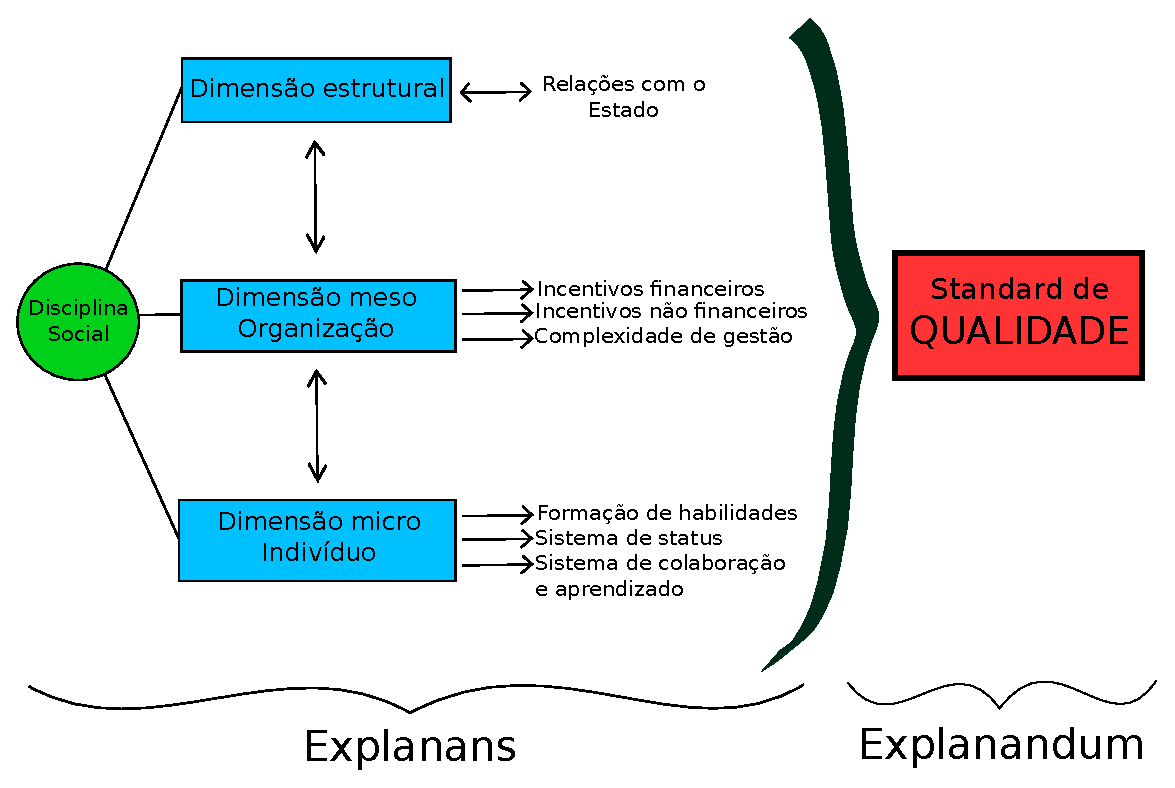
\includegraphics[scale=.8]{modelo_analise_tese.eps}
%		\fonte{Elaboração do autor.}
%	\end{figure}



	\section{ERGM}
	
	Os ERGM's, \cite{robins2007introduction,lusher2013exponential,lazega2014redes,brailly2017explorer}, são modelos estatísticos desenvolvidos especificamente para dados relacionais. Uma estrutura de relações postula interdependência entre as identidades que a compõem. Isso fere um dos pressupostos da modelagem estatística convencional, qual seja, a independência das informações. ``O fato de que eu escolho Pedro como amigo não é necessariamente independente do fato de que eu também escolho Paulo porque eles também podem ser amigos entre si \cite[p. 76]{lazega2014redes}.
	
	%ERGM's are statistical models developed specifically to deal with relational data \cite{robins2007introduction,lusher2013exponential}. A relations structure postulates interdependence between identities. This goes against one of the assumptions of conventional statistical modeling, the independence of information. ``The fact that I choose Peter as my friend is not necessarily independent of the fact that I also choose Paul because they can be friends with each other'' \cite[p. 76]{lazega2014redes}.
	
	Os ERGM's podem ser definidos por
	
	
	\begin{equation}
	Pr(Y=y) \quad = \quad \left(\frac{1}{k}\right) exp \left\{ \sum_{A} \eta_A g_A (\textbf{y}) \right\}
	\end{equation}
	
	onde $Y$ é o grafo teórico estimado, $y$ é o grafo observado, $\sum_{A}$ é a soma de todas as configurações \textit{A}, $\eta_A$ é o parâmetro estimado correspondente à configuração \textit{A}, $g_A(\textbf{y})$ é a estatística da rede correspondente à configuração \textit{A} no grafo \textbf{y} e \textit{k} é uma constante que assegura uma distribuição de probabilidade adequada\cite{robins2007introduction}. Esta família de modelos nos permite estimar o efeito de cada configuração endógena na emergência da própria rede. Dito de outra maneira, visto que cada configuração endógena pode ser associada a um processo social, este modelo nos permite \textit{explicar a rede como uma variável dependente}, explicar quais processos são importantes e quais são secundários para entender a estrutura social em investigação.
	
	%where Y is the theoretical estimated graph, y is the observed graph, $\sum_{A}$ is the sum of all configurations \textit{A},  $\eta_A$ is the estimated parameter corresponding to configuration \textit{A}, $g_A(\textbf{y})$ is the network statistic corresponding to configuration \textit{A} of graph \textbf{y} and \textit{k} is a constant that ensures an adequate probabilities distribution \cite{robins2007introduction}. This model allows us to estimate the effect of each endogenous configuration of the network on the emergence of the network itself. Put another way, since every endogenous configuration can be associated with a social process, the model allows us to \textit{explain the network as a dependent variable}, to explain which processes are important and which are not important to understand the social structure under investigation. In our case, this procedure will be conducted for both levels of the network, that is, we will model both social processes modeling the inter-individual structure and the inter-organizational structure.
	
	Para os fins deste trabalho, utilizaremos uma variação dos ERGM's conhecida como ``Modelos de Seleção Social'' (\textit{Social Selection Model}). Esses modelos foram propostos por \citeonline{robins2001network} com o objetivo de dar conta da heterogeneidade existente dentro das estruturas sociais usando atributos dos nós como covariáveis exógenas. Desse modo, além das configurações internas da própria rede, analisaremos ainda como variáveis exógenas moldam a emergência da estrutura \cite{wang2016social}.
	
	%In this research we will use a variation of the ERGM known as ``Social Selection Models''. These models were proposed by \citeonline{robins2001network} aiming to take account of the existing heterogeneity inside social structures using nodal attributes as exogenous covariables. Therefore, besides the network's own configurations, we will analyze how exogenous variables shape the emergence of the structure as well \cite{wang2016social}.
	
	
	\section{Transformações de redes de 2 modos}
	
	%2-mode to 1-mode transformations allow us to investigate an affiliation network anchored in the assumption that when people are engaged in the same organizations or in the same events (a common approach in the literature), people build ties between themselves. This procedure counts one tie between two organizations when they share a person or a tie between two persons when both are engaged in the same organization \cite{brailly2016market,lazega2014redes}. The result is a 1-mode weighted network of individuals who participate in the same organizations or a 1-mode weighted network of organizations that share members.
	
	Transformações de redes de 2 modos para 1 modo nos permitem investigar uma rede de afiliações ancorada no pressuposto de que quando as pessoas estão engajadas nas mesmas organizações ou nos mesmos eventos (uma abordagem muito comum na literatura), elas constroem laços entre si. De acordo com \citeonline{denooy2011exploratory}
	
	\begin{citacao}		
		Na ciência política, economia e sociologia, muita atenção tem sido dada à composição de conselhos em grandes corporações. (\dots) Se uma pessoa é membro de um conselho de diretores em duas companhias, ele ou ela (\dots) é um diretor múltiplo que cria um diretorado conectivo ou uma conexão entre firmas. A rede de diretorados conectivos nos diz algo sobre a organização de um setor de negócios. É assumido que diretorados conectivos são canais de comunicação entre firmas\footnote{In political science, economy, and sociology, much attention has been paid to the composition of the boards of large corporations. (\dots) If a person is a member of the board of directors in two companies, he or she (\dots) is a multiple director who creates an interlocking directorate or interlock between firms. The network of interlocking directorates tells us something about the organization of a business sector. It is assumed that interlocking directorates are channels of communication between firms.}. \cite[p. 117]{denooy2011exploratory}
	\end{citacao}
	
	
	O procedimento de transformação conta um laço entre duas organizações quando elas compartilham um indivíduo afiliado ou um laço entre duas pessoas quando ambas estão engajadas na mesma organização \cite{brailly2016market,lazega2014redes}. O resultado é uma rede ponderada de 1 modo de indivíduos que participam nas mesmas organizações ou uma rede ponderada de 1 modo de organizações que compartilham membros.
	

	
	
	\section{Dados relacionais}
	
	%Our study object presents itself as a multilevel structure: the meso/organizational level represented by social groupings, in this case, orchestras and organizations and their relations with the State, the micro, individual level and the affiliations between the two levels \cite{brailly2016market,eloire2009reseaux,lazega2008catching,favre2016inter,lazega2016synchronization}.
	
	Nosso objeto de estudo se apresenta como uma estrutura em rede multinível: o nível organizacional representado pelos grupos sociais, neste caso, as orquestras e demais organizações com quais elas mantém relação e o Estado, o nível individual composto aqui pelos músicos da cidade de Belo Horizonte e as afiliações entre os dois níveis.
	

	%The structure in the individual level, musicians, will be tracked from advisement networks\footnote{Cf. Appendix 2 - Sociometric online questionnaire - individuals.} (aiming to capture artistic prestige), friendship networks and job indication networks. We will adopt degree centrality, betweeness centrality and constraint as indicators for finding \textit{hubs}. We will also investigate some of the individuals' \textbf{attributes} such as country of origin, the city of origin, training institution and teacher along with demographic information. This indicators show us a little of the musicians' \textbf{context} and how he can be situated \textit{a priori} in a prestige scale within the field. The name generators will be as follows:
	
	A estrutura do nível individual será investigada a partir de redes de aconselhamento\footnote{Cf. Apêndice 2 - Questionário sociométrico online - indivíduos.} (com o objetivo de capturar o prestígio individual), redes de amizade, indicação para trabalhos e convites para se apresentar conjuntamente. Adotaremos a centralidade de grau, a centralidade de intermediação e o \textit{constraint} como indicadores para encontrar os \textit{hubs}. Investigaremos também alguns dos atributos individuais como país de origem, cidade de origem, instituição de treinamento musical e professor junto com algumas variáveis sociodemográficas. Esses indicadores nos mostram um pouco do contexto dos músicos e como eles podem ser situados \textit{a priori} numa escala de prestígio dentro do campo. Os geradores de nomes serão conforme o apresentado abaixo:
	
	\begin{enumerate}
		\item Se o(a) senhor(a) precisasse de aconselhamento sobre a interpretação de alguma peça, independente do período ou do estilo da obra, a quem o(a) senhor(a) pediria conselho? Mencione quantas pessoas o(a) senhor(a) quiser.
		\item O(a) senhor(a) costuma se encontrar com outros músicos em ocasiões sociais fora do horário de trabalho? Com quem o(a) senhor(a) se encontra? Mencione quantas pessoas o(a) senhor(a) quiser.
		\item Se o(a) senhor(a) fosse indicar um músico para uma excelente posição em uma orquestra, a quem o(a) senhor(a) indicaria? Mencione quantas pessoas o(a) senhor(a) quiser independente do instrumento.
		\item Se o(a) senhor(a) fosse responsável por organizar um recital ou um concerto no qual o(a) senhor(a) fosse tocar, independente da instrumentação das obras que o senhor poderia escolher, a quem o(a) senhor(a) convidaria para tocar com o(a) senhor(a)? Mencione quantas pessoas o(a) senhor(a) quiser.
	\end{enumerate}




	
	
	%\section{Proposta de indicadores}
	
	%Com o intuito de operacionalizar o desenho de pesquisa descrito supra, buscaremos os seguintes indicadores: para verificar o padrão de qualidade vigente, verificaremos a representação dos músicos dos atributos da qualidade. Para verificar o Ranking das orquestras, utilizaremos um conjunto de indicadores: a representação dos músicos sobre o Ranking, o preço médio do ingresso, a quantidade de concertos por temporada e o volume total de investimentos. O preço médio do ingresso é adotado aqui como uma \textit{proxy} da qualidade embasado no achado de \citeonline{throsby1983quality} (a demanda é inelástica em relação ao preço mas altamente correlacionada com relação á qualidade percebida). Argumentamos que esta é uma boa proxy pois as pessoas estariam dispostas a pagar mais por um concerto que percebem como sendo de alta qualidade. A quantidade de concertos e o volume total de investimentos parecem, à primeira vista, \textit{proxys} menos seguras do que a anterior pois percebe-se um risco de cair numa tautologia. As orquestras são boas porque tem mais financiamento ou tem mais financiamento porque são boas? Tocam mais porque são boas ou são consideradas boas porque tocam mais? Contudo, argumentamos que, se adotados com parcimônia e sempre conjugados a outras variáveis, esses indicadores podem dar \textit{insights} valiosos sobre o campo. Pretendemos testar um índice de qualidade criado a partir da aglutinação dessas variáveis através de uma análise fatorial\footnote{Em linhas muito gerais, a análise fatorial é uma técnica de análise multivariada que visa reduzir a complexidade dimnuindo as dimensões a serem analisadas em índices ou escores \cite{mingoti2005analise}.}.
	
	
	%Para capturar as interações no nível individual, construiremos redes relacionais entre músicos a partir de questionários sociométricos. Maiores detalhes sobre o questionário serão apresentados na seção seguinte. Por ora é suficiente indicar que adotaremos a centralidade de grau, centralidade de intermediação e o \textit{constraint} como indicadores para encontrar os \textit{hubs}. Os atributos dos indivíduos, as variáveis exógenas às redes, serão mensuradas pelo país de origem, cidade de origem, instituição de formação e o professor. Esses indicadores nos mostram um pouco do contexto do músico e de como ele pode ser situado a priori numa escala de prestígio em meio ao campo.
	
	%A estrutura de incentivos oferecida pela orquestra será mensurada através do salário médio e dos níveis salariais dos músicos\footnote{Pretendemos comparar entre orquestras tanto a média geral do salário quanto o salário por funções específicas, e.g., spalla e chefes de naipe que comumente ganham mais do que os demais músicos de seção.}. Os incentivos não financeiros serão mensurados pela quantidade de vezes em que um membro da orquestra se apresentou como solista ou teve um concerto de câmara agendado em nome da orquestra\footnote{É comum às orquestras organizarem concertos com formações menores como quartetos de cordas ou quintetos de metais com músicos selecionados entre seus membros.}. A complexidade da gestão será mensurada pela quantidade de setores e diretorias que a orquestra/instituição mantenedora possui e pela quantidade de níveis hierárquicos do instrumentista até o presidente.
	
	%Os indicadores escolhidos para mensurar o nível de interação com o Estado são o volume financeiro investido pelo próprio Estado e a existência/quantidade de contratos, convênios ou parcerias firmados.
	
	
	
	%The upper level is composed by the orchestras and all the other organizations with whom they maintain any kind of relation, whether it is an economic relation, a partnership or a resources exchange agreement\footnote{Cf. Appendix 3 - Sociometric questionnaire - organizations.}. We will track the organizations' main activity, it's style (in White's terms), it's formal structure and it's collaboration ties. The \textbf{incentive structure} offered by the orchestra will be measured through average salary and salaries of musicians\footnote{We intend to compare both the average salary and specific salary by function, e.g., concertmaster and other leaders inside the orchestra that commonly earn more money than the other section musicians.}. The \textbf{non-financial incentives} will be measured by the number of times an orchestra member played as a soloist or in a chamber music concert in the orchestras' season\footnote{It is common to professional orchestras to organize concerts with smaller ensembles as string quartets or brass quintets with selected musicians.}. The \textbf{management complexity} will be measured by the quantity of sections and boards that the orchestra/maintainer have and by the amount of hierarchical levels between the instrumentalist and the CEO.
	
	O nível organizacional é composto pelas orquestras e todas as outras organizações com as quais elas mantêm algum tipo de relação, seja uma relação econômica, uma parceria ou uma troca de recursos\footnote{Cf. Apêndice 3 - Questionário Sociométrico - organizações.}. Investigaremos a principal atividade das organizações, seu estilo (nos termos de White), sua estrutura formal e seus laços. Os incentivos não financeiros serão investigados pela quantidade relativa de vezes que os membros da orquestra se apresentaram como solistas ou em concertos de câmara durante a temporada\footnote{É comum as orquestras profissionais organizarem concertos com grupos menores como quartetos de cordas ou quintetos de metais com músicos selecionados.}. A complexidade organizacional será mensurada pela quantidade de setores ou diretorias que a orquestra possui e pelo número de níveis hierárquicos que separam os músicos do CEO.
	
	
	%Table \ref{indicadores-relational} show a synthesized version of the proposed indicators regarding the relational data and the organizational level.
	
	A Tabela \ref{indicadores-relational} mostra uma versão sintetizada dos indicadores propostos relacionados aos dados relacionais nos níveis individual e organizacional.
	
	%Os indicadores aqui elencados estão apresentados de forma resumida na Tabela \ref{indicadores}. Seguimos apresentando os dados a serem coletados e os métodos de análise utilizados.
	
	
	\begin{table}
		\ibgetab{
			\centering
			\caption{Indicadores propostos - dados relacionais}
			\label{indicadores-relational}
		}
		{\begin{tabular}{|c|c|}
				
				\hline
				\textbf{Conceito - Nível individual} & \textbf{Indicador} \\
				\hline
				Interação individual & Redes \\
				\hline
				Atributos individuais de interesse & País de origem  \\
				& Cidade de origem  \\
				& Insituição de formação \\
				& Professor    \\
				\hline
				Informações demográficas & Idade \\
				& Sexo \\
				& Renda total \\
				& Escolaridade \\
				& Cor da pele \\
				& Estado civil \\
				& Número de filhos \\
				& Principal atividade profissional \\
				\hline
				\textbf{Conceito - Nível organizacional} & \textbf{Indicador} \\
				\hline
				Interação organizacional & Redes \\
				\hline
				Incentivos não financeiros & Convites para solista \\
				& Convites para concertos de câmara \\
				\hline
				Complexidade Organizacional  & Número de setores/diretorias  \\
				& Distância em níveis entre os músicos e o CEO \\
				\hline
				
			\end{tabular}
		}
		{\fonte{Elaborado pelo autor.}}
	\end{table}
	
	



	\section{Síntese teórica}

	% White - qualidade
	Neste trabalho, procuramos entender o funcionamento dos mercados de produção da música de concerto, bem como suas bases operacionais. Aqui, os mercados serão analisados como estruturas em rede \cite{white2002markets}. A disciplina em torno da qual funciona o mercado da música orquestral é uma \textit{interface} e sua ordem de valor é dada pela \textbf{qualidade} \cite{white2002markets}. A qualidade é reguladora da ação conjunta pois todos os participantes do mercado seja qual for sua natureza (indivíduos ou organizações) tiram dela suas bases normativas básicas da vida social imbuídas na estrutura. Dito de outra forma, é a partir da qualidade percebida e do \textit{Ranking} de orquestras advindo da escala de qualidade como marco regulatório (a interface do mercado) que os agentes (identidades) agem sobre a estrutura em que estão. A qualidade, entretanto, não é algo inerente às organizações mas um atributo que emerge de múltiplas interações tanto no nível das organizações quanto no nível dos indivíduos. Explicar como emerge a qualidade no mercado das orquestras configura o centro desta investigação.

	% Estado
	Para além da disciplina, o mercado da música orquestral encontra no Estado o seu segundo articulador mais importante.	De acordo com \citeonline{fligstein2002architecture}, o Estado possui um papel fundamental na regulação e, consequentemente, na estabilização dos mercados. No contexto brasileiro, a máquina estatal figura como principal financiador das orquestras mesmo que atuando de forma indireta (através das leis de incentivo à cultura). As leis de incentivo à cultura funcionam como catalisadores da produção cultural no país (quer seja a nível federal, estadual ou municipal) e fora do seu escopo há poucas produções acontecendo e mais voltadas ao entretenimento. As únicas produções que são capazes de subsistir prescindindo desse mecanismo de financiamento são, normalmente, grandes shows ou grandes espetáculos promovidos por grandes empresas.

	% Nível da organização - incentivos financeiros e não financeiros, capacidade de gestão
	Mais ao nível da organização, é possível apontar algumas atributos que exercem influência sobre a construção de sua identidade e, consequentemente, seu posicionamento na estrutura mercantil. São eles os \textit{incentivos financeiros}, os \textit{incentivos não financeiros} e a capacidade de gestão da organização ou de sua instituição mantenedora. Suspeitamos que haja uma forte correlação entre o salário pago pelas orquestra e a percepção de seu posicionamento no \textit{Ranking} de qualidade. Do mesmo modo, as orquestras podem criar sistemas de incentivos aos músicos onde o retorno pode passar tanto pelo prestígio quanto pela realização pessoal. Uma audição interna para a escolha de um solista para um dos concertos na temporada ou uma foto de um músico estampada no encarte mensal são exemplos de incentivos não financeiros. Finalmente, quando nos referimos à capacidade de gestão da instituição, estamos visando sua estrutura formal. É razoável pensar que uma organização que possua uma estrutura formal mais complexa será melhor avaliada no \textit{Ranking} da qualidade do que organizações com estruturas formais mais simples. O discurso comum no campo é de que ``orquestras mais organizadas são melhores''.

	% isomorfismos
	Segundo \citeonline{dimaggio1983iron}, as organizações se engajam em processos que as levam a se tornarem cada vez mais parecidas. Esses isomorfismos acontecem como estratégia de estabilização e segurança contra as incertezas do mercado. No caso das orquestras, isso parece ser uma estratégia de diferenciação em nichos de mercado claramente perceptíveis, sobretudo no que toca ao estilo de especialidade da orquestra. Hoje, há orquestras especializadas em música antiga, em música contemporânea, em música \textit{pop}, etc.


	% coopetição
	Vimos que no exercício cotidiano de suas atividades, embora estejam em situação de competição, as organizações entram em processos supraintencionais de cooperação como estratégia que visa a estabilização do mercado, o que ficou conhecido como \textit{coopetição} \cite{lazega2009theorie}. No mercado das orquestras esse processo pode acontecer tanto por trocas de recursos (partituras, equipamentos, ajudas financeiras propriamente dito) quanto por trocas de informação e conhecimento. Músicos que tocam em mais de uma orquestra, regentes e solistas convidados podem ser alavancas para trocas de informação e conhecimento.

	Mais ao nível do indivíduo, podemos indentificar alguns atributos que possam ter influência na qualidade atribuída a uma determinada orquestra. Esses atributos passam pelas habilidades adquiridas pelos músicos onde entram tanto o seu ambiente de formação quanto o seu professor (a construção das habilidades artísticas do músico, argumentamos, possuem tanto uma dimensão técnica relacionada à sua habilidade de tocar propriamente dita, quanto uma dimensão simbólica associada ao prestígio de seu professor e da instituição de ensino que frequentou). Além disso, no nível da interação é que podemos verificar um sistema de status entre músicos e um sistema de colaboração e aprendizado.

	Dadas essas breves definições iniciais, podemos explicitar algumas proposições centrais que nortearão a condução de nosso pensamento: (1) Os mercados de produção da música orquestral operam e encontram sua estabilização ancorados num padrão de qualidade comum com o qual todos assumem compromisso. Esse padrão de qualidade também dá origem a um ordenamento interorganizacional que reflete a interface do mercado e que é amplamente reconhecido. (2) A qualidade, o principal mecanismo articulador da estrutura, emerge do próprio mercado no fluxo das interações entre organizações e agentes. Os agentes com maior peso na emergência da qualidade são os professores e os \textit{hubs}, músicos com grande centralidade na estrutura.

	Apresentaremos agora nossas principais hipóteses de trabalho.
	
	\section{Hipóteses}
	
	\newtheorem{hip}{Hipótese}

	%We depart from the central assumption that the quality standard, the gravity center of orchestras' market, emerges from its own structure. At the individual level, we argue that the concepts of a ``good orchestra'', a ``good performance'', a ``good instrumental technique'', emerge from the bottom up and not from top down. Also, that seems to be a struggle for the ``right'' to the definition of quality. This leads us to hypotheses regarding individuals, organizations and their relation with the State.
	
	Partimos do pressuposto central de que o padrão de qualidade, o centro gravitacional do mercado das orquestras, emerge de sua própria estrutura. No nível individual, argumentamos que os conceitos de ``boa orquestra'', ``boa performance'', ``boa técnica instrumental'', emergem de baixo para cima e não de cima para baixo. Além disso, parece haver uma disputa pela ``correta'' definição da qualidade. Isto nos leva a hipótese relacionadas aos indivíduos, às organizações e a suas relações com o Estado.
	
	\begin{hip}
		Quanto maior a importância de um músico dentro de sua rede interpessoal (em termos de popularidade, atividade e liberdade de ação), maior será sua influência na construção do padrão de qualidade.
	\end{hip}
	

	
	\begin{hip}
		%The more an orchestra provides structural incentives for the musicians, the better it will be positioned in quality ranking.
		Quanto mais uma orquestra provê incentivos estruturais para os músicos, melhor ela estará quanto ao seu posicionamento no ranking de qualidade percebido.
	\end{hip}
	
	%Quanto mais incentivos as orquestras proporcionam a seus músicos, mais elas tendem a ocupar as primeiras posições no Ranking de qualidade.
	
	\begin{hip}
		%The more complex the organizational structure of an orchestra or of its maintainer, the better it will be positioned in quality ranking.
		Quanto mais complexa for a estrutura organizacional de uma orquestra ou de sua mantenedora, melhor ela estará quanto ao seu posicionamento no ranking de qualidade percebido.
	\end{hip}
	
	\begin{hip}
		%The more complex an orchestra's business network, the better it will be positioned in quality ranking.
		Quanto mais complexa a rede de negócios de uma orquestra, melhor ela estará quanto ao seu posicionamento no ranking de qualidade percebido.
	\end{hip}
	
	
	%Por fim, num nível macro, o nível do próprio mercado e sua relação com o Estado, argumentamos que
	Por fim,
	
	\begin{hip}
		%The closest the relationship of an orchestra with the State, the better it will be positioned in quality ranking.
		Quanto mais próximas as relações de uma orquestra com o Estado, melhor ela estará quanto ao seu posicionamento no ranking de qualidade percebido.
	\end{hip}







\begin{comment}
	\section{Dados e Métodos}



	Para realizar nossa investigação identificaremos as orquestras da cidade de Belo Horizonte incluindo sua região metropolitana e sua rede de parceiros comerciais. A escolha de Belo Horizonte se deu tendo em vista seu número relativamente pequeno de orquestras profissionais (em torno de seis), o que viabiliza o trabalho de campo, além de sua reconhecida expressividade no cenário cultural nacional.



	À luz da perspectiva relacional, buscaremos entender o fluxo de recursos e informação nessa estrutura permitindo a produção da música orquestral. Essa parte da pesquisa será realizada por meio de investigações preliminares do conteúdo a respeito das orquestras disponível \textit{online}, entrevistas com os gestores da organização e visitas \textit{in loco}.



	Para investigar a construção social do padrão de qualidade vigente na estrutura do mercado, adotaremos duas estratégias de pesquisa. A primeira está ancorada no pressuposto de que parte dos mecanismos cognitivos e de controle da qualidade acontecem na socialização realizada nos anos de formação acadêmica dos músicos. Dito de outra forma, os músicos aprendem com seus professores de graduação o que é uma performance boa e uma ruim, o que é uma orquestra boa e uma ruim, quais são os critérios que entram na avaliação da qualidade artística de um músico, etc. Muito embora essa concepção possa (e provavelmente vai) mudar ao longo da carreira de um músico em seus movimentos de acoplar e desacoplar dos diversos domínios em rede que participará, a base conceitual construída junto ao professor tende a criar raízes fortes. Desse modo, a primeira estratégia consiste em realizar entrevistas semiestruturadas com os professores de graduação em música das universidades em Belo Horizonte. Não será feito nenhum procedimento estatístico de amostragem devido ao caráter mais qualitativo dessa etapa da pesquisa. Adotaremos, portanto, uma amostragem por julgamento tendo em conta o conhecimento prévio do autor sobre os professores da cidade. O objetivo das entrevistas é verificar convergências no discurso dos professores acerca do que é uma boa performance e uma orquestra de qualidade. A segunda estratégia está ancorada no pressuposto de que o padrão de qualidade emerge de um sistema de status presente na estrutura hierarquizada dos músicos. Numa rede qualquer, os diversos indivíduos se estratificam numa hierarquia de prestígio e status e os indivíduos mais prestigiosos costumam mobilizar os critérios de qualidade. Desse modo, investigaremos a estrutura relacional entre os músicos das diversas orquestras identificando os nós mais centrais. Considerando o número alto de músicos profissionais em Belo Horizonte, julgamos que a abordagem mais apropriada e com maiores chances de retorno consiste da elaboração de um questionário sociométrico \textit{online}. Na ocasião de uma das visitas feitas às orquestras, este autor terá um momento com os músicos para explicar de maneira detalhada o teor do trabalho bem como a importância de sua colaboração ao que se seguirá o envio dos questionários. Após a identificação dos indivíduos com alta centralidade na rede, buscaremos entrevistá-los de maneira semelhante aos professores.



	%%% Repensar o trecho abaixo. Não sei se vai dar para aplicar a pesquisa em Hastings e em Paris. Pouco tempo e, no caso de Paris, a vida cultural é imensa.



	%A mesma pesquisa será realizada em duas cidades fora do Brasil, a saber, Paris (França) e Hastings (Inglaterra). A visita a essas cidades acontecerá subsidiada pela CAPES via Bolsa de Doutorado Sanduíche no Exterior\footnote{Agradeço à CAPES pela concessão da referida bolsa, o que torna possível o estudo comparado do mercado das orquestras no Brasil e nas duas cidades Europeias.}. A primeira cidade será residência doutoral deste autor de outubro de 2017 a janeiro de 2018. Nessa ocasião, empreenderemos o mesmo procedimento de pesquisa a ser realizado no Brasil, i.e., entrevistas com os gestores e músicos das orquestras e visitas \textit{in loco}. Essa cidade é pertinente para uma comparação com o contexto Brasileiro tendo em vista sua efervescência cultural, sua proeminência no cenário europeu e sua aparente semelhança ao modelo brasileiro de financiamento.



	%A cidade de Hastings, por outro lado, representa um caso paradigmático divergente das outras duas investigadas. Ela possui apenas uma orquestra profissional, a Hastings Philharmonic\footnote{\url{http://www.hastingsphilharmonic.com}}, com aproximadamente dois anos de funcionamento. Em conversas informais com o maestro dessa organização, ele nos relatou que o surgimento da orquestra mobilizou um mercado quase inexistente na cidade. ``As pessoas que desejavam assistir a um concerto deveriam viajar por duas horas de trem para Londres'', comenta. O principal slogan promocional da orquestra é ``a mais nova orquestra profissional de \textit{South East} desde a 2ª Guerra''. Acreditamos que a investigação dessa organização nos dará excelentes dados para compreender a emergência de um mercado.





	%%%% Descrever o roteiro de entrevistas dos professores e o questionário sociométrico aplicado aos músicos.



	A proposta de roteiro de entrevistas está apresentada no Anexo 2. O questinário online enviado aos músicos está apresentado em detalhes no Anexo 3. Após levantamento de atributos do entrevistado, identificaremos redes de aconselhamento (visando capturar o prestígio artístico),redes de amizade e redes de indicação profissional. Excluiremos aqui redes de coparticipação em performances por acreditarmos que elas resultarão em um dado demasiado redundante, visto que os questionários serão enviados para músicos de orquestras, e custoso para os entrevistados, dado o enorme número de músicos com os quais uma pessoa pode se apresentar.









	\section{Modelos analíticos relacionais}



	As análises se darão através de dois tipos de modelagem em redes: os modelos de blocos, ou \textit{blockmodeling} e os ERGM, ou modelos P* (modelos estatísticos específicos para dados relacionais). Explicitaremos sucintamente a racionalidade por trás desses modelos e como eles serão úteis na análise dos dados supracitados.



	\subsection{Blockmodeling}



	Os \textit{blockmodels} são uma operacionalização de um dos conceitos centrais na análise de redes, qual seja, a equivalência estrutural. Este conceito baseia-se na ideia de que indivíduos podem exercer papeis sociais numa estrutura em rede a partir de posições específicas \cite{lazega2014redes}. Os modelos de blocos utilizam, na maioria das vezes, correlações iteradas sobre as linhas e colunas de uma matriz relacional ou a medida da distância euclidiana para separar nós estruturalmente equivalentes. Para \citeonline{lazega2009theorie}, os \textit{blockmodels} são a melhor ferramenta disponível hoje para a investigação de nichos de mercado.



	Neste trabalho utilizaremos uma versão estocástica frequentista do modelo elaborada por \citeonline{daudin2008mixture} e uma versão estocástica bayesiana elaborada por \citeonline{latouche2012variational}.



	\subsection{ERGM}



	Os ERGM's, ou modelos P* \cite{robins2007introduction,lusher2013exponential,lazega2014redes,brailly2017explorer}, são modelos estatísticos desenvolvidos especificamente para dados relacionais. Uma estrutura de relações postula interdependência entre as identidades que a compõem. Isso fere um dos pressupostos da modelagem estatística convencional, qual seja, a independência das informações. ``O fato de que eu escolho Pedro como amigo não é necessariamente independente do fato de que eu também escolho Paulo porque eles também podem ser amigos entre si \cite[p. 76]{lazega2014redes}.



	O modelo P* pode ser definido por



	%\begin{equation}

	$$Pr(Y=y) \quad = \quad \left(\frac{1}{k}\right) exp \left\{ \sum_{A} \eta_A g_A (\textbf{y}) \right\}$$

	%\end{equation}



	onde Y é o grafo teórico estimado, y é o grafo observado, $\sum_{A}$ é a soma de todas as configurações \textit{A},  $\eta_A$ é o parâmetro estimado correspondente à configuração \textit{A}, $g_A(\textbf{y})$ é a estatística da rede correspondente à configuração \textit{A} do grafo \textbf{y} e \textit{k} é uma constante que assegura a distribuição de probabilidades adequada \cite{robins2007introduction}.



	Para os fins deste trabalho, utilizaremos uma variação do modelo P* conhecida como ``modelo de seleção social'' (\textit{Social Selection Model}). Esses modelos foram propostos por \citeonline{robins2001network} com o objetivo de dar conta da heterogeneidade existente dentro das estruturas sociais usando atributos dos nós como covariáveis exógenas. Desse modo, além das configurações internas da própria rede, analisaremos ainda como variáveis exógenas moldam a emergência da estrutura \cite{wang2016social}.


	%O trabalho está dividido da seguinte forma: no primeiro capítulo, faremos uma breve contextualização da formação do campo de investigação da sociologia econômica apresentando seus principais problemas e métodos e concluindo com a apresentação da literatura que proporciona a base teórica da investigação. No segundo capítulo, apresentaremos uma descrição profunda e detalhada da articulação do mercado de música erudita na região sudeste do Brasil. Apresentaremos cada ator, seu papel na rede, seus principais laços e suas linhas de atuação.



	%No terceiro capítulo, analisaremos com maior profundidade a rede de produção da música de concerto bem como o material etnográfico coletado durante o processo de pesquisa. No quarto capítulo, nos deteremos sobre os processos que envolvem a construção social da qualidade percebida nas orquestras ao que se segue nossas considerações finais.



	%Passemos à análise específica da economia que envolve grupos orquestrais.



	%\subsection{As orquestras}



	%\apudonline{volpe1991gap}{luksetich2011orchestras} desenvolveu em sua tese de mestrado um modelo para testar se a composição da carta de produtos oferecidos por uma orquestra influencia sua renda. Esse autor encontrou que, em sua amostra composta por diversas orquestras americanas segundo a classificação de orçamento da \textit{American Symphony Orchestra League} (ASOL), o buraco entre custos e receitas diminuía. Nas orquestras pequenas, esse buraco era ainda mais sensível à carta de concertos oferecidos. O autor conclui que há controle (pelo menos em algum nível) das orquestras sobre seu estado deficitário. \apudonline{brooks2000income}{luksetich2011orchestras} encontrou que a superação desse buraco era diferente para orquestras de porte diferente: as orquestras maiores, para controlarem seus déficits, deveriam diversificar os produtos oferecidos e investir em tecnologia e programas educacionais enquanto orquestras menores deveriam expandir sua atuação filantrópica. O envolvimento com ações educacionais e formativas parece ser atualmente senso comum entre as orquestras profissionais. Diversos projetos como os ``concertos didáticos'', máster-classes, e visitas de alunos do ensino fundamental e médio às instalações das orquestras acontecem com boa frequência nas programações. É curioso notar ainda que algumas das principais orquestras no mundo, como veremos, tem adotado com afinco a estratégia de desenvolvimento tecnológico, como a orquestra ``Philharmonia'' de Londres. Essa instituição, além de manter uma atuação constante em diversas mídias sociais populares (Facebook, Instagram, Twitter, etc.) e alimentar canais de transmissão de vídeos via \textit{streaming} (YouTube, Vimeo, etc.), desenvolveram um aplicativo para dispositivos móveis pioneiro intitulado \textit{The Orchestra App}\footnote{www.philharmonia.co.uk/app} onde os usuários podem assistir a um repertório 8 obras emblemáticas da música orquestral optando por visualizar o maestro, algum instrumento específico, acompanhar com a partitura simultaneamente dentre diversas outras possibilidades. O próprio maestro titular, Esa-Pekka Salonen, que também é um compositor de renome, desenvolveu um aplicativo para dispositivos móveis com funções de edição de partituras e gravação.



	%Partindo da constatação de que as artes de performance tem um custo fixo bastante alto em relação a seus custos marginais e que não há preço de ingresso que possa cobri-los \apud{hansmann1981nonprofit}{luksetich2011orchestras}, alguns estudos em economia da cultura tem se preocupado em entender a formação do preço e a demanda nesse contexto \cite{lange1984demand,luksetich1995simultaneous,felton1992assumed,felton1994evidence,seaman1987price}. Outros estudos tem investigado os procedimentos de contratação de músicos e sua relação com a diminuição da desigualdade de gênero nas instituições orquestrais \cite{goldin1997orchestrating}, o efeito da educação e do capital social sobre a empregabilidade e remuneração dos maestros \apud{ciocoiu2009schooling}{luksetich2011orchestras},  as diferenças entre orquestras estatais e privadas \cite{boyle2007ownership} e fatores determinantes de escolha de repertório \cite{luksetich2008effects}. A discussão sobre orquestras estatais e privadas no Brasil é recente visto que algumas das principais orquestras do país adotam um modelo de gestão onde uma instituição de terceiro setor é mantenedora e os músicos são contratados por CLT\footnote{Consolidação das Leis do Trabalho.} abandonando o modelo vigente até meados a década de 1990 quando os grupos orquestrais eram, em sua grande maioria, compostos de funcionários estatais. É senso comum, entre gestores e maestros, que essa mudança teve um impacto profundo na produtividade e na qualidade dos trabalhos. Até o momento, excetuando-se \citeonline{arruda2010parcerias} e \citeonline{carvalho2012organizaccoes}, desconheço outras investigações sobre o assunto.



	%Parte dos estudos em economia da cultura destina-se a investigar os objetivos das instituições orquestrais. Segundo \citeonline{luksetich2011orchestras}



	%\begin{citacao}

	%	A teoria econômica assume que indivíduos são maximizadores e empresas privadas com fins lucrativos são maximizadoras do lucro. Visto que as instituições sem fins lucrativos não podem distribuir qualquer excedente entre os donos ou organizadores da instituição, é geralmente assumido que elas tendem a maximizar sua produção, qualidade, orçamento, ou alguma combinação desses objetivos\footnote{Economic theory assumes that individuals are maximizers and private for-profit business firms are profit-maximizers. Since non-profits cannot distribute any surplus over costs to the owners or organizers of the instituion, it is generally assumed that they are likely to maximize their output, quality, budget, or some combination of these goals.}. \cite[p. 323]{luksetich2011orchestras}

	%\end{citacao}



	%\apudonline[p. 323]{lange1986managerial}{luksetich2011orchestras} mostraram que ``orquestras grandes investiram fundos sem restrições de uma maneira consistente com objetivos maximizadores de qualidade\footnote{(\dots) major orchestras spent unrestricted funds in a manner consistent with quality-maximization goals.}''.



	%\begin{citacao}

	%	Pareceu que a maximização do orçamento e a maximização da qualidade eram objetivos complementares no caso das orquestras maiores. Estimativas mostraram que tanto orquestras metropolitanas quanto orquestras de mercado menor tiveram maximização da produção como seu objetivo principal. Em ambos os casos, as concessões incondicionais recebidas pelas orquestras eram positivamente relacionadas ao número de concertos, o qual por sua vez resultou em maior público\footnote{It appeared that budget-maximizing and quality-maximizing were complementary goals in the case of the major orchestras. Estimates showed that both the metropolitan and the smaller market orchestras had output maximization as their major goal. In both cases, the unconditional grants received by orchestras were positively related to the number of concerts, which in turn resulted in greater attendance.}. \cite[p. 323]{luksetich2011orchestras}

	%\end{citacao}



	%\citeonline{brooks1999public} investigando concessões estatais às orquestras sinfônicas encontrou que elas são independentes das doações privadas. (EXPLICAR\ldots)



	%Vejamos \ldots



	%Em um estudo de 2006, \citeauthoronline{peacock2006arts} analiza de que modo é possível pensar em políticas públicas culturais considerando o cenário dinâmico e as recentes mudanças do setor e a ``soberania do consumidor''. Para esse autor, as principais mudanças do campo nos últimos anos podem ser resumidas da seguinte maneira: a abertura do conceito de comportamento econômico imbricado numa análise de bem-estar social (\textit{welfare state}); o problema de como respeitar o pressuposto da ``soberania do consumidor'' como critério inicial de valor, o que faz com que o mercado da arte falhe na distribuição dos bens culturais não conseguindo atingir um equilíbrio ótimo de Pareto. \citeonline{peacock2006arts} aponta como solução ao problema o completo abandono do pressuposto baseando-se no conceito de necessidade meritória (\textit{merit wants}) como cunhado por \apudonline{musgrave1987merit}{peacock2006arts}. A ideia de necessidade meritória assume que os membros da sociedade desenvolvem preferências em comum o que leva a um entendimento coletivo sobre o modo de satisfazê-las mesmo contrariando opiniões individuais a respeito. (p. 1093 do PDF)



	%Segue \ldots



	\begin{comment}





	\subsection{A perspectiva da sociologia econômica}

	\ldots













	\citeonline{white1993canvases} conduziram um estudo sobre a mudança técnica e sobre as carreiras dos pintores franceses do séc. XIX dando origem à chamada escola ``impressionista''. Para esses autores,



	\begin{citacao}

		A arte não é um tipo de brinquedo manipulado em seu desenvolvimento por forças sociais e econômicas. Mesmo assim, pintores mostram grande interesse em como se tornarem reconhecidos e viver de sua arte. Os padrões e relações no trabalho desses indivíduos tornam-se possíveis e são controladas por pressões institucionais das quais nenhum homem está apercebido. Os quadros e carreiras dos indivíduos mudam e são mudados pelas instituições peculiares ao mundo da arte\footnote{Art is not a kind of tinkertoy manipulated in its development by social and economic forces. Yet, individual painters do show deep interest in how to become recognized and make a living. The patterns and relations in the work of these individuals are made possible and are constrained by institutional pressures of which no one man is quite aware. The canvases and careers of individuals change and are changed by the institutions peculiar to the art world.}. \cite[p. xxi]{white1993canvases}

	\end{citacao}



	Esses autores entendem o sistema institucional como uma ``rede persistente de crenças, costumes e procedimentos formais que juntos formam uma organização social mais ou menos articulada com um objetivo central conhecido – aqui a criação e reconhecimento da arte\footnote{(…)a persistent network of beliefs, customs, and formal procedures which together form a more-or-less articulated social organization whit an acknowledged central purpose – here the creation and recognition of art.}'' \cite[p. 2]{white1993canvases}.



	Pierre Bourdieu tem também uma contribuição significativa nessa área de estudos. O autor desenvolveu o conceito de ``campo'' para estudar diversas ramificações do mundo econômico: o mercado imobiliário \cite{bourdieu2005social}, o campo científico \cite{bourdieu2008ciencia}, e o campo literário \cite{bourdieu2005regras} para citar alguns exemplos. Para Bourdieu



	\begin{citacao}

		Quando falamos de um \textit{campo} de tomadas-de-posição, estamos insistindo que o que pode ser constituído como um \textit{sistema} pelo bem da análise não é o produto de uma intenção de buscar coerência ou um consenso objetivo (mesmo se isso pressupõe concordância inconsciente ou princípios comuns) mas o produto e prêmio de um conflito permanente; ou, para colocar de outra forma, que o princípio gerativo, unificador desse 'sistema' é a luta, com todas as contradições que ele engendra\footnote{When we speak of a \textit{field} of position-takings, we are insisting that what can be constituted as a \textit{system} for the sake of analysis is not the product of a coherence-seeking intention or an objective consensus (even if it presupposes unconscious agreement of common principles) but the product and prize of a permanent conflict; or, to put it another way, that the generative, unifying principle of this 'system' is the struggle, whit all the contradictions it engenders.}. \cite[p. 34]{bourdieu1993field}

	\end{citacao}



	Num estudo sobre compositores de trilha sonora na indústria cinematográfica de Hollywood, \citeonline{faulkner2003music} busca entender de que forma compositores se associam a produtores de cinema dando origem às redes de produção hollywoodianas, quais são os compositores mais centrais no sistema e quais deles, por conseguinte, tem domínio sobre a rede. Para isso, além de uma grande pesquisa etnográfica, o autor monta uma matriz de afiliação indicando quais compositores trabalharam com quais produtores e, com uso de um \textit{blockmodeling}, separa ambos os profissionais em quatro subgrupos onde os membros de um mesmo grupo são estruturalmente equivalentes. Para dividir os compositores em um mesmo subgrupo o critério usado pelo autor foi de consistência, não conectividade. Por exemplo:



	\begin{citacao}

		Fred Karlin e Michael Small são figuras grandes e centrais em Hollywood. Eles compuseram para filmes de um mesmo produtor ao longo dos doze anos. Os pontos de trabalho em suas linhas de carreira convergem. Na medida em que eles ``compartilham'' subgrupos de cineastas, são mais propensos a aparecer juntos na matriz da Grande Hollywood. Os compositores Karlin e Small trabalharam para o produtor e diretor Alan J. Pakula, cujos créditos incluem \textit{The sterile Cuckoo} (1969), \textit{Klute} (1971), \textit{The Parallax View} (1974), \textit{All the President's Men }(1976), e antes, \textit{Up the Down Staircase }(1967), \textit{The Stalking Moon }(1968), e \textit{Love with the Proper Stranger }(1963). Se o compositor David Shire se junta a Karlin e Small, como fez quando compôs a trilha para o sucesso \textit{All the President's Men}, ele é mais propenso a mostrar um padrão de equivalência em suas conexões a essa parte do mercado, a parte ou nicho feita pelos filmes de Alan Pakula e suas seleções de compositores para esses filmes.



		Similarmente, quando John Williams é contratado pelo cineasta Walter Mirisch, e Jerry Fielding e John Mandel são também contratados por Mirisch, há um padrão de conexões comuns entre os três a este, um cineasta altamente produtivo. Todos os três estão consistentemente ligados a um empregador comum. Todos os três foram sujeitos ao controle de Mirisch como empregador e como um ``cliente'' para seus serviços.



		De acordo com que ``sets'' múltiplos de produtores de filme, como Pakula e Mirisch, contratam os serviços de freelancers como Shire, Karlin, Williams, Fielding, Mandel e Small, um padrão de equivalência começa a emergir. \cite[p. 186]{faulkner2003music}

	\end{citacao}



	Com essa análise, Faulkner consegue identificar quais são os compositores que tem o mesmo padrão de conexões com produtores. Adicionando a essa informação medidas de produtividade (quais deles tem o maior número de créditos) e de reconhecimento (quais deles tem indicações e vitórias no Oscar, quais filmes cujas trilhas foram compostas por eles foram indicados e ganharam o Oscar), o autor identifica quais são os principais compositores do mercado de filmes em Hollywood, aqueles que tem o controle do sistema.



	Seguiremos a linha de análise desenvolvida por \citeonline{white1993canvases} e \citeonline{becker2008art} no que tange os processos de produção e distribuição pelo fato de esses autores, como já dito, entenderem o sistema de produção da arte como redes de cooperação.



	\end{comment}



	\begin{comment}





	\subsection{O Mercado dos Concertos}



	Compreender o mercado da música de concerto exige entendimento acerca das convenções vigentes, dos recursos que são mobilizados no processo de cooperação entre atores e como esses recursos circulam na rede, da distribuição/comunicação das instituições artísticas envolvidas, do papel dos críticos na formação de opiniões, do papel do Estado como regulador e principal financiador, dos processos de mudança no mundo da música de concerto e da construção da reputação dos atores envolvidos. Discorreremos brevemente acerca desses pontos. Características relevantes do público frequentador e sua influência no consumo dos concertos serão abordadas oportunamente.



	Para \citeonline{becker2008art} as convenções exercem grande controle sobre os artistas em virtude de sua complexidade sistêmica; para que alguma convenção sofra mudança, uma diversidade de outras mudanças é necessária. ``Um sistema de convenções toma corpo em equipamentos, materiais, treinamento, espaços e lugares disponíveis, sistemas de notação, e similares, os quais devem ser mudados se qualquer componente é mudado \footnote{A system of conventions gets embodied in equipment, materials, training, available facilities and sites, systems of notation, and the like, all of which must be changed if any one component is.}'' \cite[p.32]{becker2008art}. Se um compositor escreve uma música num sistema de 42 microtons dentro de uma oitava ao invés do sistema habitual de doze semitons, surge a necessidade da construção de instrumentos específicos para que essa música seja tocada. Os instrumentos ocidentais em sua grande maioria não são capazes de produzir intervalos menores do que um semitom (algumas exceções seriam os instrumentos da família das cordas pelo fato de não serem temperados\footnote{Em outra oportunidade, estudamos de que modo o processo chamado de temperamento dos intervalos da série harmônica e a consequente forma de construção dos instrumentos ocidentais modernos dão corpo ao processo de racionalização da música ocidental \cite{weber1995fundamentos}}). Algumas obras de Villa-Lobos, para citar outro exemplo, fazem uso de instrumentos de percussão nunca antes utilizados e inspirados em instrumentos dos índios da Amazônia. Quando da apresentação dessas obras, os percussionistas da orquestra precisam construir os instrumentos a partir de orientações deixadas por Villa-Lobos.



	Além dos recursos financeiros necessários, uma longa lista pode ser feita abarcando recursos materiais e recursos humanos (\textit{personnel}). \citeonline{becker2008art} comenta a respeito do controle que os artistas podem sofrer em seu processo criativo no caso de um alto nível de especialização técnica ou monopolização de recursos dos colaboradores:



	\begin{citacao}

		Eles [os artistas] escolhem do conjunto do que está disponível para eles no mundo da arte em que trabalham. Os mundos diferem em o que eles tornam disponível e na forma pela qual tornam-no disponível. Os padrões de atividade econômica característicos de uma sociedade moldam com o que os artistas podem trabalhar e com quem eles podem trabalhar. Fatos como o grau de monopolização da produção de materiais, a rentabilidade de mercados menores e o grau no qual os artistas precisam de itens especialmente desenhados e manufaturados para eles afeta o que está disponível e, portanto, o que os artistas podem fazer. Similarmente, as organizações pelas quais o pessoal de suporte encontra os projetos nos quais trabalham criam motivos organizacionais, profissionais e de carreira que podem ir de encontro às intenções dos artistas que os empregam \footnote{They choose these out of the pool of what is available to them in the art world they work in. Worlds differ in what they make available and in the form in which they make it available. The patterns of economic activity characteristic of a society shape what artists can get to work with and who they can get to work with them. Such facts as the degree of monopolization of production materials, the profitability of minority markets, and the degree to which artists need items specially designed and manufactured for them all affect what is available and thus what artists can do. Similarly, the organizations through which support personnel find the projects they work on create organizational, professional, and career motives which may run counter to the intentions of the artists who employ them.}. \cite[p. 92]{becker2008art}

	\end{citacao}



	Há um papel essencial representado pelos \textit{dealers}, os produtores ou os agentes, no caso das estrelas da música de concerto, na circulação de recursos e financiamento. No contexto brasileiro onde a grande maioria dos concertos são realizados através de incentivos fiscais do Estado às empresas patrocinadoras, esses \textit{dealers} são os intermediários entre os artistas e o dinheiro. As empresas que investem em séries de concertos geralmente escolhem os projetos nos quais investirão visando maior retorno simbólico para sua marca. Esta forma de alocar os recursos disponíveis será discutida oportunamente.



	Os críticos e os ``esteticistas'' (\textit{aestheticians}) são responsáveis por definir o que é e o que não é boa música de concerto, o que é e o que não é uma boa apresentação e tem um papel fundamental no sistema de produção da música de concerto. Nos estudos de socioeconomia franceses, estes são os prescritores da boa qualidade. Os sistemas estéticos e de classificação construídos por eles produzem reputação. ``Distribuidores e membros do público levam em conta as reputações quando decidem o que apoiar emocionalmente e financeiramente, e isso afeta os recursos disponíveis aos artistas para continuar seu trabalho\footnote{Distributors and audience members take reputation into account when they decide what to support emotionally and financially, and that affects the resources available to artists to continue their work.}'' \cite[p. 131]{becker2008art}.



	No Brasil, praticamente todos os concertos de orquestras são feitos mediante alguma ``lei de incentivo à cultura''. Essas leis operam em um mecanismo de incentivo fiscal aonde as empresas podem escolher alguns projetos culturais para investir parte dos impostos devidos. Desse modo, o caminho entre o recurso público e o artista é encurtado já que o Estado prescinde do recolhimento do imposto e possibilita a alocação do recurso diretamente ao projeto no mercado. Curioso notarmos que, embora o recurso provenha do Estado, o poder de alocação dele está nas mãos das empresas. Isso gera uma série de controles aos artistas e dá mais poder aos \textit{dealers} e captadores mencionados supra. Interessa-nos pesquisar de que forma esse mecanismo, que parece ser a principal forma de financiamento no país, exerce controle sobre as orquestras. Entretanto, os agentes públicos podem atuar contribuindo para a autonomia do artista como comenta Becker:



	\begin{citacao}

		A despeito dos controles, alguns governos tem sido responsáveis por trabalhos contemporâneos de grande porte. Em tais casos, oficiais especializados, ``iluminados'' no sentido de Haskell [patrocinadores com recursos suficientes e conhecimento necessário para entender as obras], compartilhando as convenções e estética de artistas no mundo da pintura e escultura contemporâneas, tomam o controle o trabalho diário de burocracias que administram fundos apropriados para arte. Eles isolam artistas de alguma, embora não toda, pressão política direta. André Malraux, enquanto era ministro da cultura no governo francês, exemplifica o tipo\footnote{Despite these constraints, many governments have been responsible for major contemporary works. In such cases, specialized officials, ``enlightened'' in Haskell’s sense, sharing the conventions and aesthetic of artists in the contemporary painting and sculpture world, take over the day-to-day workings of the bureaucracies which administer funds appropriated for art. They insulate artists from some, though not all, direct political pressure. André Malraux, while he was minister of culture in the French government, exemplifies the type.}. \cite[p. 105]{becker2008art}

	\end{citacao}



	Para Becker, os mundos da arte estão em constante mudança. Os processos e modos de produção, com o passar do tempo vão se transformando mesmo porque, na visão do autor, ninguém faz algo duas vezes exatamente da mesma maneira \cite[p. 301]{becker2008art}. Convenções, recursos materiais, modos de produção e distribuição quando mudam podem ou não impor novos aprendizados às pessoas envolvidas no sistema. Quando não impõem novos aprendizados são chamados de \textit{drifts}. Quando impõem, são chamados pelo autor de ``revoluções'' evocando a Thomas Kuhn.



	\begin{citacao}

		Revoluções artísticas fazem grandes mudanças no caráter das obras produzidas e nas convenções usadas para produzi-las. Assim, os impressionistas e cubistas mudaram a linguagem visual existente, o modo como se põe tinta na tela de modo que seja lido como uma representação de algo. Schoenberg, Berg e Webern fundamentalmente mudaram a lógica das relações entre notas musicais quando introduziram o sistema dodecafônico na composição \footnote{\textbf{FALTA TRADUÇÃO DESTE TRECHO}}.\cite[p. 305]{becker2008art}

	\end{citacao}



	Dois exemplos de revoluções puderam ser observados nos últimos anos. A primeira relacionada ao modo de distribuição da música: com o crescimento da pirataria e da utilização dos arquivos MP3's, a venda de discos diminuiu significativamente levando algumas empresas a sérias crises financeiras, apesar de não infligir nenhuma mudança no caráter das músicas. Algum tempo depois, começaram a surgir os primeiros discos digitais, músicas em formato MP3's que eram comercializadas online. Além de comprar o disco inteiro, o consumidor tinha ainda a opção de comprar apenas uma ou quantas músicas quisesse. A segunda, explorando possibilidades expressivas da área, foi observada em uma montagem da ópera ``O Barbeiro de Sevilha'' pela Cia. Brasileira de Ópera apresentada em todo o Brasil no ano de 2010. A ópera foi encenada usando recursos de projeção digitais de modo que os cantores contracenavam com personagens em desenho animado (FIG. 1)



	\begin{figure}[h]

		\centering

		\caption{O Barbeiro de Sevilha. Cia Brasileira de Ópera.}

		%\includegraphics{imagefile}

		\legend{FONTE: \ldots}

	\end{figure}



	Finalmente, ao abordar de que modo a reputação de um artista é construída, Becker mostra que, se o foco da análise de um pesquisador ou crítico de arte está no artista como indivíduo, faz sentido evocar uma teoria da reputação que está assentada sobre cinco pressupostos.



	\begin{citacao}

		(1) Pessoas especialmente dotadas (2) criam obras de excepcional beleza e profundidade que (3) expressam emoções humanas profundas e valores culturais. (4) As qualidades especiais da obra testificam dos dons especiais de seu autor, e esses dons do autor já conhecidos testificam das qualidades especiais da obra. (5) Desde que a obra revela as qualidades essenciais e o valor do autor, todas as obras que essa pessoa fizer, mas não outras, deveriam ser incluídas no corpus sobre o qual sua reputação está baseada \footnote{(1) Specially gifted people (2) create works of exceptional beauty and depth which (3) express profound human emotions and cultural values. (4) The work’s special qualities testify to its maker’s special gifts, and the already known gifts of the maker testify to the special qualities of the work. (5) Since the works reveal the maker’s essential qualities and worth, all the works that person makes, but no others, should be included in the corpus on which his reputation is based.}. \cite[p. 352-3]{becker2008art}

	\end{citacao}



	Entretanto, o autor afirma que qualquer que seja o nível de reputação desfrutada pelo artista, esta só é possível através de um processo social de desenvolvimento que passa pela construção de um consenso perceptivo e de julgamento entre os atores que fazem parte do mundo da arte em questão, sejam eles público, críticos, artistas ou outros. Tudo o que contribui para a existência da obra de arte acaba por contribuir também para a construção de sua reputação.



	\end{comment}























	\chapter{As orquestras - análises preliminares}



	% Mas quais e quantas são as orquestras?



	Voltemos nossa atenção agora às orquestras da cidade de Belo Horizonte. No momento da redação deste trabalho, existem cinco orquestras profissionais\footnote{A Orquestra Sinfônica da Polícia Militar} de tamanhos variados atuando na cidade, a saber, a Orquestra Filarmônica de Minas Gerais\footnote{\url{http://www.filarmonica.art.br}}, a Orquestra Sinfônica de Minas Gerais\footnote{\url{http://www.fcs.mg.gov.br/index.php?option=com_gmg&view=page&id=2631&controller=page&Itemid=1281}}, a Orquestra de Câmara Sesiminas\footnote{\url{http://www7.fiemg.com.br/sesi/centro-de-cultura/belo-horizonte/produtos/detalhe/orquestra-de-camara-sesiminas}}, a Orquestra Ouro Preto\footnote{\url{http://www.orquestraouropreto.com.br}} e a Orquestra Opus\footnote{\url{https://www.facebook.com/OrquestraOpus/}}.



	Investigaremos primeiro a Orquestra Filarmônica de Minas Gerais.



	\begin{comment}

	\section{A Orquestra Sinfônica do Estado de São Paulo}



	É senso comum entre os músicos e frequentadores das salas de concerto em São Paulo e ao longo do país que a OSESP é a principal orquestra brasileira. De fato, a OSESP é a orquestra com maior projeção internacional entre as brasileiras, com o maior orçamento, com a maior quantidade de discos gravados, etc. Além disso, foi a primeira orquestra brasileira que passou por um processo de reestruturação de seu modelo de gestão o qual foi também implementado em diversas outras instituições. Para \citeonline{arruda2010parcerias}, a experiência da OSESP é um grande êxito tanto em qualidade artística como na implementação eficiente de uma política cultural.



	A OSESP foi criada em 1954 com a lei 2.733/1954 de São Paulo e teve o maestro Souza Lima como seu primeiro regente titular. Segundo \citeonline{marques2015osesp}



	\begin{citacao}

		Em 1997, a convite de Marcos Mendonça, então secretário de Estado da Cultura, John Neschling conduziu o processo de reestruturação, pautado pelas diretrizes formuladas por Eleazar [de Carvalho, o regente titular anterior]. Estas incluíam, além da nova sede, melhores salários para os músicos -- dos quais se esperava uma reavaliação mediante concurso interno. Dos 97 instrumentistas, 68 aceitaram fazer os testes e 44 foram aprovados, entre os quais os dois primeiros clarinetes, os oboés, uma primeira flauta, uma primeira trompa, os trompetes, os trombones, seis contrabaixos, a primeira viola, o \textit{spalla} e o naipe de percussão. Vinte e seis músicos foram contratados em Nova York, Paris, Bucareste e Sófia. A banca desses concursos internacionais era composta por Roberto Minczuk, maestro assistente da Osesp, e membros de orquestras como a Filarmônica de Viena e a Gewandhaus de Leipzig, além de solistas como o violoncelista Antonio Meneses e o violinista Régis Pasquier. \cite{marques2015osesp}

	\end{citacao}



	Além das melhorias descritas por \citeonline{marques2015osesp}, acreditava-se ser necessário entregar a gestão da OSESP e da Sala São Paulo, equipamento cultural de residência da orquestra, a uma entidade de direito privado visando maior eficiência, transparência e agilidade dos processos, já que, segundo \citeonline[p. 7-8]{arruda2010parcerias} ``a estrutura da administração pública, (\ldots), é completamente incompatível com as atividades e necessidades de uma orquestra sinfônica de categoria internacional, notadamente em razão de entraves burocráticos''. Essa transferência, a qual ocorreu de fato em 2005 com a criação da Fundação OSESP, foi embasada na Lei das Organizações Sociais do Estado de São Paulo -- Lei Complementar Estadual 846/98 -- que ``estabelece que entidades privadas portadoras de determinadas características, sem finalidade de lucro, poderão ser qualificadas, pelo Governador do Estado, como Organizações Sociais da Cultura ou da Saúde'' \cite[p. 6]{arruda2010parcerias}. Essa qualificação permite que essas OS's firmem com o estado um contrato de gestão, um termo jurídico no qual são estabelecidos direitos, deveres, controles, penalidades, metas, indicadores, etc., por meio do qual a gestão de uma atividade não exclusiva é delegada.



	Em 2005, foi instituída a Fundação OSESP e firmado o primeiro contrato de gestão que vigorou até 2010.

	Os objetivos da Fundação conforme seu estatuto são



	\begin{citacao}

		a. manter a ORQUESTRA SINFÔNICA DO ESTADO DE SÃO PAULO, assim como contribuir para a manutenção e melhoria do seu padrão de qualidade;\\

		b. criar e manter Academia de Música, fomentando a educação e a cultura, especialmente no que tange à música;\\

		c. realizar eventos e/ou ações educacionais para adultos, jovens ou crianças;\\

		d. promover a educação, a capacitação e o treinamento de profissionais da área musical;\\

		e. desenvolver programas de incentivo à formação de plateias para crianças e adultos;\\

		f. desenvolver programas de acesso de alunos e docentes das escolas aos ensaios e concertos didáticos da Orquestra Sinfônica do Estado de São Paulo;\\

		g. desenvolver e aperfeiçoar o Centro de Documentação Musical;\\

		h. defender e conservar o patrimônio histórico e artístico e estimular e promover a promoção e a difusão de manifestações e bens culturais e artísticos de valor regional e/ou universal, formadores e informadores de conhecimento, cultura e memória, bem como que estimulem a liberdade de expressão;\\

		i. fomentar a criação de espaços de expressão e criação artística e intelectual que contribuam para a promoção da cidadania, do acesso à música e às artes em geral;\\

		j. difundir o repertório sinfônico e de câmara brasileiro;\\

		k. desenvolver ações assistenciais que visem a integração ao mercado de trabalho e a inclusão social por meio da difusão e do ensino da música clássica e erudita;\\

		l. incentivar a participação de regentes e solistas brasileiros com reconhecido mérito artístico;\\

		m. oferecer bolsas e criar prêmios e/ou concursos e outras ações de estímulo relacionadas com seus campos de atuação;\\

		n. difundir a música clássica, disponibilizando e/ou explorando apresentações para exibição por rádio e televisão, edição de obras de compositores brasileiros, gravação de CD's e DVD's e outras mídias, formação de plateias, aperfeiçoamento de instrumentistas, incentivo à colaboração voluntária e atividades afins;\\

		o. estabelecer polo de gravação de música;\\

		p. constituir Fundo de Capital ``\textit{endowment}'' e outros, caso necessário, para a Orquestra Sinfônica do Estado de São Paulo, a ser composto por doações, contribuições, recursos governamentais, eventuais excedentes financeiros e outros;\\

		q. difundir e explorar marcas que possua ou detenha os direitos de exploração, quando para tanto autorizada;\\

		r. apoiar ações e projetos da Orquestra Sinfônica do Estado de São Paulo, bem como desenvolver campanhas, realizar estudos e pesquisas, divulgar e distribuir informações, dados, trabalhos, documentos, entre outras atividades relacionadas com seus objetos;\\

		s. apoiar a administração e o gerenciamento de espaços, inclusive negociar e receber por sua utilização por terceiros, quando para tanto autorizada, bem como prestar serviços relacionados aos seus objetivos, podendo também contratar a prestação de serviços de terceiros;\\

		t. colaborar ou participar de programas governamentais ou desenvolvidos por entidades privadas ou da sociedade civil que afetem ou sejam afins às suas áreas de atuação, podendo, inclusive, participar e/ou aceitar assentos em Comitês, Câmaras, Fóruns, Redes e outros, assim como participar de outras pessoas jurídicas;\\

		u. realizar quaisquer atividades ou praticar quaisquer atos necessários ou relacionados ao cumprimento de seu objetivo social.

		\cite[p. 2]{osesp2013estatuto}

	\end{citacao}



	Para realizar seus objetivos, a Fundação detém certa autonomia para firmar contratos de gestão, parcerias, convênios, acordos com pessoas físicas, jurídicas, públicas ou privadas, nacionais ou internacionais.



	O processo de negociação do contrato de gestão foi, para \citeonline{arruda2010parcerias}, bastante longo, complexo e intermitente tendo início em 2001. Para esse autor, o tempo de negociação, entretanto, foi necessário para aprendizado tanto dos gestores envolvidos quanto do poder público. Dois problemas apresentavam-se de maneira mais notória: o primeiro relacionado às questões jurídicas que envolvem um contrato de gestão. O instrumento era uma novidade para o Brasil naquela época e causava estranheza e resistência a alguns membros mais conservadores da administração pública. Além disso, não havia experiência em elaboração de contratos ou planos de trabalho e tampouco na escolha de metas e indicadores adequados. Para \citeonline[p. 9]{arruda2010parcerias} ``no caso das Organizações Sociais da Cultura, o aprendizado se deu na prática, de parte a parte, o que tornou a discussão mais lenta, mas não necessariamente menos produtiva e proveitosa''. Para esse autor a qualidade diferenciada dos trabalhos geridos pela Fundação bem como sua eficiência administravas advém desse longo período de maturação do contrato de gestão.



	O terceiro desafio do novo modelo de gestão residia no orçamento. Havia tanto o problema da escolha dos destinos do investimento (investir na cultura era necessariamente investir menos em saúde ou educação, por exemplo) quanto a falta de uma contabilidade individualizada e detalhada. Segundo \citeonline{arruda2010parcerias}, isso acontecia porque



	\begin{citacao}

		dentro da administração pública as diversas `áreas' podem contribuir para a realização de um mesmo projeto e, ainda, devem adaptar suas atividades à flutuação do orçamento repassado a cada uma, ano a ano, flutuação essa que nem sempre está ligada a realidade da atividade, nem à demanda, mas sim a fatores externos, principalmente políticos e de arrecadação. \cite[p. 10]{arruda2010parcerias}

	\end{citacao}



	A Osesp, entretanto, parece ter empenhado esforços no sentido de manter uma contabilidade o mais racional possível desde o princípio apurando os custos envolvidos em toda a gama de atividades empreendidas (concertos, projetos educacionais, custos da Sala São Paulo, do Centro de Documentação Musical, etc.). Para firmar o contrato de gestão era necessário também estabelecer qual seria o impacto do novo modelo sobre os custos. Essa necessidade deu origem à elaboração de cenários que levavam em conta questões tributárias, societárias, trabalhistas e previdenciárias a parte dos quais o Governo adquiriu segurança para estabelecer valores corretos para a execução das atividades contratadas.



	Após a fase de elaboração e revisão dos contratos de músicos e funcionários da OSESP, o próximo passo consistiu da elaboração de mecanismos de controle interno. Segundo \citeonline{arruda2010parcerias}, na orquestra não existiam departamentos de contabilidade e controladoria, recursos humanos, compras ou procedimentos administrativos padronizados. Boa parte desses serviços, no início, foram terceirizados até a implementação de um sistema integrado de gestão. O contrato de gestão, ao contrário do \textit{modus operandi} da administração pública o qual privilegia a lógica exclusiva da fiscalização formal do gasto, busca equilibrar a formalidade no gasto e o compromisso com os resultados nele implícitos. Por isso, é imprescindível que sejam constantemente aperfeiçoados as metas e os indicadores estabelecidos nele. ``As metas e os indicadores devem refletir com a maior precisão possível o que o Governo e o contratado esperam na execução da atividade'' \cite[p. 15]{arruda2010parcerias}. Alguns dos indicadores hoje utilizados são: número de concertos na Sala São Paulo, concertos gratuitos, concertos ao ar livre e fora de São Paulo (interior de SP, outros estados e exterior), porcentagem de ocupação dos eventos promovidos, número de concertos do Coro da OSESP, número de regentes e solistas convidados, número de concertos didáticos, gincanas musicais e professores treinados no programa educacional da instituição, número de cursos e oficinas promovidos, número de alunos da Academia da OSESP, número de concertos disponibilizados em TV e Rádio, horas de músicas disponibilizadas em podcasts, número de horas de obras gravadas, número de partituras editadas, número de encomendas de obras, número de obras estreadas, índice de satisfação do público com os concertos e com a Sala São Paulo, percentual de receitas próprias captadas pela Fundação OSESP, dentre outros \cite{osesp2014anexo1}.



	A Fundação OSESP está submetida ao controle de diversas instituições do poder público (Secretaria de Estado da Cultura, Comissão de Avaliação das Organizações Sociais de Cultura, Secretaria de Estado da Fazenda, Tribunal de Contas, etc.) e da sociedade civil. Além disso, a Fundação tem uma controladoria interna que cuida do planejamento, gestão orçamentária e prestação de contas da instituição. Para \citeonline{arruda2010parcerias}



	\begin{citacao}

		A  necessidade  de  disponibilizar  as  informações  contábeis  e  financeiras, não  só  seu conteúdo,  mas  a  qualidade  e  o  tratamento dessas  informações, requerem que o gestor lance mão dos mais modernos recursos técnicos disponíveis, sendo que a construção de relatórios gerenciais e balancetes/balanços e orçamento, por  exemplo,  segmentados  por  origem  de recursos  (recursos  próprios,  contrato  de gestão, leis de incentivo), ou pela destinação (custeio, pessoal, compra de ativos) se tornam  desafiadores.  É  plausível  dizer  que  poucas  empresas  privadas,  mesmo algumas  do  setor  industrial,  vêem-se  na  obrigação  e necessidade de  controles  tão rígidos tais como as Organizações Sociais, pelo menos da forma como o Estado tem exigido até o momento. \cite[p. 16]{arruda2010parcerias}

	\end{citacao}



	Isso exige um certo nível de maturidade organizacional e familiaridade com os processos.



	\subsection{Estrutura}



	A Fundação OSESP é composta pelos seguintes órgãos:



	\begin{enumerate}

		\item[a] Conselho de Orientação;

		\item[b] Conselho de Administração;

		\item[c] Diretoria Executiva;

		\item[d] Conselho Consultivo e

		\item[e] Conselho Fiscal.

	\end{enumerate}



	O Conselho de Orientação é o órgão da instituição responsável pelas diretrizes estratégicas e institucionais para todos os outros órgãos. O Conselho de Administração é o órgão máximo de deliberação e orientação da instituição. Este órgão é o responsável pela promoção da política geral da instituição, pela designação e dispensa dos membros dos demais órgãos excetuando-se o Conselho de Orientação, indicação e dispensa de Diretor Artístico e Regente Titular da OSESP bem como decidir sobre o recebimento de doações e alienação de imóveis pertencentes à Fundação. A Diretoria Executiva é o órgão máximo de administração executiva da instituição e é composta por um Diretor Executivo e até dois Diretores Adjuntos. O Diretor Executivo é o responsável pela administração executiva geral da instituição. O Conselho Consultivo é um órgão de consulta e aconselhamento à disposição dos demais órgãos institucionais. Por fim, o Conselho Fiscal é o órgão de financeira e contábil da instituição \cite{osesp2013estatuto}. Essa estrutura com seus respectivos membros está representada na Figura 5.



	\begin{sidewaysfigure}

		\centering

		\caption{A estrutura da Fundação OSESP 1}

		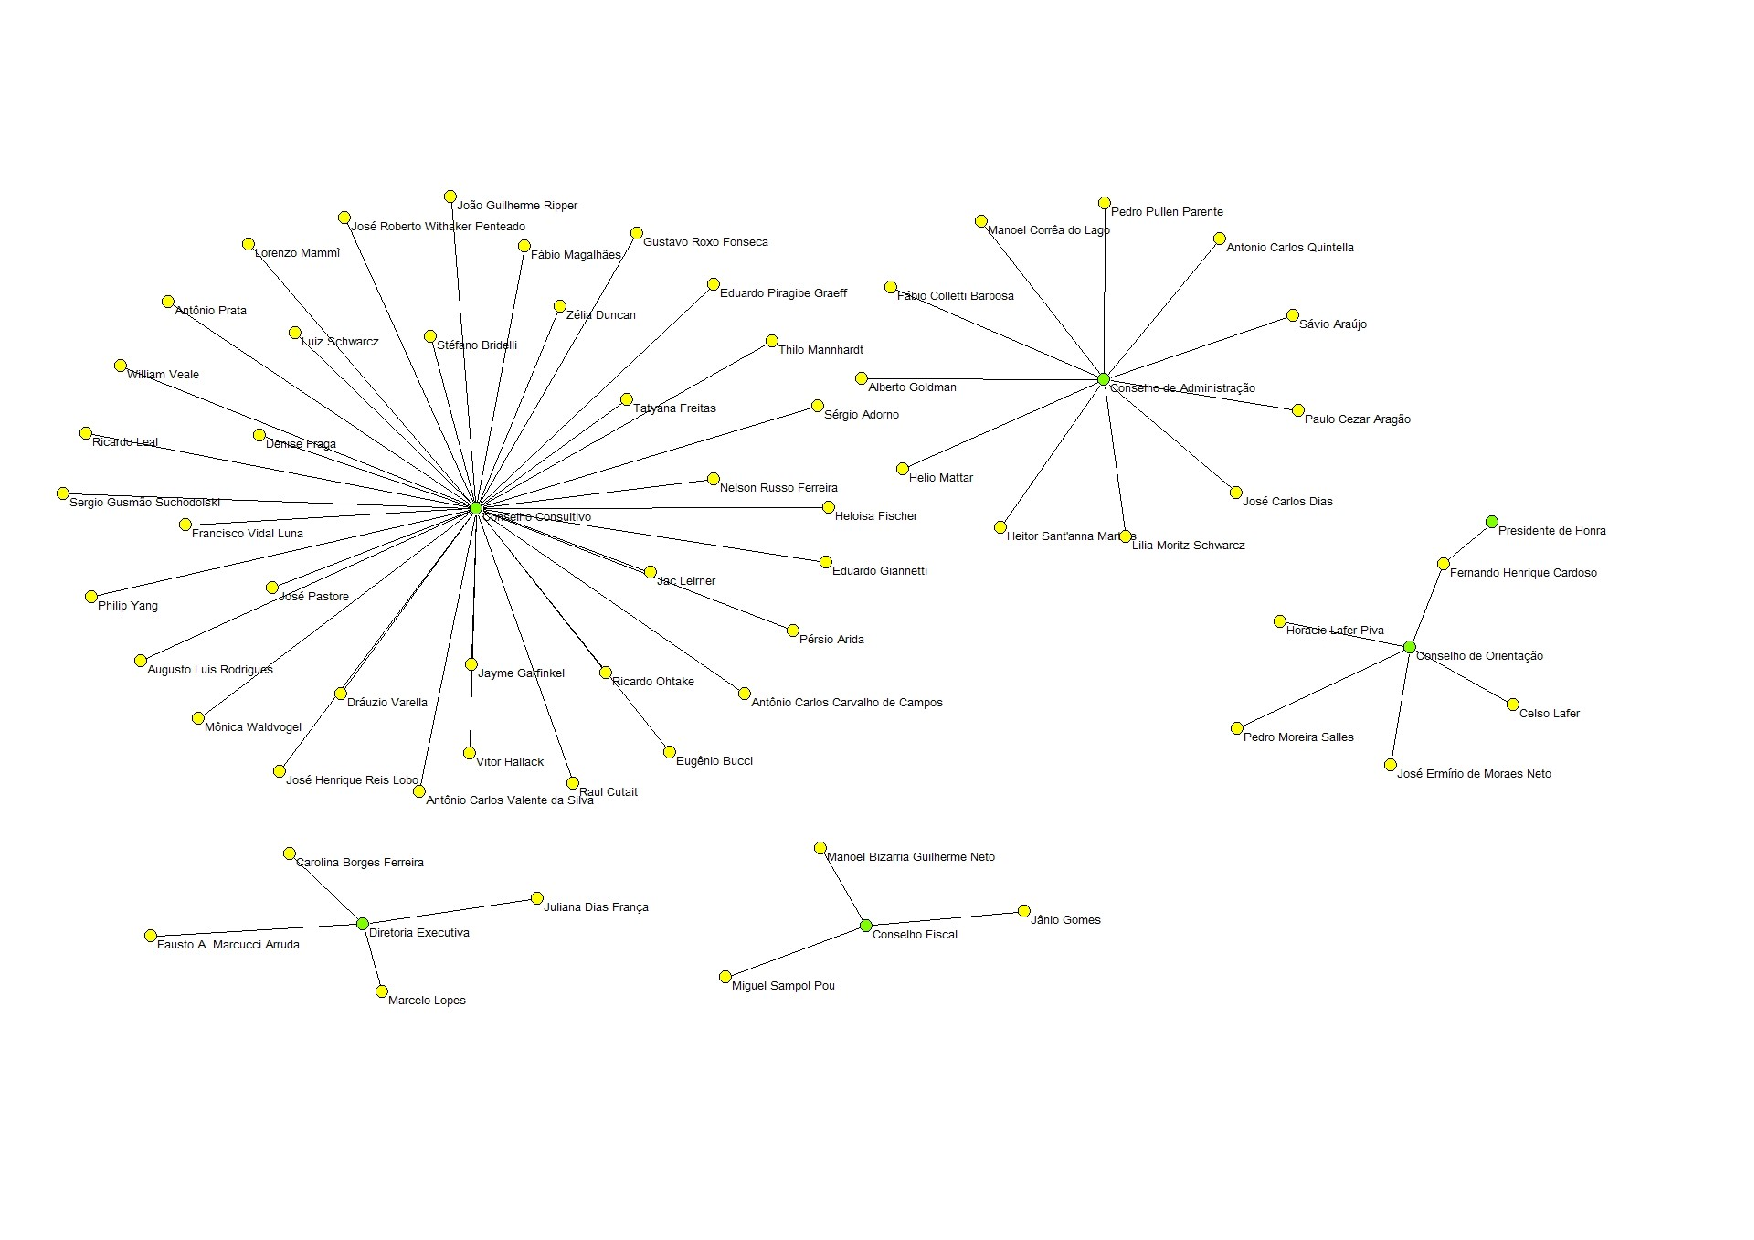
\includegraphics[scale=0.8]{OSESP_conselhos_pajek.pdf}

		\fonte{Site da \citeonline{osesp2016site}. Dados trabalhados pelo autor.}

	\end{sidewaysfigure}



	Além dos órgãos supracitados, a Fundação OSESP contém em sua base setores artísticos, pedagógicos e administrativos. São eles a Diretoria Artística, a Orquestra, o Coro, a coordenação artístico-pedagógica do Festival de Inverno de Campos do Jordão (festival de cunho formativo mantido pela Fundação OSESP), departamento jurídico, o Centro de Documentação Musical e Editora Criadores do Brasil, o setor de Atividades Educacionais (responsável pela Academia da Osesp, máster-classes e demais projetos formativos), departamento de marketing, departamento de comunicação, controladoria, contabilidade, departamento financeiro, uma divisão administrativa (composta de gerência, recepção, serviços de copa, serviços terceirizados, recursos humanos, informática, almoxarifado e arquivo), e uma divisão operacional (composta de departamento de produção, departamento técnico, iluminação, som, montagem, departamento de operações, controlador de acesso e indicadores). Essa estrutura está representada na Figura 6.



	\begin{sidewaysfigure}

		\centering

		\caption{A estrutura da Fundação OSESP 2}

		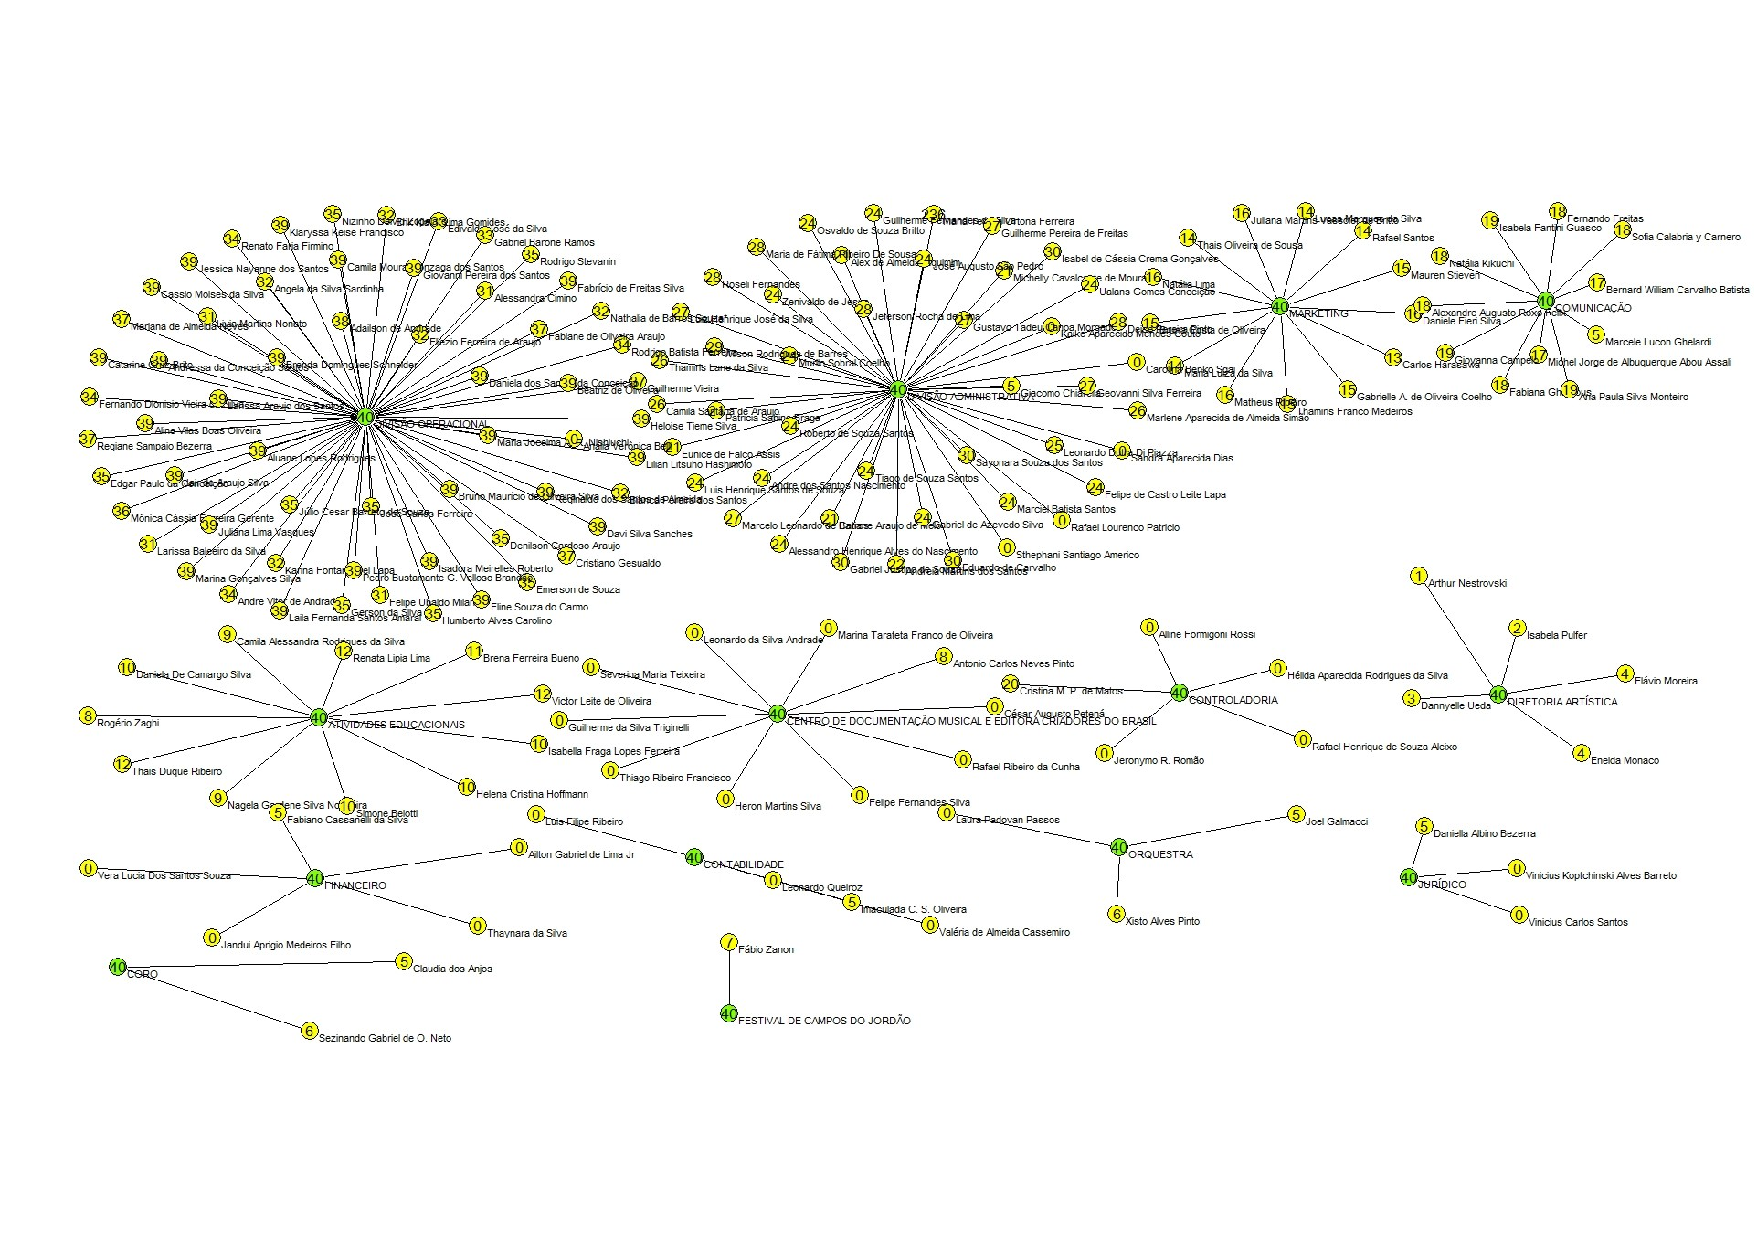
\includegraphics[scale=0.8]{OSESP_setores_pajek.pdf}

		\fonte{Site da \citeonline{osesp2016site}. Dados trabalhados pelo autor.}

	\end{sidewaysfigure}



	\subsection{Financiamento}



	Os recursos da OSESP provém de fontes diversificadas mas, sobretudo, diretamente do estado de São Paulo conforme o contrato de gestão vigente e, por outro lado, através da iniciativa privada. O Estado de São Paulo investiu, de 2010 a 2015 o montante de R\$251.676.666,67 distribuídos da seguinte forma: R\$7.166.666,67 em 2010, R\$43.400.000,00 em 2011, R\$53.400.000,00 em 2012, R\$55.500.000,00 em 2013, R\$55.650.000,00 em 2014 e R\$36.560.000,00 em 2015\footnote{O volume financeiro previsto para financiamento em 2015 a princípio era de R\$46.816.667,00 o qual foi alterado conforme o 6º termo de aditamento.}.



	Em 2014 (dados mais recentes publicados), a OSESP teve um custo total aproximado de R\$100.327.000,00 e uma receita total aproximada de R\$102.339.000,00. A distribuição das receitas por suas fontes estão apresentadas na tabela TAL.



	\begin{table}[ht]

		\IBGEtab{

			\centering

			\caption{Distribuição das porcentagens de financiamento da OSESP}

		}

		{\begin{tabular}{rrr}

				\hline

				& Fonte & (\%)\\

				\hline

				1 & Projetos Incentivados & 35 \\

				2 & Locação -- Eventos e Espaços & 18 \\

				3 & Assinatura e Bilheteria & 18 \\

				4 & Receitas Financeiras & 15 \\

				5 & Permutas e Patrocínios & 11 \\

				6 & Venda de Concertos & 3 \\

				7 & Outras Receitas Próprias & 0 \\

				\hline

			\end{tabular}

		}

		{\fonte{Elaboração do autor a partir de \citeonline{osesp2014compromisso}.}}

	\end{table}



	Em 2014 a OSESP captou R\$18.190.000,00 junto à iniciativa privada (mediante isenção fiscal) e R\$15.548.000,00 em mídia por meio de permutas. As empresas financiadoras da OSESP estão divididas em 3 categorias conforme o volume de recursos investidos: patrocinadores (valores acima de R\$500.000,00), apoiadores (valores acima de R\%200.000,00)  e outros apoiadores (cf. Figura TAL). O Programa Sua Orquestra, programa de financiamento voltado à captação de recursos junto à pessoas físicas, reuniu 654 associados e arrecadou um montante de R\$980.000,00.



	\begin{figure}[!ht]

		\centering

		\caption{Os investidores da OSESP em 2014}

		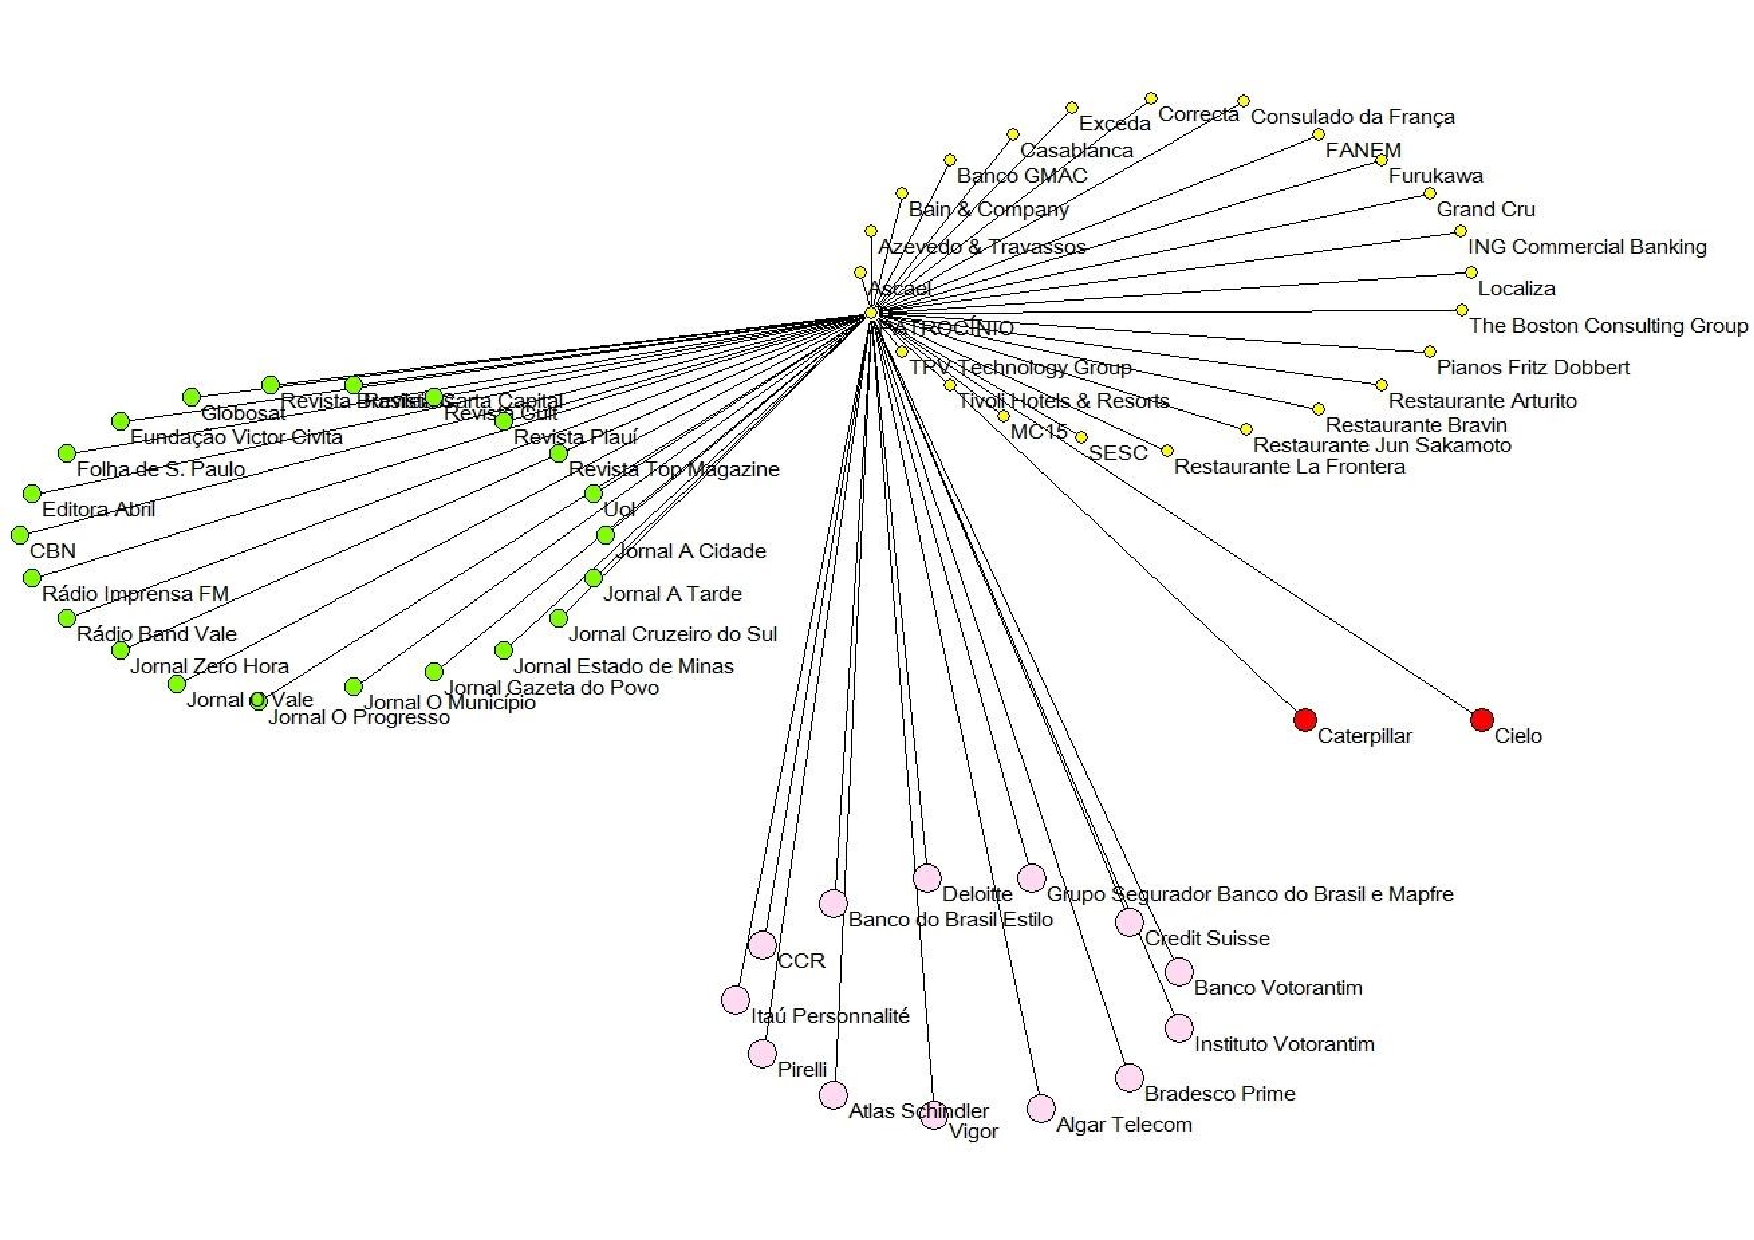
\includegraphics[scale=0.55]{OSESP_patrocinio.pdf}

		\fonte{Elaboração do autor a partir de \citeonline{osesp2014compromisso}.}

		\nota{Vértices rosas são patrocinadores, vermelhos são apoiadores, amarelos são outros apoiadores e verdes são veículos de comunicação parceiros via permuta. Com a exceção do grupo verde, o tamanho dos vértices indica as categorias de volume de investimento.}

	\end{figure}









	% Parei aqui!!!!!!!!!!

	%=================================================================

	%=================================================================

	\end{comment}

























	\chapter{O Campo}

	

	Criada muito recentemente, em 2008, a Orquestra Filarmônica de MG tem sido aclamada pela crítica nacional pela qualidade técnica e artística de suas apresentações. A organização pode ser divida em dois grandes setores: a orquestra propriamente dita e sua instituição mantenedora, o Instituto Cultural Filarmônica. A orquestra é composta por cerca de noventa músicos, o maestro e seu assistente, um gerente, um inspetor, um assistente administrativo, quatro arquivistas e seis montadores. Já o Instituto Cultural Filarmônica é formado pela Assembleia de Associados, pelo seu Conselho Administrativo, pela Diretoria Executiva, Equipe Técnica e Equipe Administrativa.



	A Diretoria Executiva do Instituto é formada pelo Diretor Presidente, pelo Diretor Administrativo-financeiro, pela Diretora de Comunicação, pela Diretora de MKT e Projetos, pelo Diretor de Operações e pelo Diretor de Produção Musical. A equipe técnica é formada pelo Gerente de Comunicação, Gerente de Produção Musical, Assessor de Programação Musical, Produtores, Analistas de Comunicação, Analista de MKT de Relacionamento, Analistas de MKT e Projetos, Assistente de MKT de Relacionamento, Assistente de Procução e quatro profissionais alocados na Sala Minas Gerais (Gerente de Infraestrutura, Gerente de Operações, Assistente Operacional e Técnico de Iluminação e Áudio). A equipe administrativa é formada pelo Gerente Administrativo-financeiro, Gerente de Recursos Humanos, Analistas Administrativos, Analista Contábil, Secretária Executiva, Assistente Administrativa, Assistente de Recursos Humanos, Recepcionista, Auxiliar Administrativo, Auxiliares de Serviços Gerais, Mensageiros e um menor aprendiz.



	%\begin{figure}[h]

	%	\centering

	%	\caption{Organograma da Orquestra Filarmônica de MG e do Instituto Cultural Filarmônica}

		%\includegraphics[keyvals]{imagefile}

	%	\fonte{Elaboração do autor a partir de dados disponíveis online}

	%\end{figure}



	Em seu funcionamento, ambos os setores se envolvem em relações comerciais ou artísticas com outros atores. No caso da orquestra, é comum a visita de solistas e maestros convidados. No caso do Instituto, uma rede de fornecedores nos mostra o âmbito dos recursos necessários à mobilização. Dentre os fornecedores do Instituto há assessoria contábil, assessoria jurídica, assessoria de imprensa, assessoria em TI, \textit{clipping}, criação e finalização de som, fotógrafos, gestão de projetos culturais, gráfica rápida, impressão digital, produção audiovisual, produção gráfica, sistema de assinaturas e compra de ingressos, serviços de segurança eletrônica, sistema de gestão e a redação de notas para os programas dos concertos.



	%\begin{sidewaysfigure}[!ht]

	%	\centering

	%	\caption{O Instituto Cultural Filarmônica e os recursos mobilizados}

	%	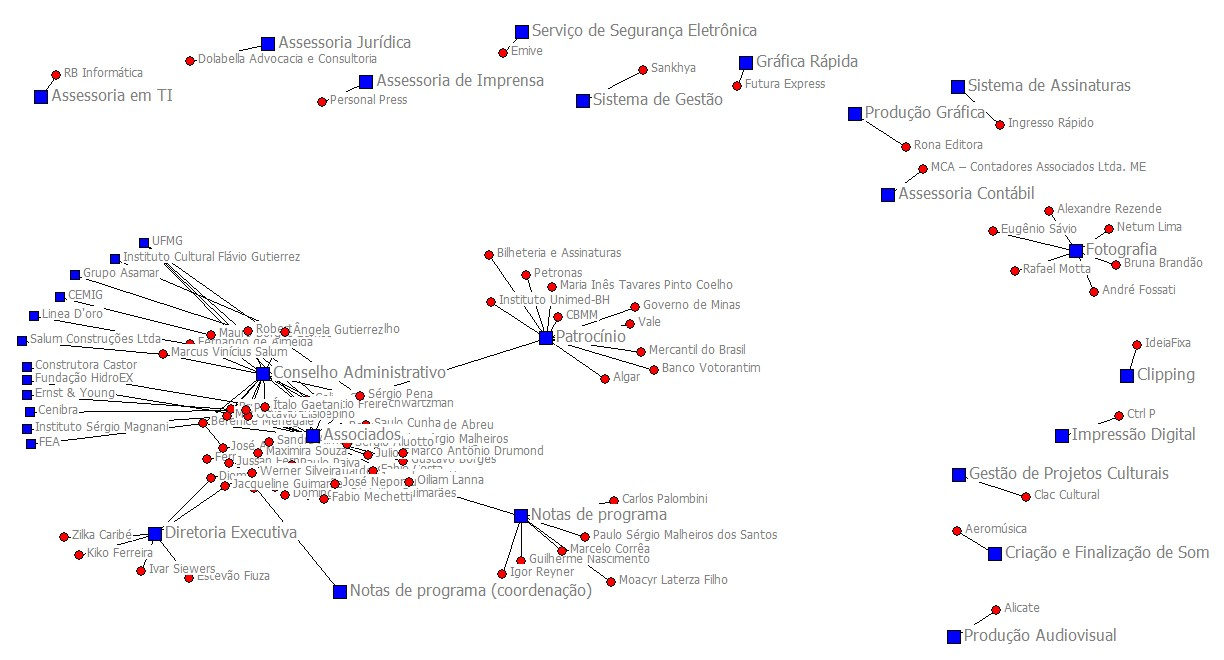
\includegraphics[scale=0.5]{filarmonica_rede2mode.eps}

	%	\fonte{Elaboração do autor com dados disponíveis online \cite{filarmonica2015site}.}

	%	\label{fil2mode}

	%\end{sidewaysfigure}



	É possível perceber a complexidade da teia de recursos que o Instituto mobiliza no decurso de suas atividades cotidianas. Além dos serviços de caráter administrativo como assessorias contábil, jurídica, de TI e outros serviços comuns no campo da cultura como gráfica rápida, fotografia e assessoria de imprensa, é curioso notar alguns serviços que parecem peculiares (embora não exclusivos) ao universo da orquestra. A redação das notas de programa é feita por professores de universidades públicas e pesquisadores vinculados a programas de pós-graduação no exterior. Essas notas de programa geralmente funcionam como um guia ao ouvinte e são inseridas no ``Fortíssimo'', uma publicação mensal da orquestra contendo ainda as biografias dos maestros e solistas convidados e notícias da orquestra. Mais do que um simples programa de concertos, o ``Fortíssimo'' é uma publicação indexada em sistemas nacionais e internacionais de catalogação. As notas de concerto geralmente informam o expectador sobre alguns pontos importantes da biografia do compositor, algumas questões estéticas e estilísticas envolvendo a obra programada para execução além de algumas sugestões de escuta da obra e leitura relacionada. A publicação é distribuída gratuitamente e, ao fim dos concertos, os ouvintes tem a oportunidade de retorná-la, caso não queiram guardá-la.



	O Instituto também mantém uma relação comercial com uma empresa especializada em gestão de projetos culturais. Isso faz sentido se sabemos que uma boa fatia dos recursos captados pela orquestra o são mediante projetos de isenção fiscal.



	\subsection{Recursos Financeiros}



	A Orquestra Filarmônica conta em 2015 com um financiamento de R\$22.348.993,00 proveniente de fontes diversificadas. A instituição recebe fundos direto do Governo de Minas, seu principal financiador, de empresas investidoras através de leis de incentivo à cultura e do público pagante.



	%\begin{figure}[t]

	%	\begin{center}



	%		\caption{Os financiadores da Filarmônica}

	%		\begin{center}

	%			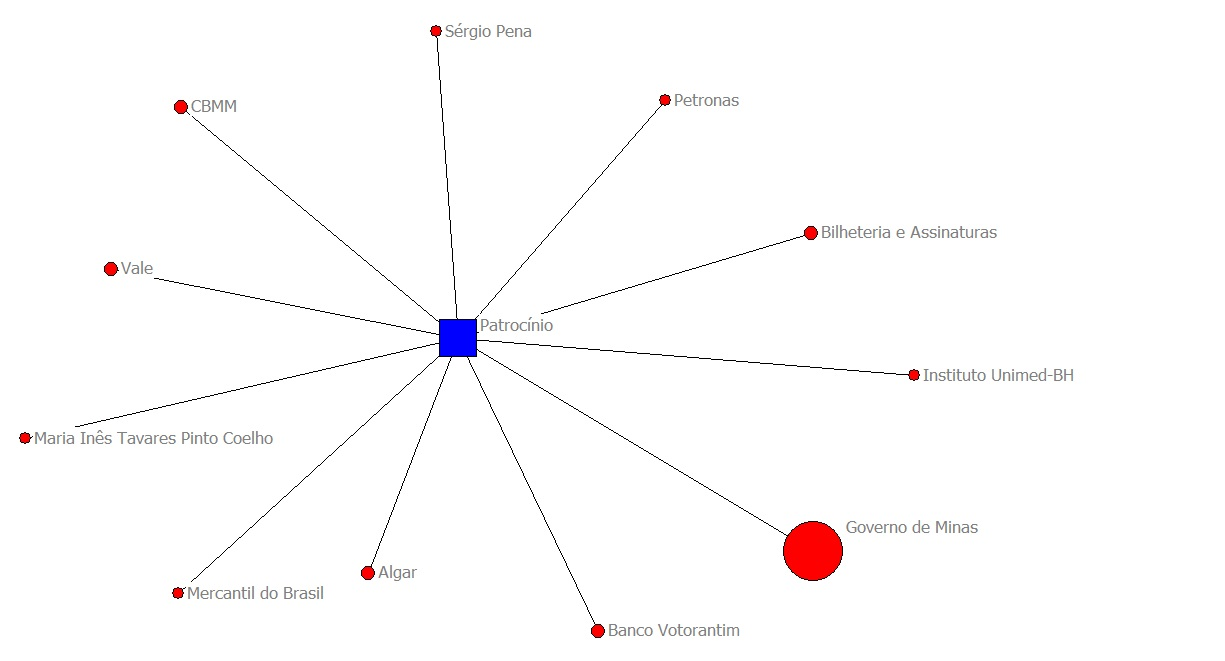
\includegraphics[scale=0.6]{filarmonica_patrocinadores.eps}

	%		\end{center}

	%		\fonte{Elaboração do autor a partir de \citeonline[p. 13]{minas2015} e \citeonline[p. 23-4]{filarmonica2015gerencial}. Os tamanhos dos vértices no grafo indicam o volume de capital investido na instituição.}

	%	\end{center}

	%\end{figure}



	Seu maior financiador, o Governo de Minas é responsável por 81,69\% de seu financiamento total.



	% latex table generated in R 3.2.1 by xtable 1.7-4 package

	% Thu Oct 15 01:17:07 2015

	\begin{table}[ht]
		\IBGEtab{
			\centering
			\caption{Fontes de financiamento da Filarmônica em 2015}
		}
		{\begin{tabular}{rrrrc}
				\hline
				& Fontes & Montantes (R\$) & (\%) & \% acumulada \\
				\hline
				1 & Algar & 595.400,00 & 2.66 & 2.66 \\
				2 & Banco Votorantim & 900.000,00 & 4.03 & 6.69 \\
				3 & Bilheteria e Assinaturas & 736.312,82 & 3.29 & 9.99 \\
				4 & CBMM & 500.000,00 & 2.24 & 12.22 \\
				5 & Governo de Minas & 18.257.024,50 & 81.69 & 93.91 \\
				6 & Instituto Unimed-BH & 299.955,68 & 1.34 & 95.26 \\
				7 & Maria Inês Tavares Pinto & 300,00 & 0.001 & 95.26 \\
				8 & Mercantil do Brasil & 207.000,00 & 0.93 & 96.18 \\
				9 & Petronas & 150.000,00 & 0.67 & 96.85 \\
				10 & Sérgio Pena & 3.000,00 & 0.01 & 96.87 \\
				11 & Vale & 700.000,00 & 3.13 & 100.00 \\
				\hline
				& TOTAL & 22.348.993,00 &  & \\
				\hline
			\end{tabular}
		}
		{\fonte{Elaboração do autor a partir de \citeonline[p. 13]{minas2015} e \citeonline[p. 23-4]{filarmonica2015gerencial}.}
		}
	\end{table}



	Fica claro o papel decisivo do Estado como mantenedor da Orquestra Filarmônica de MG. Sem mais de 80\% de seu orçamento anual imaginamos que seria bastante difícil para os dirigentes manterem a cota de concertos e os convites a maestros e solistas convidados. 3.3\% do orçamento provém do pagamento de ingressos e assinaturas. Em termos absolutos, o valor representa uma quantia vultuosa se comparado ao campo cultural de um modo geral. Entretanto, representa uma pequena fatia no financiamento da orquestra.



	O restante do financiamento da instituição vem de empresas privadas por meio do mecanismo de incentivo fiscal das leis de incentivo à cultural federal e estadual. Na modalidade de incentivo fiscal, a lei federal (Rouanet) concede às empresas financiadoras de cultura no Brasil uma porcentagem de desconto no Imposto de Renda (IR). A lei estadual de Minas Gerais concede desconto no Imposto sobre Circulação de Mercadorias e Serviços (ICMS). O volume de financiamento adquirido via lei Rouanet corresponde a 12,35\% do total enquanto aquele adquirido via lei estadual, 2,66\% (apenas a empresa Algar patrocina por esse meio). Curioso notar que, apesar de as empresas constarem como financiadoras da orquestra, de fato o dinheiro investido provem de isenção fiscal, portanto, dinheiro público. Mesmo os investimentos feitos por pessoas físicas (dois casos) também acontecem mediante isenção fiscal. O Estado aparece aqui como um grande centralizador do financiamento da orquestra.


	
	\section{A Filarmônica de MG}
	
	%Minas Gerais Philharmonic Orchestra began its activities in 2008 led by maestro Fabio Mechetti. It was created from a partnership between Minas Gerais State and \textit{Instituto Cultural Filarmônica}, the maintainer of the orchestra. ``\textit{Instituto Cultural Filarmônica} is a non-profit civil association that has the goals of structuring and maintaining Minas Gerais Philharmonic and promote the diffusion of classical music''\footnote{\fonte{Minas Gerais Philharmonic Website, \url{http://www.filarmonica.art.br/instituto/instituto-cultural-filarmonica/}.}}.
	%The recognition of the \textit{Instituto Cultural Filarmônica} as an \textit{OSCIP}, an Organization of the Civil Society of Public Interest grants them the possibility of signing partnership contracts \cite{minas2017aditivo} with State Government and, therefore, receive investments directly from it. This partnership contract states the amount of resources invested by the government as well as both parts' duties. The document also states the goals and the criteria by which the contract and the orchestra will be evaluated. Those criteria are particularly interesting to us specially because they indicate the weights with which the state conceives artistic quality. Those criteria are divided in 8 large groups and disaggregated according to Table \ref{goals} \cite{filarmonica2017gerencial}:
	
	A Orquestra Filarmônica de Minas Gerais iniciou suas atividades em 2008 liderados pelo maestro Fabio Mechetti. Ela foi criada em uma parceria entre o Governo do Estado de Minas Gerais e o Instituto Cultural Filarmônica, a mantenedora da orquestra. ``O Instituto Cultural Filarmônica é uma associação civil sem fins lucrativos que tem como tarefas estruturar e manter a Orquestra Filarmônica de Minas Gerais e promover a difusão da música clássica'' \footnote{Fonte: Site da Orquestra Filarmônica de Minas Gerais, \url{http://www.filarmonica.art.br/instituto/instituto-cultural-filarmonica/}.}. O reconhecimento do Instituto como uma OSCIP, uma Organização da Sociedade Civil de Interesse Público dá a ele a possibilidade de assinar contratos de parceria \cite{minas2017aditivo} com o Governo do Estado e, portanto, receber investimentos diretamente dele. Esse contrato de parceria estabelece o volume de recursos investido pelo governo bem como os direitos e deveres de ambas as partes. O documento também estabelece os objetivos e os critérios pelos quais o contrato e a orquestra serão avaliados. Esses critérios são particularmente interessantes para nós especialmente porque eles indicam os pesos com os quais o Estado concebe qualidade artística.  Esses critérios estão divididos em oito grandes grupos conforme a Tabela \ref{goals} \cite{filarmonica2017gerencial}:
	
	
	
	
	
	\begin{table}[!h]
		\ibgetab{
			\centering
			\caption{Objetivos da Orquestra}
			\label{goals}
		}
		{\begin{tabular}{p{6cm} p{7cm} c}
				\hline
				\textbf{Grupo}  & \textbf{Objetivo} & \textbf{Peso} \\
				\hline
				Execução de concertos de assinatura & Número cumulativo de concertos sinfônicos de assinatura no ano de referência & 15 \\
				& Percentual médio de ocupação dos concertos de assinatura de Quinta & 4 \\
				& Percentual médio de ocupação dos concertos de assinatura de Sexta & 4 \\
				& Percentual médio de ocupação dos concertos de assinatura de Sábado & 4 \\
				& Número de assinaturas para séries de concertos sinfônicos & 3 \\
				& Taxa de renovação de assinaturas em relação ao ano anterior & 3 \\
				\hline
				Educação e formação de público para música & Número cumulativo de concertos da série Concertos para a Juventude & 5 \\
				& Percentual médio de ocupação da série Concertos para a Juventude & 4 \\
				& Número cumulativo de concertos da série Concertos Didáticos & 0.5 \\
				& Percentual médio de ocupação da série Concertos Didáticos & 0.5 \\
				& Número cumulativo de concertos da série Música de Câmara & 0.5 \\
				& Percentual médio de ocupação da série Música de Câmara & 0.5 \\
				\hline
				Democratização do acesso à música clássica & Número cumulativo de concertos em praças públicas ou parques na região metropolitana de Belo Horizonte & 0.5 \\
				& Número médio de pessoas nos concertos em praças públicas ou parques da região metropolitana de Belo Horizonte & 0.5 \\
				& Número cumulativo de concertos fora de Belo Horizonte e dentro de Minas Gerais & 0.5 \\
				& Percentual médio de ocupação dos concertos fora de Belo Horizonte e dentro de Minas Gerais & 0.5 \\
				\hline
				Representar o Estado de Minas Gerais nacionalmente e internacionalmente & Número de concertos fora de Minas Gerais & 0.5 \\
				& Percentual médio de opcupação dos concertos fora de Minas Gerais & 0.5 \\
				\hline
				Estímulo à revelação de novos talentos para a música clássica & Realização do \textit{Laboratório de Regência} e o \textit{Festival Tinta Fresca} & 5 \\
				& Percentual médio de ocupação do \textit{Laboratório de Regência} e do \textit{Festival Tinta Fresca} & 4 \\
				\hline
				Prover novas experiências e conhecimento ao corpo arstítico da orquestra & Número cumulativo de regentes convidados e solistas convidados & 5 \\
				\hline
				Financiamento & Financiamento através da bilheteria e assinaturas & 10 \\
				& Financiamento através de patrocínios & 10 \\
				& Dependência dos fundos do contrato de parceria & 10 \\
				\hline
				Gestão da parceria & Percentual de acordo das peças de comunicação da Filarmônica com as direções da OEP & 3 \\
				& Acordo dos processos analisados na chegagem períodica amostral & 3 \\
				& Efetividade do monitoramento do contrato de parceria & 3 \\
				\hline
				
			\end{tabular}
		}
		{\fonte{\cite[p. 3-4]{filarmonica2017gerencial}}}
	\end{table}
	
	
	%It is very interesting to notice that if we observe the disaggregated goals, the one with the greatest weight is the cumulative number of signature symphonic concerts but if we observe the groups, the one with the greatest weight is Fund-raising. The signature symphonic concerts are the main activity of the orchestra, the concerts with the most challenging repertoire and that receive the most prestigious guests conductors and soloists. On the other hand, fund-raising states for the management capacities of the maintainer, its capability of running a sustainable of even profitable business.
	
	É muito interessante notar que se observarmos os objetivos desagregados, aquele que possui o maior peso é o número cumulativo de concertos sinfônicos realizados. Entretanto, observando os grupos, o grupo com maior peso é o Financiamento. Os concertos sinfônicos de assinatura são a principal atividade da orquestra. São concertos com o repertório mais desafiador e que recebem os maestros e solistas convidados de maior prestígio. Por outro lado, o grupo de Financiamento se relaciona com as capacidades de gestão da mantenedora, sua capacidade de gerir um negócio sustentável e, até mesmo, lucrativo.
	
	Examinaresmos agora os objetivos da orquestra em maiores detalhes.
	
	\subsection{Avaliação dos objetivos da orquestra}
	
	%The first goal group is evaluated regarding the total number of concerts presented in a season, regarding the occupancy of these concerts and regarding the number of signatures\footnote{In Brazil, a signature is a ticket set for all the concerts within a specific series. They can be bought just for a specific series, for combinations of series or for all the concerts in a season.} sold and renewed. The total number of concerts is essentially a quantitative measure of the orchestra's supply. The average percentage of occupancy can be understood, according to the reviewed literature, as a qualitative measure of the concerts. The number of signatures sold and renewed can be understood both as a measure of quality and as a measure of the management capacity of the organization. 
	
	O primeiro grupo de objetivos é avaliado com relação ao número total de concertos apresentados em uma temporada, com relação à ocupação desses concertos e com relação ao número de assinaturas\footnote{Uma assinatura é um conjunto de ingressos para todos os concertos de uma série específica. Eles podem ser comprados apenas para uma série, para uma combinação de séries ou para todos os concertos da temporada.} vendidas e renovadas. O número total de concertos é essencialmente uma medida quantidade da produção da orquestra. O percentual médio de ocupação pode ser entendido, de acordo com a literatura revisada, como uma medida qualitativa dos concertos. O número de assinaturas vendidas e renovadas pode ser entendido tanto quanto uma medida de qualidade quanto uma medida da capacidade gerencial da organização.
	
	%The second group of goals (Education and Formation of Public) is evaluated mainly through one concert series, \textit{Concertos para a Juventude} (Youth concerts). These concerts usually take place on Sunday mornings with low ticket prices and are destined to formation of public. They present ``accessible language to the diffusion of the repertoire of orchestral music'' \cite[p. 9]{filarmonica2017gerencial}. The number of Youth concerts offered and the average percentage of occupancy are the main measures to evaluate this group. The other series that are part of this strategy, the Didactic concerts\footnote{Concerts exclusive to students of the public education system, children's groups social institutions and universities.} and the Chamber concerts\footnote{Concerts with smaller formations, usually string quartets, brass quintets, wood quintets, string trio and piano, etc.} have a very low weight (0.5).
	
	O segundo grupo de objetivos (Educação e Formação de Público) é avaliado principalmente através de uma série de concertos, os Concertos para a Juventude. Esses concertos usualmente acontecem no Domingo pela manhã com ingressos a preços baixos e são destinados à formação de público. Eles apresentam ``linguagem acessível para a difusão do repertório da música orquestral'' \cite[p. 9]{filarmonica2017gerencial}. O número de Concertos para a Juventude realizados e o percentual médio de ocupação são as principais métricas para avaliar esse grupo. As outras séries que fazem parte dessa estratégia, os Concertos Didáticos\footnote{Concertos exclusivos para estudantes da rede pública de ensino, grupos de crianças, instituições sociais e universidades.} e os concertos de Câmara\footnote{Concertos com formações menores, usualmente quartetos de cordas, quintetos de metais, quintetos de madeiras, trio de cordas com piano, etc.} tem um peso mais baixo (0.5).
	
	%The third and fourth groups of goals have a very low impact on the evaluation. These groups are related to orchestra trips to outside the capital of Minas Gerais, to other states and abroad.
	
	O terceiro e o quarto grupos de objetivos tem um impacto baixo na avaliação. Esses grupos são relacionados às viagens da orquestra para fora da capital mineira, outros estados e ao exterior.
	
	%The fifth group is evaluated by the \textit{Laboratório de Regência} (Conducting Lab) and the \textit{Tinta Fresca} Festival. The first event is a conducting masterclass with the orchestra under the guidance of maestro Fabio Mechetti. Nineteen students are selected to participate, fifteen as listener students and four as fully participating students. Those students spend three to four days working with the orchestra on a given repertoire and, at the end, they conduct a concert. The second event is an award to new compositions. The first place winner receives a prize and his composition is included in the next season schedule.
	
	O quinto grupo é avaliado pelo \textit{Laboratório de Regência} e pelo \textit{Festival Tinta Fresca}. O primeiro evento consiste de uma masterclasse de regência com a orquestra sob a orientação do maestro Fabio Mechetti. Dezenove estudantes são selecionados para participar, quinze como ouvintes e quatro como alunos executantes (ou ativos). Estes alunos passam de três a quatro dias trabalhando com a orquestra em um dado repertório e, ao fim, conduzem o concerto de encerramento. O segundo evento consiste de um prêmio para novas composições. O vencedor, além do prêmio, tem sua composição incluída no repertório da temporada seguinte.
	
	%The sixth group is evaluated by a single goal, which is the number of guest conductors and soloists. The partnership contract defines guests conductors as ``Those who do not have permanent contract or employment relationship with the orchestra but come to conduct it or a lyric chorus by invitation of the maintainer'' \cite[p. 40]{minas2017aditivo} and guest soloists as ``instrumentalists or singers who do not have permanent contract or employment relationship with the orchestra and participate on concerts by invitation of the maintainer, playing pieces that require their individual participation'' \cite[p. 40]{minas2017aditivo}. Eventually, musicians that have permanent contract with the orchestra and stand out in the classical music field can be invited to play as a guest soloist.
	
	O sexto grupo é avaliado por um único objetivo, qual seja, o número de regentes e solistas convidados na temporada. O contrato de parceria define regentes convidados como ``Aqueles que não possuem contrato permanente ou vínculo empregatício com a orquestra mas que vem conduzi-la ou o coral lírico por convite da mantenedora'' \cite[p. 40]{minas2017aditivo} e solistas convidados como ``instrumentistas ou cantores que não possuem contrato permanente ou vínculo empregatício com a orquestra e participam de concertos por convite da mantenedora, tocando peças que requerem sua participação individual''  \cite[p. 40]{minas2017aditivo}. Eventualmente, músicos que possuem contrato permanente com a orquestra e se destacam no cenário da música clássica podem ser convidados a se apresentarem como solistas convidados.
	
	%The seventh group, Fund-raising, has the biggest impact on the orchestra evaluation by the State. This group is evaluated by fund-raising through the box office and signatures sold, fund-raising through sponsorship and the ``Dependency on the partnership contract'' score. The first and the second goals are measured in Brazilian Reais (R\$) and the third one is given by a ratio between budget from the partnership contract over total budget.
	
	O sétimo grupo, Financiamento, tem o maior impacto na avaliação da orquestra pelo Estado. Este grupo é avaliado pelo financiamento proveniente da bilheteria e assinaturas vendidas, pelo financiamento através de patrocínio e pela medida de ``Dependência do contrato de parceria''. O primeiro e segundo objetivos são mensurados em reais brasileiros (R\$). O terceiro é definido por uma razão entre o orçamento do contrato de parceria sobre o orçamento total.
	
	%The eighth and last group regards the management of the partnership contract and is evaluated by technical directions regarding marketing material, bureaucratic processes and the monitoring of the contract. We will now take a look at some of this goals in a deeper way.
	
	O oitavo e último grupo está relacionado com a gestão do contrato de parceria e é avaliado por direcionamentos técnicos com relação ao material de marketing, processos burocráticos e monitoramento do contrato. Observaremos agora alguns dos objetivos de maneira mais aprofundada.
	
	\subsection{Principais concertos}
	
	%The ``signature concerts'' are composed by the series called \textit{Allegro}, \textit{Vivace}, \textit{Veloce}, \textit{Presto} and \textit{Fora de Série}. Allegro's concerts happen on thursdays and privilege Romantic and beginning of 20th century repertoire. These concerts are repeated on fridays with the name Vivace. The same logic operates on Presto (thursdays) and Veloce (fridays) concerts. \textit{Fora de Série}'s concerts happen on saturdays and they follow a theme chosen for the season. For instance, 2015's theme was Beethoven, 2016's theme was Mozart, 2017's was Baroque Music and 2018's theme was ``Expeditions'', music from around the globe.
	
	Os ``concertos de assinatura'' são compostos pelas séries chamadas \textit{Allegro}, \textit{Vivace}, \textit{Veloce}, \textit{Presto} and \textit{Fora de Série}. Os concertos da série Allegro acontecem às quintas e privilegiam repertório Romântico e do início do século XX. Esses concertos são repetidos às sextas com o nome Vivace. A mesma lógica opera nos concertos da série Presto (quintas) e Veloce (sexta). Concertos da série \textit{Fora de Série} acontecem aos sábados e normalmente seguem uma temática escolhida para a temporada. Por exemplo, em 2015 o tema escolhido foi Beethoven, em 2016, Mozart, em 2017 música barroca e em 2018 ``Expedições'', música ao redor do mundo.
	
	%Those are the main products of the orchestra, the ones by which it gains its prestige, its status. Also, these concerts are responsible for the biggest part of the orchestras income (.....) %%% MOSTRAR EM UM GRÁFICO.
	
	Estes são os principais produtos da orquestra, aqueles pelos quais ela ganha o seu prestígio, seu status. Além disso, esses concertos são responsáveis pela maior parte das receitas da organização. (.....)  MOSTRAR EM GRÁFICO......
	
	
	
	\subsection{Financiamento e dependência do Estado}
	
	%Although one of the most important criteria chosen by the state to evaluate the orchestra is related to its capacity of sustainability, that is, the orchestra's capacity of raising funds from outside the direct investment of the partnership contract, it does not constrain the orchestra to any expectations of less dependency on the State itself. The most part of the investment from private companies is really public money because it is obtained through the laws to encourage culture.
	
	Embora um dos critérios mais importantes escolhidos pelo Estado para avaliação da orquestra esteja relacionado com sua capacidade de ser sustentável, ou seja, sua capacidade de levantar fundos fora do investimento direto via contrato de parceria, ele não impõe sobre a orquestra nenhuma expectativa de menor dependência do Estado em si. A maior parte dos investimentos de companhias privadas é, de fato, dinheiro público visto que são obtidos através de leis de incentivo à cultura.
	
	PRESENT VALUES AND RATES................
	
	
	\subsection{Repertório e consumo}
	
	%Up to 2014, the orchestra held its main concerts at the \textit{Palácio das Artes} great hall. Usually, the concerts took place once a week or once in two weeks. In 2015, Minas Gerais Hall was inaugurated, a highly technological concert hall that hosts the main Minas Gerais Philharmonic concerts. Also, the opening of this new venue changed the orchestra's supply logic. Concerts began to happen in a weekly basis on thursdays and fridays (cf. ``main concerts'' section) and a new concert series was opened on saturdays.
	
	Até 2014, a orquestra apresentava seus principais concertos no Grande Teatro do Palácio das Artes. Usualmente os concertos aconteciam uma vez por semana ou uma vez a cada duas semanas. Em 2015 a Sala Minas Gerais foi inaugurada, uma sala de concertos altamente tecnológica que abriga os principais concertos da Filarmônica a partir desse ano. Além disso, a abertura da sala modificou a lógica de produção da orquestra. Os concertos passam a acontecer semanalmente às quintas, sextas e em alguns sábados.
		
	% APRESENTAR ALGUMAS ANÁLISES DE REPERTÓRIO, SAZONALIDADE, DIFERENÇA DE PÚBLICO, ETC......
	
	%For 2015 and 2016, 85\% of all the orchestras concerts happened at Minas Gerais Hall. As we can see in Figure \ref{repertoire-peryear}, the orchestra seems to privilege Romantic and Modern\footnote{Period coding was made by the author. Beethoven was always included in Romantic category. Modern category refers to music of the 20th century.} repertoire.
	
	Para 2015 e 2016, 85\% de todos os concertos da orquestra aconteceram na sala Minas Gerais. Como podemos observar na Figura \ref{repertoire-peryear}, a orquestra parece privilegiar repertório Romântico e Moderno\footnote{A codificação dos períodos de cada obra foi feita pelo autor. Beethoven sempre foi classificado como \textit{romântico}. A categoria \textit{moderno} se refere à música do séc XX.}.
	
	\begin{figure}[!h]
		\centering
		\caption{Repertório da orquestra}
		\label{repertoire-peryear}
		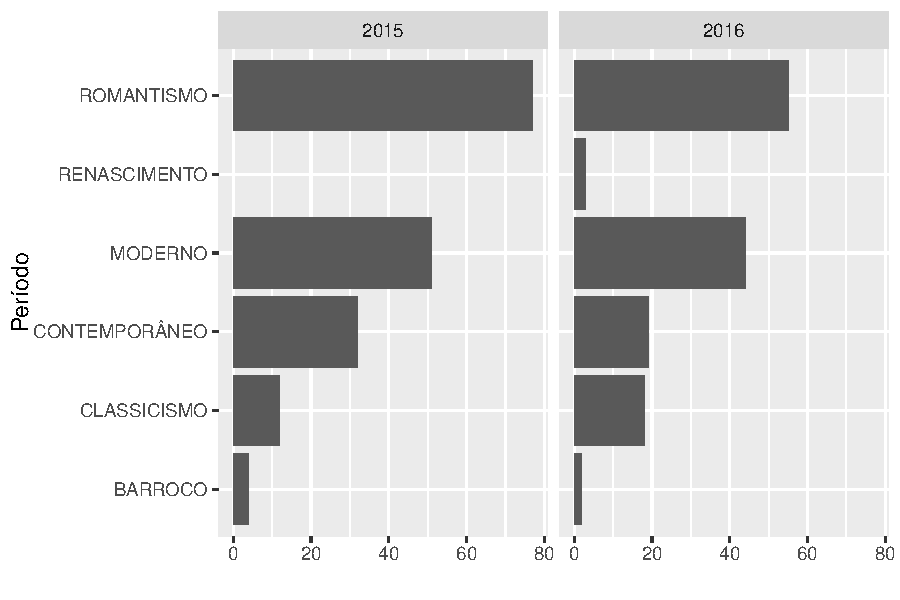
\includegraphics[scale=1]{periodo_peryear.pdf}
		\fonte{Elaborado pelo autor.}
	\end{figure}
	
	
	%This proportion stays somewhat stable if we observe the main concert series (with the exception, of course, of the \textit{Fora de Série} thematic series). In Figure \ref{repertoire-perseries}, the Youth Concerts (in the middle column) seems to be the most balanced series. Allegro/Vivace and Presto/Veloce seem quite alike. In 2016, less Classical music has been made in these series. The genre was reserved in that year to \textit{Fora de Série} concerts. 
	
	Essa proporção continua relativamente estável se observamos as principais séries de concertos (com exceção, é claro, da \textit{Fora de Série} que é temática). Na Figura \ref{repertoire-perseries}, os Concertos para a Juventude (na coluna central) parecem ser a série mais balanceada. Allegro/Vivace e Presto/Veloce possuem grande similaridade. Em 2016, menos repertório clássico foi feito nessas séries. O gênero ficou reservado naquele ano para a série \textit{Fora de Série}.
	
	\begin{figure}[!h]
		\centering
		\caption{Repertório por série}
		\label{repertoire-perseries}
		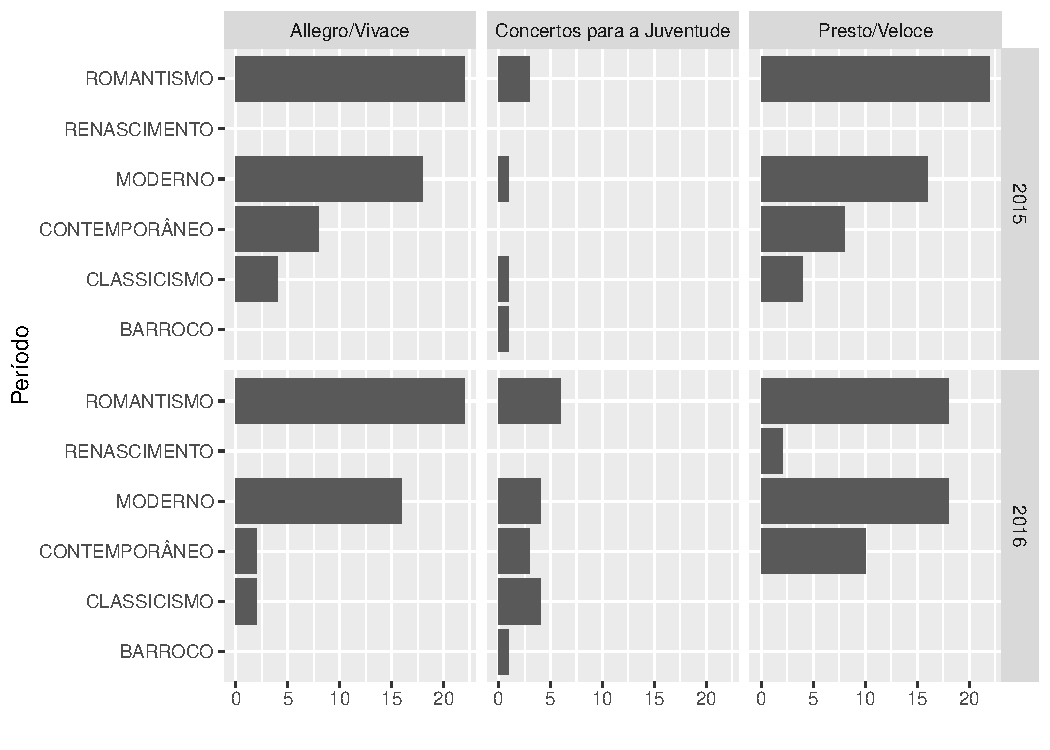
\includegraphics[scale=1]{periodo_perserie_year.pdf}
		\fonte{Elaborado pelo autor.}
	\end{figure}
	
	
	%In order to investigate the consumption, the 2016 results report gives us the number of seats available and the number of tickets sold to calculate the occupancy rate. At first, we are tented to believe that the consumption of the concerts is mostly related by the chosen repertoire which, therefore, would reflect on the concert series. Nevertheless, because of the change in the concerts offering since 2015, we believe that the weekday has a larger impact on consumption. Linear models showed that the series has a bigger explanatory power on consumption (cf. Table \ref{concert-consumption-models}). The models were estimated with the occupancy rate as the dependent variable and only for 2016\footnote{Unfortunately, the number of seats available is only reported in 2016's reports. In order to make our further analysis more robust, we estimated the seats available for 2015 given that the venues, the weekdays of the concerts and the series were the same as 2016. A technical description of the estimation procedure is given in the appendix.}.
	
	Para investigar o consumo, o relatório de resultados de 2016 da Filarmônica nos dá o número de assentos disponíveis e o número de ingressos vendidos para calcular a taxa de ocupação. Numa primeira análise, somos tentados a acreditar que o consumo de concertos está altamente relacionado com o repertório escolhido o qual, portanto, refletiria nas séries de concertos. Contudo, por causa da mudança na oferta dos concertos desde a inauguração da Sala Minas Gerais em 2015, acreditamos que o dia da semana tem maior impacto no consumo. Modelos lineares mostraram que as séries tem maior poder explicativo sobre sobre o consumo (cf. Tabela \ref{concert-consumption-models}). Os modelos foram estimados tendo Taxa de Ocupação como variável dependente e apenas usando dados de 2016\footnote{Infelizmente, o número de assentos disponíveis foi reportado apenas no relatório de 2016, não em 2015. Para realizarmos análises mais robustas, estimamos os assentos disponíveis em 2015 dado que os locais, séries e dia da semana eram os mesmos em 2016. Uma descrição técnica do processo de estimação é apresentada no apêndice.}.


	
	\begin{table}[!ht]
		\ibgetab{
			\centering
			\caption{Consumo de concertos - Modelos Lineares}
			\label{concert-consumption-models}
		}
		{\begin{tabular}{l c c }
				\hline
				& Modelo 1 & Modelo 2 \\
				\hline
				(Intercepto)                                        & $85.28^{***}$ & $93.36^{***}$  \\
				& $(1.84)$      & $(1.46)$       \\
				\textbf{Dia da semana} & & \\
				Domingo & $14.72^{***}$ &                \\
				& $(3.98)$      &                \\
				Quinta  & $4.59$        &                \\
				& $(2.58)$      &                \\
				Sábado  & $12.15^{***}$ &                \\
				& $(3.10)$      &                \\
				\textbf{Série de Concertos} & & \\
				Concertos para a Juventude                    &               & $6.64^{*}$     \\
				&               & $(3.21)$       \\
				Fora de Série                                 &               & $6.13^{*}$     \\
				&               & $(2.65)$       \\
				Presto/Veloce                                 &               & $-11.26^{***}$ \\
				&               & $(2.05)$       \\
				\hline
				R$^2$                                              & 0.28          & 0.53           \\
				Adj. R$^2$                                         & 0.25          & 0.50           \\
				Num. obs.                                          & 63            & 63             \\
				RMSE                                               & 8.64          & 7.01           \\
				\hline
				\multicolumn{3}{l}{\scriptsize{$^{***}p<0.001$, $^{**}p<0.01$, $^*p<0.05$}}
			\end{tabular}
		}
		{\fonte{Elaborado pelo autor.}}
	\end{table}
	
	
	% Talk about occupancy rate by series. Run the analysis in R.
	%On Table \ref{occupancy-table} we can observe that weekend concerts have higher occupancy rate than on weekdays. ....................
	
	Na Tabela \ref{occupancy-table} podemos observar que os concertos de fim de semana possuem uma taxa maior de ocupação em relação aos concertos realizados durante a semana...........
	
	% latex table generated in R 3.4.3 by xtable 1.8-2 package
	% Mon Jan 15 14:19:21 2018
	\begin{table}[ht]
		\ibgetab{
			\centering
			\caption{Taxa de Ocupação -- 2015-16}
			\label{occupancy-table}
		}
		{\begin{tabular}{lrrrrr}
				\hline
				\multicolumn{6}{l}{\textbf{Por Série de Concertos}} \\
				\hline
				Série & mean & median & sd & min & max \\ 
				\hline
				Allegro/Vivace & 91.45 & 92.11 & 6.13 & 70.56 & 99.20 \\ 
				Concertos para a Juventude & 99.52 & 100.00 & 0.57 & 98.19 & 100.00 \\
				Fora de Série & 99.19 & 99.67 & 1.12 & 96.05 & 100.00 \\
				Presto/Veloce & 79.62 & 80.25 & 11.87 & 56.15 & 98.03 \\
				\hline
				\multicolumn{6}{l}{\textbf{Por Dia da Semana}} \\
				\hline
				Dia  & mean & median & sd & min & max \\
				\hline
				Domingo & 99.52 & 100.00 & 0.57 & 98.19 & 100.00 \\ 
				Quinta & 89.86 & 91.01 & 7.49 & 66.55 & 99.20 \\ 
				Sábado & 98.40 & 99.20 & 2.43 & 90.29 & 100.00 \\ 
				Sexta & 82.41 & 86.48 & 13.19 & 56.15 & 100.00 \\ 
				\hline
			\end{tabular}
		}
		{\fonte{Elaborado pelo autor.}}
	\end{table}
	
	


	%\section{A Orquestra Sinfônica de Minas Gerais}



	%A OSMG, diferente dos outros dois casos analisados supra, é uma orquestra pública formada por funcionários estatutários.



	%\ldots







	\chapter{Considerações Finais}



	% Como projeto está bastante incompleto, não há uma apresentação do desenho geral da pesquisa. Qual é a visualização geral do processo? Há algum cronograma? A parte final está muito frouxa. Faltantes:

	%1. Cadê a(s) pergunta(s) de pesquisa? Qual é o formato teórico ao final de contas adaptado para buscar responder as perguntas. Isto é, por que determinados conceitos operacionalizam melhor uma teoria?

	%Eu fico com muito receio do que os alunos estão aprendendo nas aulas de metodologia da investigação.

	%2. Falta a visualização geral do framework teórico, isto é, a sua expresão morfológica, veja exemplos no manual de Quivy and Campenhoud, quando estuda um clássico como Durkheim.

	%3. Como a visualização da teoria permite inferir hipóteses? Qual é a hipótese fundamental do trabalho? Há hipóteses secundárias?



	Até aqui, fica aparente o protagonismo do Estado no financiamento da orquestra investigada. Entretanto, é possível perceber também o esforço da organização em diversificar sua carta de produtos (através da comercialização de CD's, \textit{souvenirs} e outros materiais tangenciais às entradas para os concertos) e diversificar sua estrutura de financiamento. A partir desse ponto, pretendemos continuar as análises preliminares nas outras orquestras elencadas e, no segundo semestre de 2017, iniciar as pesquisas \textit{in loco}.









































	\begin{comment}

	\section{Dados e métodos}



	Investigamos aqui a emergência da qualidade num domínio em rede através de um modelo de difusão social (\textit{network diffusion model}). Esse modelo é realizado através de simulações computacionais onde o pesquisador simula interações entre os agentes dados alguns pressupostos. Esse tipo de método é utilizado numa grande variedade de campos do conhecimento, de difusão de inovações tecnológicas a contágio e infecções.



	Segundo \citeonline[p. 98]{valente2005network}, ``a teoria da difusão de inovações tenta explicar como novas ideias e práticas se espalham dentro e entre comunidades''\footnote{Diffusion of innovations theory attempts to explain how new ideas and practices spread within and between communities.}. Esta teoria está ancorada na antropologia, na economia, na geografia, na sociologia e em várias outras áreas das humanidades aplicadas. ``A premissa, confirmada por pesquisa empírica, é que novas ideias e práticas se espalham através de contatos interpessoais sobretudo por meio da comunicação interpessoal''\footnote{The premise, confirmed by empirical research, is that new ideas and practices spread through interpersonal contacts largely consisting of interpersonal communication.} \cite{ryan1943diffusion,beal1955farm,katz1963traditions,valente1995network,valente1995origins,rogers2003diffusion}.



	Nas simulações realizadas, programamos 3 cenários, do mais ``abstrato'' ao mais ``empírico''. A primeira escolha pertinente está relacionada com a topologia\footnote{Chamamos de topologia a rede que será utilizada nas simulações. Todas as interações simuladas acontecerão dentro das limitações dessa rede.} simulada. Simulamos uma rede tipo ``pequeno mundo'' e uma rede livre de escala como topologias.



	No primeiro cenário, cada indivíduo pode executar três ações de acordo com as probabilidades atribuídas: (1) ir a um concerto, (2) ler as críticas do concerto e (3) conversar com os amigos sobre o concerto. Cada uma dessas ações recebe uma probabilidade atribuída arbitrariamente.



	No caso da primeira ação, em cada rodada, é gerado um número aleatório entre 0 e 1. Se este número for menor do que a probabilidade fixada de ir a um concerto, segue o código onde um novo número aleatório\footnote{Este número aleatório é gerado dentro de uma distribuição normal com média 3 e desvio padrão 1.} é gerado. Ao agente é atribuído uma classificação final que consiste da média aritmética do valor aleatório e de sua classificação prévia. As classificações prévias foram geradas aleatoriamente numa distribuição normal com média 3 e desvio padrão 1. Os valores iniciais foram arredondados para número inteiros de 1 a 5.



	No caso das críticas dos concertos, dois valores aleatórios são gerados: uma probabilidade de ``ler'' as críticas do concerto e uma probabilidade de adoção das críticas. No primeiro momento, se o número aleatório gerado for menor do que a probabilidade de ler as críticas, seguimos com o código. No segundo momento, se o valor aleatório for menor do que a probabilidade de adoção, a clasificação prévia do agente é substituída pelo valor da crítica. Do contrário, a classificação final do agente é obtida através da média aritmética do valor da crítica e de sua classificação prévia.



	No caso das interações, em cada rodada o agente ``conversa'' com seus amigos, ou seja, aqueles outros agentes com os quais tem um laço. É gerado um número aletório que, se menor do que a probabilidade de concordar fixada, transforma a classificação final do agente em uma média das classificações prévias dos dois agentes. Caso contrário, ambas as classificações ficam como estão, sem alterações. Este processo será apresentado de forma resumida, abaixo, como foram programadas no formato de pseudo-código. O código originalmente usado em linguagem \textit{Python} pode ser consultado no repositório GitHub\footnote{\url{http://github.com/neylsoncrepalde/diffusion_models}}.









	\begin{algorithm}

		\caption{Simulações}\label{sim-geral}

		\begin{algorithmic}[1]

			\Function{Simulação}{Prob\_ler\_crítica, Prob\_adotar\_crítica, Prob\_concordar, Prob\_ir\_ao\_concerto, Crítica}



			\While{True}

			\If{Rodada $< 25$} \Comment{Antes da metade}

			\State Críticas $\gets x$

			\Else			   \Comment{Depois da metade}

			\State Críticas $\gets x+1$ ou $x-1$

			\EndIf

			\State \Call{Ir ao concerto}{}

			\State \Call{Ler críticas}{}

			\State \Call{Conversar com amigos}{}

			\EndWhile

			\EndFunction





			\Function{Ir ao concerto()}{}

			\State Class. do concerto $\gets N\acute{u}mero\ aleat\acute{o}rio \sim \mathcal{N}(3,1)$

			\If{ $\{aleat\acute{o}rio \ | \  0 \le aleat\acute{o}rio \le 1\} \  < \ $Prob\_ir\_ao\_concerto }

			\State Class. final = (Class. do concerto $+$ Class. prévia)$/2$

			\Else

			\State Não foi ao concerto.

			\EndIf

			\EndFunction



			\Function{Ler críticas()}{}

			\If{ $\{aleat\acute{o}rio \ | \  0 \le aleat\acute{o}rio \le 1\} \  < \ $Prob\_ler\_críticas }

			\If{ $\{aleat\acute{o}rio \ | \  0 \le aleat\acute{o}rio \le 1\} \  < \ $Prob\_adotar\_crítica }

			\State Adotou a crítica TOTALMENTE.

			\State Class. final = Crítica

			\Else

			\State Adotou a crítica PARCIALMENTE

			\State Class. final = (Class. inicial $+$ Crítica)$/2$

			\EndIf

			\Else

			\State Não leu as críticas.

			\EndIf

			\EndFunction



			\Function{Conversar com amigos()}{}

			\For{amigo em amigos}

			\If{ $\{aleat\acute{o}rio \ | \  0 \le aleat\acute{o}rio \le 1\} \  < \ $Prob\_concordar }

			\State Class. final = (Class. prévia $+$ Class. do amigo)$/2$

			\Else

			\State Sem alterações

			\EndIf

			\EndFor

			\EndFunction

		\end{algorithmic}

	\end{algorithm}



	\end{comment}

























	%Rede Provisória: Filarmônica de MG e OSESP, 2012 a 2015.



	%\begin{figure}[ht]

	%	\centering

	%	\caption{Rede bipartida: Orquestras e Artistas Convidados - Provisória}

	%	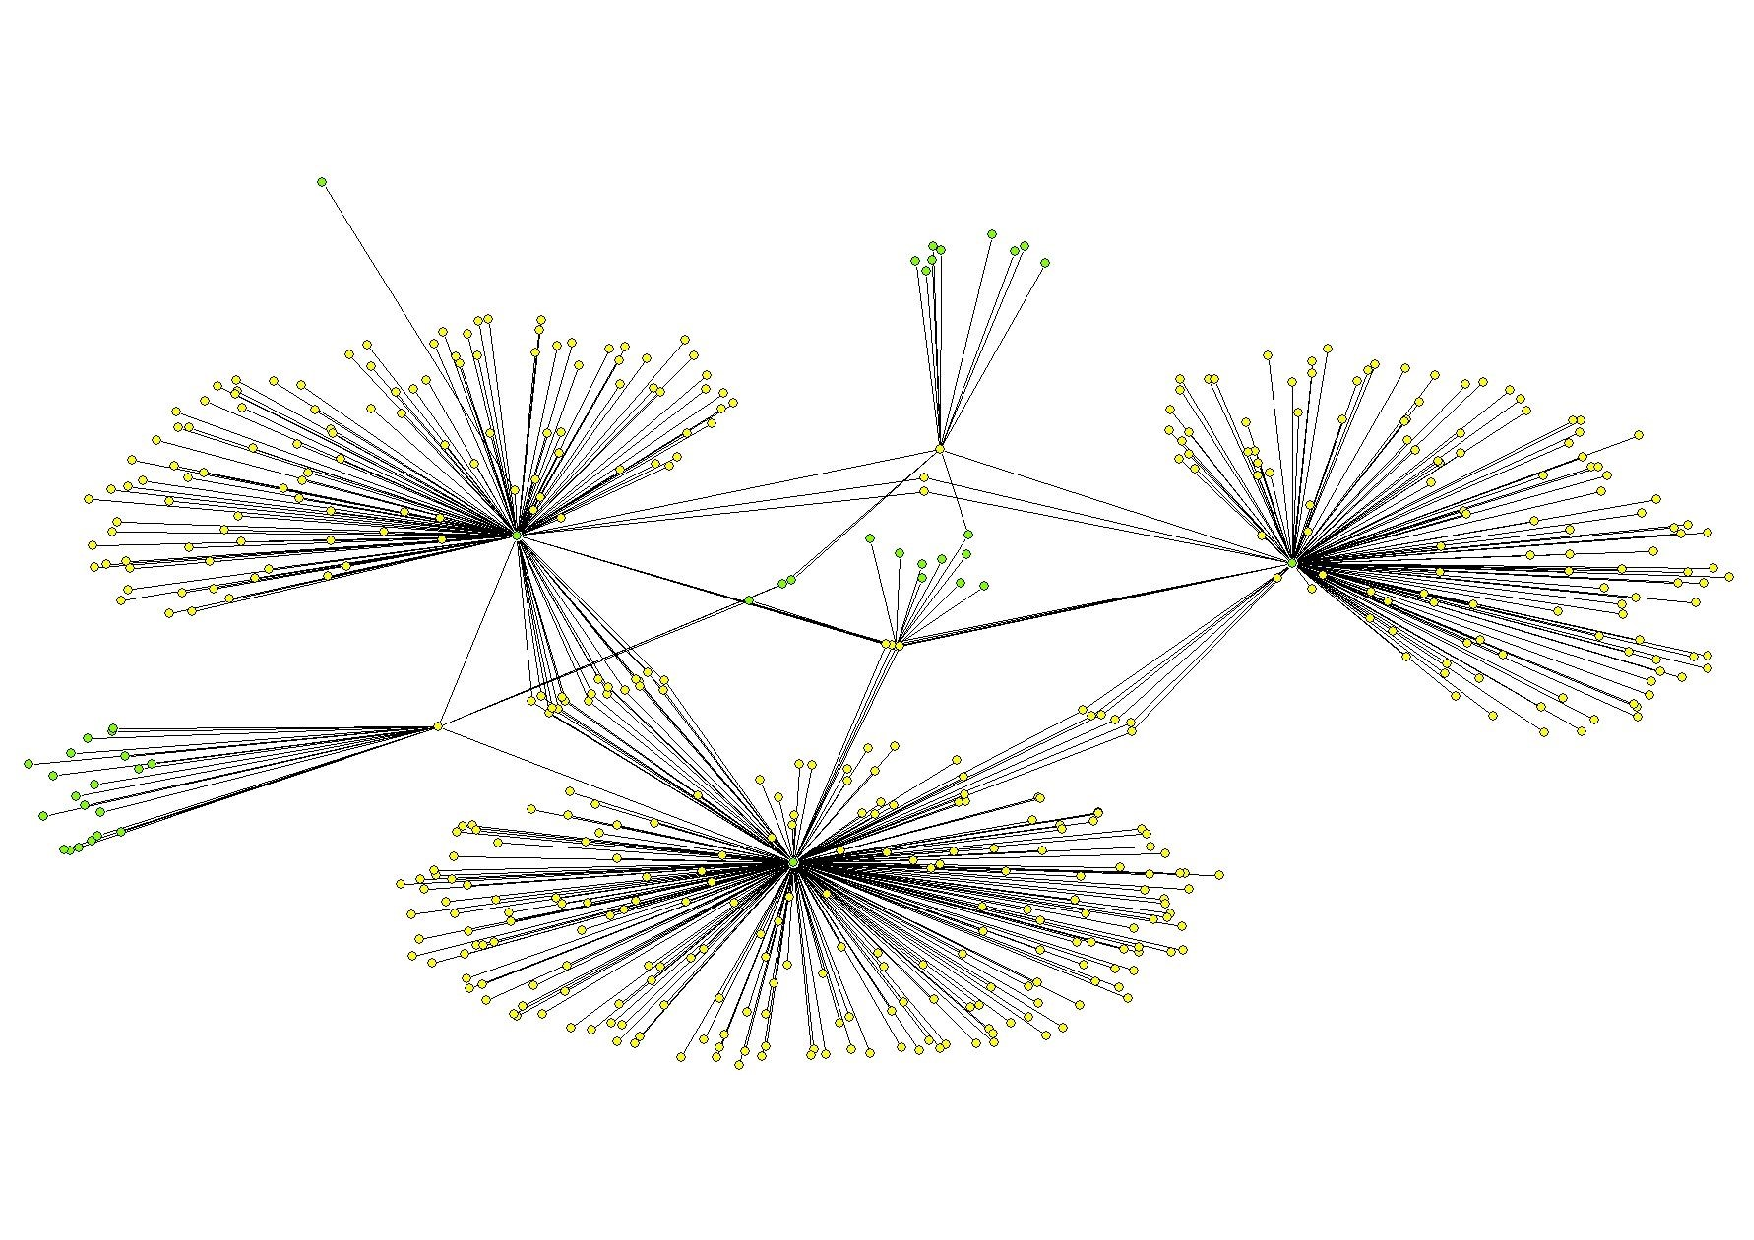
\includegraphics[scale=0.55]{rede_artistas_orquestras_PROVISORIO.pdf}

	%	\fonte{Elaboração do autor a partir de dados disponíveis online}

	%\end{figure}







	\postextual

	\citeoption{abnt-full-initials=yes}

	\bibliography{BIBDOUTORADO, abnt-options}

















	\chapter*[Anexo 1]{Anexo 1 - Trabalhos consultados}

	\addcontentsline{toc}{chapter}{Anexo 1 - Trabalhos consultados}





	\begin{SingleSpace}

	\begin{footnotesize}

	\begin{center}



	\begin{longtable}{p{4cm}lp{4cm}p{4cm}}







		\hline

		\textbf{Autores} &\textbf{Ano} & \textbf{Journal} & \textbf{Assunto}\\

		\hline

		\hline

		\endfirsthead

		\hline

		\endhead

		\hline

		\endfoot

		\hline

		\hline

		\endlastfoot



		Roy, Tirthankar & 1998 & Contributions to Indian Sociology & Indian classical music\\

		Waterman, Stanley & 2010 & Contemporary Jewry & Israel culture/music\\

		Coaldrake, Kimi	& 2012 & Japanese Studies & Japanese popular music\\

		Menger, Pierre-Michel & 1991 & Cahiers de recherche sociologique & Factors affecting market structure and music evaluation\\

		Menger, Pierre-Michel & 1983 & Sociologie du Travail & Division of musical labor\\

		Buchholz, Larissa & 2013 & NA & Global rules of art\\

		Etzioni, Amitai & 1998 & Journal of Socio-Economics & Taste for classical music\\

		Roebuck, James C & 2000 & American Sociological Association & Gendered-habitus, and the sexual division of labor\\

		Francois, Pierre & 2004 & Sociologie du Travail & Ilness of cost / concert market / musicians labor market\\

		Gligorijevic, Jelena & 2014 & International Journal of Cultural Policy & Music festival / Serbia\\

		Hofman, Ana & 2014 & Dve domovini / Two Homelands & Identification and affiliation / trumpet orchestra music / Balkan music\\

		Segnini, Liliana Rolfsen Petrilli & 2011 & Estudos de Sociologia & Music job market\\

		Epstein, Louis K & 2013 & NA & Music patronage\\

		Kaleta, Andrzej & 2004 & Polish Sociological Review & Cultural Activity of Rural Inhabitants\\

		Zolberg, Vera & 1996 & International Sociology & Music patronage\\

		Mauskapf, Michael G & 2012 & NA & Music patronage / economic and cultural sustainability\\

		Borowiecki, Karol J; O'Hagan, John W & 2012 & Historical Social Research/Historische Sozialforschung & Historical Patterns / The case of classical composers\\

		Fisher, Timothy C G; Preece, Stephen B & 2003 & Poetics & Culture of comsumption\\

		Dowd, Timothy J; Liddle, Kathleen; Lupo, Kim; Borden, Anne. & 2002 & Poetics & Musical Canon\\

		Kremp, Pierre-Antoine & 2010 & Social Forces & Musical Canon\\

		Broughton, Andrea & 2001 & European Journal of Industrial Relations & Collective Bargaining in the Arts and Culture Sector\\

		Hughes, Patricia; Luksetich, William; Rooney, Patrick & 2014 & Nonprofit Management \& Leadership & Music patronage\\

		Glynn, Mary Ann & 2002 & Poetics & Organizational Crisis / Institutional Shifts / Musical Canon\\

		Wood, Roy D & 2010 & NA & Conductor leadership style, musician employment status, organizational participation to orchestra musician job satisfaction\\

		Bijsterveld, Karin; Schulp, Marten & 2004 & Social Studies of Science & Innovation in classical music instruments\\

		Luthje, Corinna & 2010 & Medien \& Kommunikationswissenschaft & Classical Music in German Commercial Radio Programming\\

		McCormick, Lisa & 2009 & Cultural Sociology & International Music Competition\\

		Lee, Steve Sungchu & 2007 & NA & Musical stratification / aesthetics\\

		Francois, Pierre & 2006 & Revue francaise de Sociologie & Early Music Market\\

		Santoro, Marco & 2013 & European Societies & Institutions / music market\\

		Abreu, Paula & 2009 & Revista Critica de Ciencias Sociais & Portuguese phonographic industry\\

		Watson, Allan & 2012 & Global Networks & Urban networks of music production / Itunes\\

		Nicolau, Michel & 2010 & International Sociological Association & National Identity / Brazilian music\\

		Janowska, Anna Anetta & 2011 & Societes & Digital Revolution / Reconrding Industry\\

		Abreu, Paula & 2004 & Revista Critica de Ciencias Sociais & Territorial dynamics of cultural markets / Portuguese music\\

		Shin, Eui Hang; Oh, Joong-Hwan & 2002 & East Asia: An International Quarterly & Relationships between two different sets of actors - songwriters \& singers / Korean popular music industry\\

		Salganik, Matthew J; Watts, Duncan J & 2008 & Social Psychology Quarterly & Self-fulfilling Prophecies in an Artificial Cultural Market\\

		Dowd, Timothy J & 2003 & Comparative Social Research & Structural Power and the Construction of Markets / R\&B\\

		DeNora, Tia & 2013 & European Societies & Markets and socio-cultural practices\\

		Menger, Pierre-Michel & 2002 & Annales & Genius / Beethoven\\

		Pethig, Rudiger; Cheng, Sao-Wen & 2002 & Schmollers Jahrbuch & Cultural Capital / Consumption of Cultural Services\\

		Salganik, Matthew J & 2007 & NA & Success and failure in cultural markets\\

		Kasaras, Kostas; Klimis, George Michael; Michailidou, Martha & 2012 & Contemporary Social Science: Journal of the Academy of Social Sciences & Musical tastes / experimental study\\

		Ginsburgh, Victor & 2003 & Journal of Economic Perspectives & Expertise in the arts influence success\\



	\end{longtable}

\end{center}

\end{footnotesize}

\end{SingleSpace}






	\chapter*[Anexo 2]{Anexo 2 - Questionário online}

	\addcontentsline{toc}{chapter}{Anexo 2 - Questionário online}



	[\textbf{Primeira página - Concordância}]
	
	QUESTIONÁRIO SOCIOMÉTRICO DIRECIONADO A MÚSICOS E PROFESSORES
	
	Olá. A pesquisa de tese em andamento intitulada ``A Construção Social da Qualidade num Mercado de Música de Concerto'' de autoria de Neylson Crepalde visa investigar a construção de um padrão de qualidade amplamente aceito por orquestras, músicos e público com o qual todos assumem compromisso e sobre o qual todos agem na construção do mercado da música de concerto. O estudo está sendo realizado de uma perspectiva relacional. Desse modo, uma parte das perguntas a serem feitas aos entrevistados são o que a literatura chama de “geradores de nomes”, ou seja, perguntas que demonstram algum tipo de relação entre dois indivíduos ou organizações.
	
	Um dos principais objetivos do estudo é reconstruir a estrutura de relações entre músicos e entre organizações para, a partir dela, entender como emerge o conceito de qualidade.
	
	A tese está sendo orientada pelo professor Silvio Salej Higgins (UFMG/Brasil) e tem coorientação do prof. Emmanuel Lazega (CSO – SciencesPo/França).
	
	Muito embora esta pesquisa de tese não tenha passado por nenhum comitê de ética em pesquisa, todos os procedimentos éticos recomendados estão sendo adotados. Nenhum nome, seja de organização ou indivíduo será divulgado (a menos que haja expresso desejo da organização ou indivíduo) e a participação é voluntária. Os participantes possuem o direito de retirar sua participação a qualquer momento da pesquisa. É importante, entretanto, salientar o quão importante é a participação de cada convidado para o sucesso da pesquisa de tese.
	
	Para quaisquer dúvidas ou esclarecimentos, os contatos dos responsáveis pela pesquisa estão disponibilizados abaixo:
	
	Neylson Crepalde – Doutorando
	Telefone: +55 31 98554 0770
	E-mail: neylsoncrepalde@gmail.com
	
	Silvio Salej Higgins – Orientador
	E-mail: sisahi@yahoo.com.br
	
	\vspace{1cm}
	
	[\textbf{Segunda Página - Informações gerais}] % UNDER CONSTRUCTION......
	
	\begin{enumerate}
		\item Qual é o seu nome: 
		
		\item Sexo?
		\begin{itemize}
			\item Masculino
			\item Feminino
			\item Outro
		\end{itemize}
		
		\item Qual é a sua escolaridade?
		\begin{itemize}
			\item Ensino médio - incompleto
			\item Ensino médio - completo
			\item Superior - incompleto
			\item Superior - completo
			\item Mestrado - incompleto
			\item Mestrado - completo
			\item Doutorado - incompleto
			\item Doutorado - completo
		\end{itemize}
		
		\item Quanto à cor da pele, o(a) senhor(a) se considera...?
		\begin{itemize}
			\item Branco
			\item Preto
			\item Pardo
			\item Amarelo
			\item Indígena
			\item Outro
		\end{itemize}
		
		\item Qual é a sua idade?
		

		\item Qual é o seus estado civil?
		\begin{itemize}
			\item Casado
			\item Solteiro
			\item Divorciado
			\item Viúvo
			\item Outro
		\end{itemize}
		
		
		\item O(a) senhor(a) tem filhos? Quantos?
		
		
		[\textbf{Terceira página - Atividades musicais}]  
		
		
		\item Qual é a sua principal atividade como músico?
		\begin{itemize}
			\item Intrumentista
			\item Cantor
			\item Maestro
			\item Professor
			\item Outro
		\end{itemize}
		
		

		
		\item O(a) senhor(a) toca em alguma orquestra? Qual ou quais?
		
		\item O(a) senhor(a) ensina em alguma escola de música, faculdade/universidade? Qual?
		\item Se sim, quantos alunos possui hoje?
		\item Qual foi a sua renda total no último mês considerando todas as orquestras nas quais o(a) senhor(a) tocou?
		\item Qual foi a sua renda total no último mês considerando seu trabalho com as orquestras e todas as outras atividades que o(a) senhor(a) exerce?
		
		\item Com que frequência o(a) senhor(a) assiste a concertos?
		\begin{itemize}
			\item Uma ou duas vezes por ano
			\item Uma ou duas vezes a cada três meses
			\item Uma ou duas vezes por mês
			\item Uma vez por semana
			\item Mais de uma vez por semana
		\end{itemize}
		
		
		
		[\textbf{Quarta página - Bloco relacional}]
		
		
		\item Se o(a) senhor(a) precisasse de aconselhamento sobre a interpretação de alguma peça, independente do período ou do estilo da obra, a quem o(a) senhor(a) pediria conselho? Mencione quantas pessoas o(a) senhor(a) quiser.
		
		\item O(a) senhor(a) costuma se encontrar com outros músicos em ocasiões sociais fora do horário de trabalho? Com quem o(a) senhor(a) se encontra? Mencione quantas pessoas o(a) senhor(a) quiser.
		
		\item Se o(a) senhor(a) fosse indicar um músico para uma excelente posição em uma orquestra, a quem o(a) senhor(a) indicaria? Mencione quantas pessoas o(a) senhor(a) quiser independente do instrumento.
		
		\item Se o(a) senhor(a) fosse responsável por organizar um recital ou um concerto no qual o(a) senhor(a) fosse tocar, independente da instrumentação das obras que o senhor poderia escolher, a quem o(a) senhor(a) convidaria para tocar com o(a) senhor(a)? Mencione quantas pessoas o(a) senhor(a) quiser.
		
		\item Para o(a) senhor(a), quais são as orquestras em Belo Horizonte que possuem a melhor qualidade? Por favor, cite da que possui a melhor qualidade para a que possui a pior dentre elas.
		
		\item Porque a orquestra que o(a) senhor(a) disse ser a melhor é a melhor? Cite quantas razões o(a) senhor(a) quiser.
		
		\item Caso o(a) senhor(a) seja também professor(a), como o(a) senhor(a) faz seus alunos entenderem o que é necessário para uma boa performance?
		
		
		
		
		[\textbf{Quinta página - Bloco Contextual}]
		
		
		\item Em qual país o(a) senhor(a) nasceu?
		\item Em qual cidade o(a) senhor(a) nasceu?
		\item Por quantos ANOS o(a) senhor(a) estuda música?
		\item Por quantos ANOS o(a) senhor(a) tem trabalhado como músico/musicista profissional?
		\item Em qual instituição o(a) senhor(a) recebeu a maior parte de sua educação musical?
		\item E em segundo lugar?
		\item Com qual professor o(a) senhor(a) estudou pelo período mais longo?
		\item E em segundo lugar?
		
	\end{enumerate}
	
	Muito obrigado pela sua participação. Sua colaboração é imprescindível para o sucesso dessa pesquisa. Novamente, muito obrigado!
	
	
	\newpage
	
	
	
	\chapter*[Questionário - organizações]{Anexo 3 -- Questionário sociométrico - organizações}
	
	%Good day. I want to thank you very much for your participation and assure that it is extremely important for the success of this PhD research.
	
	Bom dia. Quero agradecer muitíssimo pela sua participação e assegurar o quanto ela é importante para o sucesso desta pesquisa de Doutorado.
	
	\vspace{1cm}
	\begin{enumerate}
		%\item Let's start with your professional partnerships. Could you name all the professionals that you relate with regularly? By professionals I mean every company with whom you have relations, economic or other, for example, advisement, collaboration, resources exchange, etc.
		
		\item Vamos começar com suas parcerias profissionais. O senhor poderia nomear todos os empresas com as quais a organização se relaciona regularmente? Me refiro aqui a qualquer companhia com a qual a orquestra tenha relações, econômicas ou de outra natureza, como por exemplo, aconselhamento, colaboração, troca de recursos, etc.
		
		%\item What is the main activity of each of these professionals?
		
		\item Vamos retomar cada uma dessas empresas. Qual é a principal atividade de cada uma delas?
		
		%\item I would like to retake each of this professionals that you mentioned. What is the relation that you would say you have with each one of them?
		
		\item Vamos retomar mais uma vez a lista de empresas que o senhor mencionou. Qual é a relação que o senhor diria que a orquestra possui com cada um?
		\begin{itemize}
			\item Uma relação de fornecedor e cliente, apenas.
			\item Uma parceria
			\item Uma colaboração
			\item Uma relação de aconselhamento
			\item Outra
		\end{itemize}
		
		%\item What is the organization's structure? Is there an organizational chart that I could consult?
		\item Qual é a estrutura da organização? Existe um organograma que eu possa consultar?
		
		%\item What is the organization's budget?     
		
		\item Qual é o orçamento total da organização?
		
		%\item You did mention the State as one of your partners (What about the State?) How many contracts do you have with the State? What is it's share in your budget?
		
		\item O senhor mencionou o Estado como um de seus parceiros (E o Estado?) Quantos contratos a orquestra possui com o Estado? Qual é a sua parcela de contribuição no orçamento?
		
		%\item What would you say is your organization's style within the market?
		

		%\item In what spaces does the orchestra usually play? How many seats available?
		
		\item Em quais espaços a orquestra normalmente toca? Quantos assentos tem disponíveis em cada um?
		
		%\item What is the ticket price for each of the concert series? Is there variation on ticket price according to the place in the concert room? How many tickets are made available with each price?
		\item Qual é o preço do ingresso para cada série de concertos? Há uma variação no preço de acordo com o lugar na sala? Quantos ingressos são disponibilizados por cada faixa de preço?
		
		%\item How much does the organization spend with musicians paycheck?
		\item Quanto a orquestra gasta com a folha de pagamento dos músicos?
		
		%\item Besides musicians and guests paycheck, what would you say are other artistic expenses of a performance?
		\item Além da folha de pagamento dos músicos e convidados, o senhor diria que há outras despesas artísticas relacionadas às performances?
		
		%\item Does the orchestra have some incentive for the musicians to feel motivated, pleased and satisfied with their jobs? Could you list them, please?
		\item A orquestra oferece incentivos aos músicos para que eles se sintam motivados, felizes e satisfeitos com seu emprego? O senhor poderia listá-los, por favor?
		
	\end{enumerate}
	
	Muito obrigado pela participação!



\end{document}